% chapters/ch05.tex - 第 5 章: 流形上的伪微分算子

\chapter[流形上的伪微分算子]{流形上的\\伪微分算子}\label{ch:05}

我们现在展示如何借助局部坐标卡将 $\R^n$ 上的伪微分算子代数转移至任意光滑流形上. 关键输入是 $m$ 阶伪微分算子类在 $\R^n$ 坐标变换下的不变性 (第~\ref{sec:5.1}~节). 我们在第~\ref{sec:5.2}--\ref{sec:5.3}~节中回顾流形, 向量丛, 密度以及流形上的微分算子. 随后在第~\ref{sec:5.4}--\ref{sec:5.8}~节中正式定义流形上的伪微分算子并深入探讨其算子代数与符号性质; 我们相当详细地解释这一向流形的过渡.

在流形上定义伪微分算子时, 通常存在两种处理途径. 第一种途径是强制要求所有伪微分算子都是\textbf{适正支集的} (properly supported, 定义~\ref{def:5.30}), 在此情形下任意两个伪微分算子均可自由复合; 其缺点在于, 即使在 $\R^n$ 上, 像 $\langle D \rangle^s$ ($s \notin 2\N_0$) 这样简单的伪微分算子也不符合条件. 第二种途径是对 Schwartz 核的支集不施加任何人为限制 (定义~\ref{def:5.21}); 其缺点是两个这样的伪微分算子的复合一般而言没有定义 (但参见定理~\ref{thm:5.32}). 与欧氏空间 $\R^n$ 不同, 一般流形 $M$ 并不天然具备一个全局度量来测量 Schwartz 核在对角线外的快速衰减 (对比推论~\ref{cor:4.9}), 因而并不存在自然的第三种折中选择. 为了保持理论的最大一般性, 本书在此采用第二种途径. (在紧流形上, 两种途径当然完全等价.)

作为伪微分演算的第一个应用, 我们可以对紧流形上的椭圆算子及其 Fredholm 性质给出简洁的处理: 首先在光滑函数范畴下展开 (第~\ref{sec:5.9}~节), 接着在流形上建立 Sobolev 空间之后 (第~\ref{sec:5.10}~节), 在 Sobolev 空间范畴下讨论 (第~\ref{sec:5.11}--\ref{sec:5.12}~节). 作为一个简单的非线性应用, 我们讨论单值化定理的一个局部版本 (第~\ref{sec:5.13}~节). 作为分析非椭圆算子的一点准备, 我们重新讨论换位子的主符号以及它与 $T^* M$ 的辛结构的关系 (第~\ref{sec:5.14}~节). 最后, 我们描述如何把迄今建立的理论适配到半经典设定 (第~\ref{sec:5.15}~节).

\section{局部坐标不变性}\label{sec:5.1}
\index{zuobiaobianhuan@坐标变换 (change of variables)}%
\index{Kuranishi jiqiao@Kuranishi 技巧 (Kuranishi trick)}%

我们证明命题~\ref{prop:3.3} 最后一部分在伪微分算子情形下的类比.

\begin{definition}[具有受限 Schwartz 核的伪微分算子]\label{def:5.1}
设 $\Omega \subset \R^n$ 为开集. 则
\begin{equation}\label{eq:5.1}
    \Psi_{\mathrm{c}}^m(\Omega) \defeq \left\{ A \in \Psi^m(\R^n) : \supp K_A \text{ 是 } \Omega \times \Omega \text{ 的紧子集} \right\},
\end{equation}
其中 $K_A \in \TempDistr(\R^{2n})$ 表示算子 $A$ 的 Schwartz 核.
\end{definition}

\begin{theorem}[坐标变换下的伪微分算子]\label{thm:5.2}
设 $\Omega, \Omega' \subset \R^n$ 为开集, 且 $\kappa \colon \Omega \to \Omega'$ 为微分同胚. 给定 $A \in \Psi_{\mathrm{c}}^m(\Omega')$, 对 $u \in \SmoothComp(\R^n)$ 定义拉回算子
\[
    A_\kappa u \defeq \kappa^* A\left( (\kappa^{-1})^* (u|_\Omega) \right).
\]
则 $A_\kappa \in \Psi_{\mathrm{c}}^m(\Omega)$, 且映射 $\Psi_{\mathrm{c}}^m(\Omega') \ni A \mapsto A_\kappa \in \Psi_{\mathrm{c}}^m(\Omega)$ 是双射. 此外,
\begin{equation}\label{eq:5.2}
    \sigma_m(A_\kappa)(x, \xi) = \sigma_m(A)\left( \kappa(x), (\kappa'(x)^T)^{-1} \xi \right).
\end{equation}
(见图~\ref{fig:5.1}.)
\end{theorem}

\begin{figure}[htbp]
    \centering
    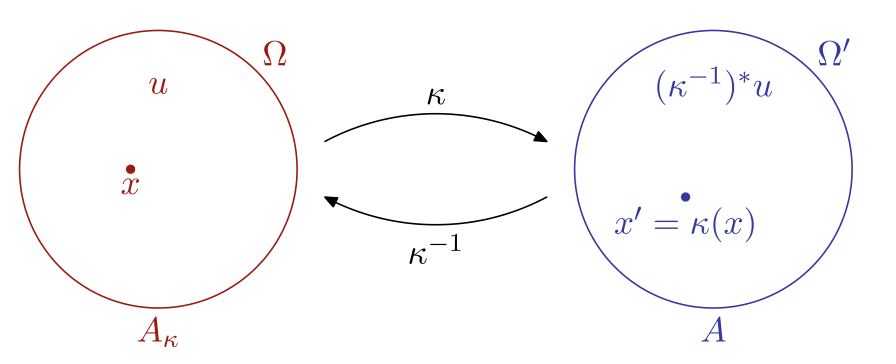
\includegraphics[width=0.72\textwidth]{figs/fig5_1_clean.png}
    \caption{伪微分算子在局部微分同胚坐标变换下的拉回几何示意.}
    \label{fig:5.1}
\end{figure}

\begin{proof}[定理~\ref{thm:5.2} 的证明]
将 $A$ 写为左量化 $A = \Op_L(a)$, 其中 $a \in S^m(\R^n; \R^n)$. 选取 $\psi \in \SmoothComp(\Omega')$ 使得在 $\supp K_A$ 上 $\psi(x) \psi(y) = 1$; 从而 $K_A(x, y) = \psi(x) K_A(x, y) \psi(y)$, 因此
\begin{equation}\label{eq:5.3}
    A = \Op\left( \psi(x) a(x, \xi) \psi(y) \right).
\end{equation}
我们在对角线附近进行局部化: 对待定的充分小常数 $\epsilon > 0$, 选取 $\chi_\epsilon(x, y) \in \Smooth(\R^{2n})$ 满足: 当 $|x - y| < \epsilon$ 时 $\chi_\epsilon(x, y) = 1$, 而当 $|x - y| > 2\epsilon$ 时 $\chi_\epsilon(x, y) = 0$. 则
\begin{equation}\label{eq:5.4}
    K_{A_\epsilon} \defeq \Op(a_\epsilon), \qquad a_\epsilon(x, y, \xi) \defeq \chi_\epsilon(x, y) \psi(x) \psi(y) a(x, \xi),
\end{equation}
是某个算子 $A_\epsilon \in \Psi_{\mathrm{c}}^m(\Omega')$ 的 Schwartz 核. 差算子
\begin{equation}\label{eq:5.5}
    R_\epsilon \defeq A - A_\epsilon
\end{equation}
是 Schwartz 核支集完全位于对角线外部的伪微分算子, 从而 $R_\epsilon \in \Psi^{-\infty}(\R^n)$, 并且其 Schwartz 核满足 $K_{R_\epsilon} \in \SmoothComp(\Omega' \times \Omega')$. 我们随后有
\begin{equation}\label{eq:5.6}
    \begin{aligned}
        (R_\epsilon)_\kappa u(x) &= \int_{\Omega'} K_{R_\epsilon}(\kappa(x), y') u(\kappa^{-1}(y')) \,\dd y' \\
        &= \int_\Omega K_{R_\epsilon}(\kappa(x), \kappa(y)) |\!\det \kappa'(y)| u(y) \,\dd y.
    \end{aligned}
\end{equation}
因此, $(R_\epsilon)_\kappa$ 的 Schwartz 核在 $x, y \in \Omega$ 时等于 $K_{R_\epsilon}(\kappa(x), \kappa(y)) |\!\det \kappa'(y)|$, 在其余位置为 0. 从而 $(R_\epsilon)_\kappa \in \Psi_{\mathrm{c}}^{-\infty}(\Omega)$.

现在只需证明 $(A_\epsilon)_\kappa \in \Psi_{\mathrm{c}}^m(\Omega)$. 首先假定 $a \in S^{-\infty}(\R^n; \R^n)$. 则
\begin{equation}\label{eq:5.7}
    \begin{aligned}
        (A_\epsilon)_\kappa u(x) &= (2\pi)^{-n} \iint_{\R^n \times \Omega'} \ee^{\ii (\kappa(x) - y') \cdot \xi'} a_\epsilon(\kappa(x), y', \xi') u(\kappa^{-1}(y')) \,\dd y' \,\dd\xi' \\
        &= (2\pi)^{-n} \iint_{\R^n \times \Omega} \ee^{\ii (\kappa(x) - \kappa(y)) \cdot \xi'} a_\epsilon(\kappa(x), \kappa(y), \xi') |\!\det \kappa'(y)| u(y) \,\dd y \,\dd\xi',
    \end{aligned}
\end{equation}
因此 $(A_\epsilon)_\kappa$ 的 Schwartz 核为
\begin{equation}\label{eq:5.8}
    \begin{aligned}
        K_{(A_\epsilon)_\kappa}(x, y) &= (2\pi)^{-n} \int_{\R^n} \ee^{\ii (\kappa(x) - \kappa(y)) \cdot \xi'} b_\epsilon(x, y, \xi') \,\dd\xi', \\
        b_\epsilon(x, y, \xi') &\defeq a_\epsilon(\kappa(x), \kappa(y), \xi') |\!\det \kappa'(y)| \\
        &= \chi_\epsilon(\kappa(x), \kappa(y)) \psi(\kappa(x)) \psi(\kappa(y)) a(\kappa(x), \xi') |\!\det \kappa'(y)|.
    \end{aligned}
\end{equation}
为了将 $K_{(A_\epsilon)_\kappa}$ 识别为伪微分算子的 Schwartz 核, 我们使用著名的 \textbf{Kuranishi 技巧} (Kuranishi trick). 将指数进行 Taylor 积分展开: 记 $\kappa_j$ 为 $\kappa$ 的第 $j$ 个分量, 我们有
\begin{equation}\label{eq:5.9}
    \kappa_j(x) - \kappa_j(y) = \sum_{k=1}^n \Phi_{jk}(x, y) (x_k - y_k), \qquad \Phi_{jk}(x, y) \defeq \int_0^1 \partial_{x_k} \kappa_j(y + t(x - y)) \,\dd t,
\end{equation}
从而有内积恒等式:
\begin{equation}\label{eq:5.10}
    (\kappa(x) - \kappa(y)) \cdot \xi' = \langle \Phi(x, y) (x - y), \xi' \rangle = \langle x - y, \Phi(x, y)^T \xi' \rangle,
\end{equation}
其中 $\Phi(x, y) = (\Phi_{jk}(x, y))_{j, k=1, \ldots, n}$, 且 $\langle \cdot, \cdot \rangle$ 为 $\R^n$ 上的标准内积. 注意到在对角线上
\begin{equation}\label{eq:5.11}
    \Phi(x, x) = \kappa'(x)
\end{equation}
处处可逆 (因为 $\kappa$ 为微分同胚). 在紧支撑集
\begin{equation}\label{eq:5.12}
    (x, y) \in \supp\left( \chi_\epsilon(\kappa(x), \kappa(y)) \psi(\kappa(x)) \psi(\kappa(y)) \right) \subset \kappa^{-1}(\supp\psi) \times \kappa^{-1}(\supp\psi) \subset \Omega \times \Omega
\end{equation}
上, 当 $\epsilon > 0$ 充分小时满足 $|\kappa(x) - \kappa(y)| \le 2\epsilon$, 从而矩阵 $\Phi(x, y)$ 在该区域内处处一致可逆. 在式~\eqref{eq:5.8} 中做线性变量代换 $\xi = \Phi(x, y)^T \xi'$, 即 $\xi' = (\Phi(x, y)^T)^{-1} \xi$, 得到
\begin{equation}\label{eq:5.13}
    \begin{aligned}
        (A_\epsilon)_\kappa &= \Op(c_\epsilon), \\
        c_\epsilon(x, y, \xi) &\defeq b_\epsilon\left( x, y, (\Phi(x, y)^T)^{-1} \xi \right) |\!\det \Phi(x, y)|^{-1} \\
        &= a_\epsilon\left( \kappa(x), \kappa(y), (\Phi(x, y)^T)^{-1} \xi \right) |\!\det \Phi(x, y)|^{-1} |\!\det \kappa'(y)|.
    \end{aligned}
\end{equation}
我们断言 $c_\epsilon \in S^{-\infty}(\R^n \times \R^n; \R^n)$; 更一般地, 若 $a \in S^m(\R^n; \R^n)$, 则由式~\eqref{eq:5.13} 定义的符号 $c_\epsilon$ 属于 $S^m(\R^n \times \R^n; \R^n)$ 且连续依赖于 $a$. 忽略平滑的 Jacobi 行列式因子, 直接微分计算可知:
\begin{equation}\label{eq:5.14}
    \begin{aligned}
        &\partial_x^\alpha \partial_y^\beta \partial_\xi^\gamma \left( a_\epsilon\left( \kappa(x), \kappa(y), (\Phi(x, y)^T)^{-1} \xi \right) \right) \\
        &= \sum_{\substack{|\alpha'| + |\alpha''| \le |\alpha| \\ |\beta'| + |\beta''| \le |\beta|}} F_{\alpha \alpha' \alpha'' \gamma}^{\beta \beta' \beta''}(x, y) \xi^{\alpha'' + \beta''} (\partial_x^{\alpha'} \partial_y^{\beta'} \partial_\xi^{\gamma + \alpha'' + \beta''} a_\epsilon)\left( \kappa(x), \kappa(y), (\Phi(x, y)^T)^{-1} \xi \right),
    \end{aligned}
\end{equation}
其中 $F_{\alpha \alpha' \alpha'' \gamma}^{\beta \beta' \beta''} \in \SmoothComp(\Omega \times \Omega)$ 仅依赖于 $\kappa$. 由于 $\Phi(x, y)^T$ 及其逆在 $\supp a_\epsilon$ 上一致有界, 存在常数 $c, C > 0$ 使得在 $\supp a_\epsilon$ 上有 $c |\xi| \le |(\Phi(x, y)^T)^{-1} \xi| \le C |\xi|$. 因此式~\eqref{eq:5.14} 被 $\langle \xi \rangle^{m - |\gamma|}$ 乘以 $a$ 的一个连续半范数所界, 正合所需. 最后, 给定 $a \in S^m(\R^n; \R^n)$, 我们选取 $a^{(j)} \in S^{-\infty}(\R^n; \R^n)$ ($j \in \N$), 它们在 $S^m(\R^n; \R^n)$ 中一致有界, 且当 $j \to \infty$ 时在 $S^{m+1}(\R^n; \R^n)$ 中收敛到 $a$. 于是相应的符号 $c_\epsilon^{(j)}$ 在 $S^m(\R^n \times \R^n; \R^n)$ 中一致有界, 并在 $S^{m+1}(\R^n \times \R^n; \R^n)$ 中收敛到 $c_\epsilon$. 令 $A_\epsilon^{(j)} = \Op(a_\epsilon^{(j)})$, 其中 $a_\epsilon^{(j)}$ 按式~\eqref{eq:5.4} 由 $a^{(j)}$ 定义, 则对所有 $u \in \SmoothComp(\R^n)$ 有 $(A_\epsilon)_\kappa u = \lim_{j \to \infty} (A_\epsilon^{(j)})_\kappa u$; 又由式~\eqref{eq:4.24}, 当 $j \to \infty$ 时 $(A_\epsilon^{(j)})_\kappa u = \Op(c_\epsilon^{(j)}) u \to \Op(c_\epsilon) u$, 从而我们在一般情形下确立了式~\eqref{eq:5.13}.

关于主符号, 我们有 $\sigma_m(A_\kappa) = \sigma_m((A_\epsilon)_\kappa) = \sigma_m(\Op(c_\epsilon))$, 它可以从约化公式~\eqref{eq:4.50} 的 (首项) 读出: 利用式~\eqref{eq:5.11}, 它由 $S^m(\R^n; \R^n) / S^{m-1}(\R^n; \R^n)$ 中的下述等价类给出:
\[
    c_\epsilon(x, x, \xi) = b_\epsilon\left( x, x, (\kappa'(x)^T)^{-1} \xi \right) |\!\det \kappa'(x)|^{-1} = a_\epsilon\left( \kappa(x), \kappa(x), (\kappa'(x)^T)^{-1} \xi \right) = a\left( \kappa(x), (\kappa'(x)^T)^{-1} \xi \right).
\]
证明完成.
\end{proof}

\section{流形, 光滑函数, 丛与密度}\label{sec:5.2}
\index{guanghua liuxing@光滑流形 (smooth manifolds)}%
\index{xiangliangcong@向量丛 (vector bundles)}%
\index{miducong@密度丛 (density bundles)}%

我们回顾:

\begin{definition}[光滑流形]\label{def:5.3}
设 $n \in \N$. 一个 $n$ 维\textbf{光滑流形} (smooth manifold) 是一个第二可数的 Hausdorff 拓扑空间 $M$, 满足:
\begin{enumerate}
    \item 对每个点 $p \in M$, 存在开邻域 $U_p \ni p$ 以及同胚映射 $F_p \colon U_p \to B(0, 1) = \{x \in \R^n : |x| < 1\} \subset \R^n$.
    \item 对所有满足 $U_p \cap U_q \neq \emptyset$ 的 $p, q \in M$, 转移映射
    \begin{equation}\label{eq:5.15}
        F_p \circ F_q^{-1}|_{F_q(U_p \cap U_q)} \colon F_q(U_p \cap U_q) \to F_p(U_p \cap U_q)
    \end{equation}
    是 $\R^n$ 开子集之间的光滑映射.
\end{enumerate}
\end{definition}

\begin{definition}[光滑结构与图册]\label{def:5.4}
设 $M$ 为光滑流形. $M$ 上的一个\textbf{图册} (atlas) 是坐标对集合 $\{(U_\alpha, F_\alpha)\}$ (其中 $M = \bigcup_\alpha U_\alpha$), 使得每个 $F_\alpha \colon U_\alpha \to F_\alpha(U_\alpha) \subset \R^n$ 均为微分同胚. 具有``任何其他图册都包含于其中''这一性质的图册称为\textbf{极大图册}, 或\textbf{光滑结构}. 极大图册中的每一个元素对 $(U, F)$ 称为一个 (局部坐标) \textbf{卡} (chart).
\end{definition}

在任意给定的光滑流形上, 始终存在唯一的极大图册. 我们还将遇到带边流形 (manifold with boundary) 以及更一般的带角柄流形 (manifold with corners): 它们的定义完全类似, 区别仅在于局部坐标卡映入 $\R^n$ 或 $[0, \infty) \times \R^{n-1}$ (对于带边流形), 以及 $[0, \infty)^k \times \R^{n-k}$ ($k \in \{0, \ldots, n\}$ 依赖于点 $p \in M$, 对应带角柄流形). 给定光滑流形 $M$, 其带角柄光滑子流形 $\Omega \subset M$ 是指满足对所有 $p \in \Omega$, 均存在局部坐标卡 $F \colon U \to F(U) \subset \R^n$ 使得
\begin{equation}\label{eq:5.16}
    \Omega \cap U = F^{-1}\left( [0, \infty)^k \times \R^{n-k} \right);
\end{equation}
带边光滑子流形正是仅允许 $k = 0, 1$ 的特例.

对 $k \in \N_0 \cup \{\infty\}$, 我们用 $\mathcal{C}^k(M)$ 表示所有满足在每个局部坐标卡下 $f \circ F_p^{-1} \in \mathcal{C}^k(B(0, 1))$ 的连续函数空间. 我们为 $\mathcal{C}^k(M)$ 配备标准的局部凸拓扑: 对于 $\Omega = B(0, 1) \subset \R^n$, $\mathcal{C}^k(\Omega)$ 通过紧集穷竭序列 $\Omega = \bigcup_{i=1}^\infty K_i$ ($K_1 \subset K_2 \subset \cdots, K_i \subset K_{i+1}^\circ$) 上的半范数族赋予 Fréchet 空间结构:
\begin{equation}\label{eq:5.17}
    |u|_{i, k} \defeq \max_{|\alpha| \le k} \max_{x \in K_i} |\partial^\alpha u(x)|.
\end{equation}
若改用半范数 $|\cdot|_{i, k}$ ($i \in \N$, $k \in \N_0$), 则 $\mathcal{C}^\infty(\Omega)$ 也成为 Fr\'echet 空间. 固定可数点集 $\{p_j\}$ 使得 $M = \bigcup_j U_{p_j}$, 我们随后用函数 $f \circ F_{p_j}^{-1} \in \mathcal{C}^k(B(0, 1))$ 的 $\mathcal{C}^k(B(0, 1))$-半范数来定义 $\mathcal{C}^k(M)$ 上的半范数.

对于紧支函数空间 $\mathcal{C}_{\mathrm{c}}^k(M)$, 首先对紧集 $K \subset M$ 定义 Fréchet 空间
\begin{equation}\label{eq:5.18}
    \dot{\mathcal{C}}^k(K) \defeq \left\{ u \in \mathcal{C}^k(M) : \supp u \subset K \right\}.
\end{equation}
现取 $M$ 的任一紧集穷竭 $M = \bigcup_{i=1}^\infty K_i$. 则 $\mathcal{C}_{\mathrm{c}}^k(M) = \bigcup_i \dot{\mathcal{C}}^k(K_i)$ 承载归纳极限拓扑, 参见 \cite[第~V.4~章]{RS72}. 它可以具体地定义如下. 取 $\phi_i \in \SmoothComp(K_{i+1}^\circ)$ 在 $K_i$ 附近等于 1, 并令 $\phi_0 \defeq 0$. 则 $\psi_i \defeq \phi_i - \phi_{i-1} \in \SmoothComp(K_{i+1}^\circ \setminus K_{i-1})$, 且在 $M$ 上 $\sum_i \psi_i = 1$. $\mathcal{C}_{\mathrm{c}}^k(M)$ 上的拓扑随后由半范数族
\begin{equation}\label{eq:5.19}
    |u|_{(w_i), (p_i)} \defeq \sup_{i} w_i p_i(\psi_i u)
\end{equation}
所生成, 其中 $(w_i)_{i \in \N}$ 为正实数列, $p_i$ 为 $\dot{\mathcal{C}}^k(K_{i+1} \setminus K_{i-1}^\circ)$ 上的连续半范数, $\sum_i \psi_i = 1$ 为从属单位分解 (详见习题~\ref{ex:5.1}--\ref{ex:5.3}).

向量丛的``实操''定义如下.

\begin{definition}[向量丛]\label{def:5.5}
设 $M$ 为 $n$ 维光滑流形. $M$ 上的实秩为 $k$ 的\textbf{实向量丛} (real vector bundle) 是一个三元组 $(\pi, E, M)$ (常记为 $\pi \colon E \to M$):
\begin{enumerate}
    \item $E$ 为 $(n+k)$ 维光滑流形, 且投影映射 $\pi \colon E \to M$ 光滑.
    \item 对任意 $p \in M$, 存在开邻域 $U_p \subset M$ 以及微分同胚 $\tau_p \colon \pi^{-1}(U_p) \to U_p \times \R^k$ 使得 $\pi(\tau_p^{-1}(q, v)) = q$.
    \item 对一切满足 $U_p \cap U_q \neq \emptyset$ 的 $p, q \in M$, 转移映射
    \begin{equation}\label{eq:5.20}
        \tau_{pq} \defeq \tau_p \circ \tau_q^{-1}|_{(U_p \cap U_q) \times \R^k} \colon (U_p \cap U_q) \times \R^k \to (U_p \cap U_q) \times \R^k
    \end{equation}
    具有形式 $\tau_{pq}(r, v) = (r, \Phi_{pq}(r) v)$, 其中 $\Phi_{pq} \colon U_p \cap U_q \to \mathrm{GL}(k)$ 是光滑映射.
\end{enumerate}
点 $p \in M$ 上的纤维记作 $E_p \defeq \pi^{-1}(p)$; 它具有实 $k$ 维向量空间的结构. $E$ 的零截面 $o$ 是 $E$ 的子流形, 在 $\pi^{-1}(U_p)$ 内局部地由 $\tau_p^{-1}(U_p \times \{0\})$ 给出. $E$ 的光滑截面是满足 $\pi \circ s = \operatorname{Id}_M$ 的光滑映射 $s \colon M \to E$; 光滑截面空间记作 $\mathcal{C}^\infty(M; E)$. 将 $\R^k$ 替换为 $\mathbb{C}^k$ 即得到\textbf{复向量丛}.

我们称映射 $\tau_p$ 为\emph{局部平凡化}. 若 $U_p$ 是坐标卡 $F \colon U_p \to F(U_p) \subset \R^n$ 的定义域, 则也称 $(F \times \operatorname{Id}) \circ \tau_p \colon \pi^{-1}(U_p) \to F(U_p) \times \R^k$ 为局部平凡化.
\end{definition}

\begin{definition}[纤维丛]\label{def:5.6}
设 $M$ 为 $n$ 维光滑流形; $F$ 为 $k$ 维光滑流形. 典型纤维为 $F$ 的\textbf{纤维丛} (fiber bundle) 是三元组 $(\pi, E, M)$, 具有如下性质:
\begin{enumerate}
    \item $E$ 为 $(n+k)$ 维光滑流形, 且投影映射 $\pi \colon E \to M$ 光滑.
    \item 对任意 $p \in M$, 存在开邻域 $U_p \subset M$ ($p \in U_p$) 以及微分同胚 $\tau_p \colon \pi^{-1}(U_p) \to U_p \times F$ 使得 $\pi(\tau_p^{-1}(q, f)) = q$.
    \item 对一切满足 $U_p \cap U_q \neq \emptyset$ 的 $p, q \in M$, 转移映射
    \begin{equation}\label{eq:5.21}
        \tau_{pq} \defeq \tau_p \circ \tau_q^{-1}|_{(U_p \cap U_q) \times F} \colon (U_p \cap U_q) \times F \to (U_p \cap U_q) \times F
    \end{equation}
    具有形式 $\tau_{pq}(r, f) = (r, \Phi_{pq}(r, f))$, 其中对每个 $r \in U_p \cap U_q$, $\Phi_{pq}(r, \cdot) \colon F \to F$ 是微分同胚.
\end{enumerate}
\end{definition}

回到向量丛. 注意: 为了唯一确定 (在同构意义下) 一个实秩 $k$ 向量丛, 只需具备如下数据与条件:
\begin{enumerate}
    \item $M$ 的一个由非空开子集组成的覆盖 $\{U_\alpha\}$.
    \item 对一切满足 $U_{\alpha\beta} \defeq U_\alpha \cap U_\beta \neq \emptyset$ 的 $\alpha, \beta$, 一个形如 $\tau_{\alpha\beta}(p, v) = (p, \Phi_{\alpha\beta}(p) v)$ 的映射 $\tau_{\alpha\beta} \colon U_{\alpha\beta} \times \R^k \to U_{\alpha\beta} \times \R^k$, 其中 $\Phi_{\alpha\beta} \colon U_{\alpha\beta} \to \mathrm{GL}(k)$ 光滑.
    \item 对一切 $p \in U_\alpha$, $v \in \R^k$ 有 $\tau_{\alpha\alpha}(p, v) = (p, v)$.
    \item 循环条件成立: 对满足 $U_{\alpha\beta\gamma} \defeq U_\alpha \cap U_\beta \cap U_\gamma \neq \emptyset$ 的 $\alpha, \beta, \gamma$, 在 $U_{\alpha\beta\gamma} \times \R^k$ 上有 $\tau_{\gamma\beta} \circ \tau_{\beta\alpha} = \tau_{\gamma\alpha}$.
\end{enumerate}
事实上, 此时可以令
\begin{equation}\label{eq:5.22}
    E \defeq \left( \bigsqcup_\alpha U_\alpha \times \R^k \right) / \sim
\end{equation}
唯一构筑向量丛, 其中等价关系 $\sim$ 定义为
\begin{equation}\label{eq:5.23}
    U_\alpha \times \R^k \ni (p, v) \sim (q, w) \in U_\beta \times \R^k \iff p = q, \ \tau_{\alpha\beta}(q, w) = (p, v).
\end{equation}
(循环条件保证该关系具有传递性, 而自反性由循环条件连同 $\tau_{\alpha\alpha} = \mathrm{Id}$ 推出.) 我们用 $[U_\alpha, (p, v)] \in E$ 表示等价类. 注意同一点 $p$ 可以落在两个 (或更多) 开集 $U_\alpha$ 与 $U_\beta$ 中, 但对 $v \in \R^k$ 通常有 $[U_\alpha, (p, v)] \neq [U_\beta, (p, v)]$. 投影映射 $\pi \colon E \to M$ 简单地由 $\pi([U_\alpha, (p, v)]) = p$ 给出. 作为局部平凡化, 我们可以取:
\begin{equation}\label{eq:5.24}
    \tau_\alpha \colon \{ [U_\alpha, (p, v)] : p \in U_\alpha \} \to U_\alpha \times \R^k, \qquad [U_\alpha, (p, v)] \mapsto (p, v).
\end{equation}

\begin{example}[切丛与余切丛]\label{eg:5.7}
取 $n$ 维流形 $M$ 由坐标卡 $F_i \colon U_i \to \R^n$ 构成的覆盖, 考虑 $\tau_{ij}(p, v) = (p, (F_i \circ F_j^{-1})'|_{F_j(p)} v)$. 所得的向量丛是 $M$ 的\textbf{切丛}, 记作 $TM$. 注意一个坐标卡 $F \colon U \to \R^n$ 通过 $U \times \R^n \ni (p, v) \mapsto [U, (p, v)] \in T_U M$ 诱导出 $T_U M \defeq \pi^{-1}(U)$ 的一个平凡化. (为最大精确起见, 人们不仅应记录 $U$, 还应记录 $F$, 即写 $[U, F, (p, v)] \in T_U M$.) 切向量 $V = [U, (p, v)] \in T_p M$ 具有方向导数的解释:
\begin{equation}\label{eq:5.25}
    \mathcal{C}^\infty(M) \ni f \mapsto V(f) \defeq \left. \frac{\dd}{\dd s} \left( ((F^{-1})^* f|_U)(F(p) + s v) \right) \right|_{s = 0}.
\end{equation}
(亦见习题~\ref{ex:5.4}.)

(2) $V$ 是 $M$ 上一条光滑曲线的切向量. 这来自如下构造: 考虑所有满足 $\gamma(0) = p$ 的光滑曲线 $\gamma \colon I \to M$ 的集合, 其中 $I \subset \R$ 是含 0 的开区间. 在该集合上定义等价关系如下: $\gamma_1 \sim \gamma_2$ 当且仅当在任一满足 $p \in U$ 的局部坐标系 $F \colon U \to \R^n$ 中, 有 $\frac{\dd}{\dd s} F(\gamma_1(s))|_{s = 0} = \frac{\dd}{\dd s} F(\gamma_2(s))|_{s = 0}$. (请验证该条件与 $F$ 的选取无关.) 于是 $T_p M$ 就是曲线的等价类的集合, 而切向量 $V$ 等同于曲线 $s \mapsto F^{-1}(F(p) + s v)$ 所在的等价类.

向量空间上的函子性运算给出向量丛上相应的运算. 例如, 给定两个向量空间之间的线性映射 $A \colon V \to W$, 其伴随为 $A^T \colon W^* \to V^*$; 若 $A$ 可逆, 则这给出映射 $(A^T)^{-1} \colon V^* \to W^*$. 于是在例~\ref{eg:5.7} 的记号下, 我们可以取
\begin{equation}\label{eq:5.26}
    \tau_{ij}(p, v) \defeq \left( p, \left( (\kappa_{ij}'|_{F_j(p)})^T \right)^{-1} v \right), \qquad \kappa_{ij} \defeq F_i \circ F_j^{-1},
\end{equation}
所得的向量丛是余切丛, 记作 $\pi \colon T^* M \to M$. 注意公式~\eqref{eq:5.26} 已经在 式~\eqref{eq:5.2} 中出现过 (只是在后者中我们还通过 $\kappa_{ij}$ 更换了底空间 $M$ 上的局部坐标). 对任意光滑函数 $f \in \mathcal{C}^\infty(M)$, 其外微分 $\dd f$ 在每个坐标卡下定义为
\begin{equation}\label{eq:5.27}
    \tau_i(\dd f(p)) \defeq \left( p, (\partial_{x_j}((F_i^{-1})^* f))_{j=1, \ldots, n} \right) \in U_i \times \R^n, \qquad p \in U_i;
\end{equation}
这确实给出 $T^* M$ 的一个良定义的截面, 这一点由变量变换公式推出. 与例~\ref{eg:5.7} 中一样, 局部坐标系 $F \colon U \to \R^n$ 诱导出平凡化 $T^* U = \pi^{-1}(U) \cong U \times \R^n$; $\R^n$ 因子上的标准坐标称为\textbf{典范动量变量} (canonical momentum variables). $T^* M$ 与 $TM$ 之间的关系如下: 对任意 $p \in M$, 我们有向量空间的同构
\begin{equation}\label{eq:5.28}
    T_p^* M \cong \operatorname{Hom}(T_p M, \R)
\end{equation}
它不依赖于任何选取. 该同构可在由同一局部坐标系 $F$ 诱导的 $TM$ 与 $T^* M$ 的局部平凡化中描述如下: 若 $\omega = [U, (p, \xi)] \in T_p^* M$ 且 $V = [U, (p, v)] \in T_p M$, 其中 $\xi, v \in \R^n$, 则令 $\omega(V) = \langle \xi, v \rangle$ (欧氏内积). 见习题~\ref{ex:5.5}.

在 $p$ 附近的坐标卡 $F_i$ 中, $f$ 的一个自然取法是 $f = F_i^* x_k$ (当坐标卡从上下文看很清楚时也写作 $f = x_k$); 此时式~\eqref{eq:5.27} 定义了微分 $\dd x_k$, 满足 $\tau_i(\dd x_k) = (p, (0, \ldots, 1, \ldots, 0))$ (1 位于第 $k$ 个位置). 外微分 $\dd f$ 则通常写作 $\dd f = \sum_{j=1}^n (\partial_{x_j} f) \dd x^j$ (即在记号中略去坐标映射与平凡化映射).
\end{example}

\begin{example}[向量丛上的代数运算]\label{eg:5.8}
设 $E, F \to M$ 为向量丛.
\begin{enumerate}
    \item 逐纤维直和产生直和丛 $E \oplus F \to M$, 其纤维为 $(E \oplus F)_p = E_p \oplus F_p$.
    \item 逐纤维张量积产生张量积丛 $E \otimes F \to M$, 其纤维为 $(E \otimes F)_p = E_p \otimes F_p$.
    \item 同态丛 $\Hom(E, F) \to M$ 的纤维为 $\Hom(E_p, F_p)$, 且有自然等同 $\Hom(E, F) = E^* \otimes F$.
    \item 设 $q \in \N$. 逐纤维取 $q$ 次外积幂产生向量丛 $\Lambda^q E \to M$. 在 $E = T^* M$ 的特例中, 人们常写 $\Lambda^q M \defeq \Lambda^q T^* M$.
\end{enumerate}
\end{example}

向量丛上另一个有用的运算如下.

\begin{definition}[拉回向量丛]\label{def:5.9}
设 $M$, $N$ 为光滑流形 (不要求维数相同), 且 $f \colon M \to N$ 光滑. 若 $\pi \colon E \to N$ 为向量丛, 则 $E$ 沿 $f$ 的拉回是向量丛 \begin{equation}\label{eq:5.29}
    \tilde{\pi} \colon f^* E \to M,
\end{equation}
它由 $f^* E \defeq \left\{ (p, e) \in M \times E : f(p) = \pi(e) \right\}$ 给出, 投影映射为 $\tilde{\pi}(p, e) = p$, 且 $(f^* E)_p = E_{f(p)}$ 上的线性结构取为 $E_{f(p)}$ 上的线性结构.
\end{definition}

我们接下来引入一个重要的向量丛, 它与 $n$ 维流形 $M$ 的余切丛的最高外积幂 $\Lambda^n T^* M$ 密切相关:

\begin{definition}[密度丛]\label{def:5.10}
设 $M$ 为 $n$ 维光滑流形, $\alpha \in \R$. $M$ 上的 $\alpha$-\textbf{密度丛} (density bundle) 是秩为 1 的向量丛
\begin{equation}\label{eq:5.30}
    \Omega^\alpha M \to M,
\end{equation}
其转移函数为 $\tau_{ij}(p, v) = \left( p, |\!\det \kappa_{ij}'|_{F_j(p)}|^{-\alpha} v \right)$, $\kappa_{ij} = F_i \circ F_j^{-1}$. 我们还记
\begin{equation}\label{eq:5.31}
    \Omega M \defeq \Omega^1 M.
\end{equation}
由于转移函数 $\tau_{ij}$ 在第二个变量 ($v$) 上的作用是乘以一个正函数, 故存在良定义的\textbf{正 $\alpha$-密度}概念: 它们是指在 $M$ 上某个坐标卡给出的 $\Omega^\alpha M$ 平凡化下由正光滑函数表示的密度. 体积密度是指光滑的正 1-密度.
\end{definition}

\begin{remark}[密度丛的函子性视角]\label{rem:5.11}
$\Omega^\alpha M \to M$ 函子性地来自下述作用于向量空间的运算 (将它施加于 $TM$): 给定实 $n$ 维向量空间 $V$, 我们定义
\begin{equation}\label{eq:5.32}
    \Omega^\alpha V \defeq \left\{ \omega \colon \Lambda^n V \to \R : \omega(\mu v) = |\mu|^\alpha \omega(v), \ v \in \Lambda^n V, \ \mu \in \R \right\}.
\end{equation}
为看出二者关系, 先注意 $\Lambda^n V$ 是一维的. 然后, 给定另一个 $n$ 维向量空间 $W$ 以及线性映射 $\kappa \colon V \to W$, 我们取定 $V$ 的基 $e_1, \ldots, e_n$ 与 $W$ 的基 $f_1, \ldots, f_n$. 作为热身考察最高外积幂: $e_1 \wedge \cdots \wedge e_n$ 与 $f_1 \wedge \cdots \wedge f_n$ 分别是 $\Lambda^n V$ 与 $\Lambda^n W$ 的基, 而映射 $\Lambda^n \kappa \colon \Lambda^n V \to \Lambda^n W$ 由
\begin{equation}\label{eq:5.33}
    \Lambda^n \kappa \colon e_1 \wedge \cdots \wedge e_n \mapsto \kappa(e_1) \wedge \cdots \wedge \kappa(e_n) = (\det \kappa) f_1 \wedge \cdots \wedge f_n
\end{equation}
给出, 其中 $\det \kappa$ 是 $\kappa$ 在这两组基下的矩阵的行列式. 类似地, $\Omega^\alpha V$ 与 $\Omega^\alpha W$ 都是一维的, 其基元素分别为 $\omega_V \colon \mu e_1 \wedge \cdots \wedge e_n \mapsto |\mu|^\alpha$ 与 $\omega_W \colon \mu f_1 \wedge \cdots \wedge f_n \mapsto |\mu|^\alpha$. 对可逆的 $\kappa \colon V \to W$, 映射
\begin{equation}\label{eq:5.34}
    \Omega^\alpha \kappa \colon \Omega^\alpha V \to \Omega^\alpha W
\end{equation}
由下式给出:
\begin{equation}\label{eq:5.35}
    (\Omega^\alpha \kappa)(\omega)(f_1 \wedge \cdots \wedge f_n) \defeq \omega(\kappa^{-1}(f_1) \wedge \cdots \wedge \kappa^{-1}(f_n)),
\end{equation}
从而 $\Omega^\alpha \kappa(\omega_V) = |\!\det\kappa|^{-\alpha} \omega_W$.
\end{remark}

下述简单引理的证明留给读者 (习题~\ref{ex:5.9}).

\begin{lemma}[密度丛的性质]\label{lem:5.12}
设 $\alpha, \beta \in \R$. 则:
\begin{enumerate}
    \item $(\Omega^\alpha M)^* \cong \Omega^{-\alpha} M$.
    \item $\Omega^\alpha M \otimes \Omega^\beta M \cong \Omega^{\alpha+\beta} M$.
    \item $\Omega^0 M \cong M \times \R$.
\end{enumerate}
\end{lemma}

若 $x \in \R^n$ 表示流形 $M$ 上的局部坐标, 则一个典型的 $\alpha$-密度为
\begin{equation}\label{eq:5.36}
    |\dd x|^\alpha \colon \mu \partial_{x_1} \wedge \cdots \wedge \partial_{x_n} \mapsto |\mu|^\alpha.
\end{equation}
与微分形式类似, $\alpha$-密度可以被光滑映射拉回 (习题~\ref{ex:5.13}):

\begin{lemma}[密度的拉回]\label{lem:5.13}
设 $f \colon M \to N$ 为同维数光滑流形之间的光滑映射, 且假定 $f$ 没有临界点. 在局部坐标 $x, y$ 下, 对 $\alpha$-密度 $u(y) = u_0(y) |\dd y|^\alpha$, 定义 $(f^* u)(x) \defeq u_0(f(x)) |\!\det f'(x)|^\alpha |\dd x|^\alpha$. 则 $f^*$ 是良定义的映射:
\begin{equation}\label{eq:5.37}
    f^* \colon \Smooth(N; \Omega^\alpha N) \to \Smooth(M; \Omega^\alpha M).
\end{equation}
\end{lemma}

\begin{remark}[内蕴表述]\label{rem:5.14}
若 $V \in T_p M$, 定义其前推向量 $f_* V \in T_{f(p)} N$ 满足 $(f_* V)(g) = V(f^* g)$ ($\forall\,g \in \Smooth(N)$). 则引理~\ref{lem:5.13} 中 $\alpha$-密度的拉回内蕴地由下式给出:
\[
    (f^* u)|_p(V_1 \wedge \cdots \wedge V_n) \defeq u|_{f(p)}(f_* V_1 \wedge \cdots \wedge f_* V_n), \qquad n = \dim M.
\]
\end{remark}

\begin{proposition}[1-密度的积分]\label{prop:5.15}
对我们而言 1-密度最为有用: $\Omega M$ 的截面可以被不变地积分. 在 $\R^n$ 上, 对 $u = u_0(x) |\dd x| \in \mathcal{C}_{\mathrm{c}}^\infty(\R^n; \Omega \R^n)$, 我们记
\begin{equation}\label{eq:5.38}
    \int_{\R^n} u \defeq \int_{\R^n} u_0(x) \,\dd x.
\end{equation}
设 $\{\phi_i\}$ 为从属于开覆盖 $F_i \colon U_i \to F_i(U_i) \subset \R^n$ 的紧支单位分解. 定义全流形上的积分映射
\begin{equation}\label{eq:5.39}
    \int_M \colon \mathcal{C}_{\mathrm{c}}^\infty(M; \Omega M) \to \R, \qquad u \mapsto \sum_i \int_{\R^n} (F_i^{-1})^*(\phi_i u).
\end{equation}
(这里 $(F_i^{-1})^*(\phi_i u) \in \mathcal{C}_{\mathrm{c}}^\infty(\R^n; \Omega \R^n)$ 由引理~\ref{lem:5.13} 定义.) 映射~\eqref{eq:5.39} 与局部坐标的选取以及单位分解的选取无关.
\end{proposition}

\begin{proof}
设 $u \in \mathcal{C}_{\mathrm{c}}^\infty(M; \Omega M)$ 支撑在两个坐标卡的交集内, 局部坐标分别为 $x$ 与 $y$, 转移映射为 $x = \kappa(y)$. 此时
\begin{equation}\label{eq:5.40}
    u = u_0(x) |\dd x| = u_1(y) |\dd y|.
\end{equation}
在 $x = \kappa(y)$ 处, 我们有 $(\Omega^1 \kappa) |\dd y| = |\!\det \kappa'(y)|^{-1} |\dd x|$, 从而 $|\dd x| = |\!\det \kappa'(y)| |\dd y|$. 因此 $u_1(y) = u_0(\kappa(y)) |\!\det \kappa'(y)|$, 于是
\begin{equation}\label{eq:5.41}
    \int_{\R^n} u_1(y) \,\dd y = \int_{\R^n} u_0(\kappa(y)) |\!\det \kappa'(y)| \,\dd y = \int_{\R^n} u_0(x) \,\dd x.
\end{equation}
命题由此容易推出: 若 $\{\psi_j\}$ 是从属于由坐标系 $G_j \colon V_j \to G_j(V_j) \subset \R^n$ 构成的覆盖的另一单位分解, 则 $\int_M u = \sum_j \int_M \psi_j u$, 从而
\[
    \begin{aligned}
        \int_M u &= \sum_j \int_M \psi_j u \\
        &= \sum_{i, j} \int_{\R^n} (F_i^{-1})^*(\phi_i \psi_j u) \\
        &= \sum_{i, j} \int_{\R^n} (G_j \circ F_i^{-1})^*\left( (G_j^{-1})^*(\psi_j \phi_i u) \right) \\
        &= \sum_{i, j} \int_{\R^n} (G_j^{-1})^*(\psi_j \phi_i u) \\
        &= \sum_j \int_{\R^n} (G_j^{-1})^* \psi_j u.
    \end{aligned}
\]
证明完毕.
\end{proof}

我们现在可以定义:

\begin{definition}[流形上的分布空间]\label{def:5.16}
流形 $M$ 上的 (复数值) \textbf{分布空间} $\Distr(M)$ 由所有连续线性映射 $\mathcal{C}_{\mathrm{c}}^\infty(M; \Omega M) \to \mathbb{C}$ 组成. 更一般地, 若 $E \to M$ 为复 (或实) 向量丛, 则 $E$-\textbf{值分布空间} $\Distr(M; E)$ 由所有连续线性泛函 $\mathcal{C}_{\mathrm{c}}^\infty(M; E^* \otimes \Omega M) \to \mathbb{C}$ (或 $\R$) 组成; 空间 $\mathscr{E}'(M; E)$ 由所有连续线性泛函 $\mathcal{C}^\infty(M; E^* \otimes \Omega M) \to \mathbb{C}$ (或 $\R$) 组成.

于是 $\mathcal{C}^\infty(M; E) \hookrightarrow \Distr(M; E)$ 经由
\begin{equation}\label{eq:5.42}
    \mathcal{C}^\infty(M; E) \times \mathcal{C}_{\mathrm{c}}^\infty(M; E^* \otimes \Omega M) \ni (u, \phi) \mapsto \int_M \langle u(p), \phi(p) \rangle
\end{equation}
嵌入, 其中 $\langle \cdot, \cdot \rangle \colon E^* \times E \to \R$ 是对偶配对; 注意 $\langle u, \phi \rangle \in \mathcal{C}^\infty(M; \Omega M)$ 确实可由命题~\ref{prop:5.15} 不变地积分.
\end{definition}

线性映射 $\mathcal{C}_{\mathrm{c}}^\infty(M; \Omega M) \to \mathbb{C}$ 的连续性等价于它到每个 $\dot{\mathcal{C}}^\infty(K; \Omega M)$ ($K \subset M$ 为紧集) 上的限制都是序列连续的 (习题~\ref{ex:5.2}). 分布的支集与奇支集的定义与局部 ($\R^n$) 情形类似(定义~\ref{def:2.6}). 空间 $\mathscr{E}'(M; E) \subset \Distr(M; E)$ 是具紧支集的分布的空间. (若没有额外的结构, 在一般光滑流形上并没有 Schwartz 函数空间或缓增分布空间的自然类比.)

\begin{example}[流形上的 Dirac $\delta$-分布]\label{eg:5.17}
设 $p \in M$. 则 $\delta_p \in \mathscr{E}'(M; \Omega M)$ 定义为将测试函数 $\phi \in \mathcal{C}^\infty(M)$ 映为 $\phi(p)$. 注意这里 $\mathscr{E}'(M; \Omega M)$ 中元素的测试函数空间, 由引理~\ref{lem:5.12}, 等于丛 $(\Omega M)^* \otimes \Omega M = M \times \R$ 的光滑截面空间, 即光滑函数空间.
\end{example}

分布由它们的局部行为刻画: 线性映射 $u \colon \mathcal{C}_{\mathrm{c}}^\infty(M; \Omega M) \to \mathbb{C}$ 是分布, 当且仅当对所有坐标卡 $F \colon U \to F(U) \subset \R^n$ 以及所有光滑函数 $\chi \in \mathcal{C}_{\mathrm{c}}^\infty(F(U))$, 映射
\begin{equation}\label{eq:5.43}
    \Schwartz(\R^n) \ni \phi \mapsto \langle u, F^*(\chi \phi |\dd x|) \rangle \in \mathbb{C}
\end{equation}
定义了 $\R^n$ 上的一个 (具紧支集的) 缓增分布.

记两投影映射为: \begin{equation}\label{eq:5.44}\pi_L \colon M^2 \to M, \quad (p, q) \mapsto p, \qquad \pi_R \colon M^2 \to M, \quad (p, q) \mapsto q.\end{equation}

\begin{theorem}[Schwartz 核定理: 流形情形]\label{thm:5.18}
设 $M$ 为光滑 $n$ 维流形, $E, F \to M$ 为两个向量丛. 则在连续线性算子 $A \colon \mathcal{C}_{\mathrm{c}}^\infty(M; E) \to \Distr(M; F)$ 与分布 Schwartz 核 $K \in \Distr\left( M \times M; \pi_L^* F \otimes \pi_R^*(E^* \otimes \Omega M) \right)$ 之间存在一一对应. 该对应把 $K$ 对应到算子 $O_K \colon \mathcal{C}_{\mathrm{c}}^\infty(M; E) \to \Distr(M; F)$, 定义为
\begin{equation}\label{eq:5.45}
    (O_K \phi)(\psi) = \langle K, \pi_L^* \psi \otimes \pi_R^* \phi \rangle, \qquad \phi \in \mathcal{C}_{\mathrm{c}}^\infty(M; E), \ \psi \in \mathcal{C}_{\mathrm{c}}^\infty(M; F^* \otimes \Omega M).
\end{equation}
\end{theorem}

请读者自行给出定理~\ref{thm:5.18} 的一个推广的证明, 见习题~\ref{ex:5.15}.

\section{流形上的微分算子}\label{sec:5.3}
\index{liuxingshang weifen suanzi@流形上的微分算子 (differential operators on manifolds)}%

设 $M$ 为光滑 $n$ 维流形. 在讨论 $M$ 上的伪微分算子之前, 我们先思考微分算子.

\begin{definition}[光滑向量场空间]\label{def:5.19}
流形 $M$ 上的光滑 (实) 向量场空间为 $\mathcal{V}(M) \defeq \mathcal{C}^\infty(M; TM)$. 在 $M$ 上的局部坐标 $x_1, \ldots, x_n$ 中, 每个 $V \in \mathcal{V}(M)$ 都可写成 $V = \sum_{j=1}^n V_j(x) \partial_{x_j}$ 的形式, 其中 $V_j$ ($j = 1, \ldots, n$) 是光滑实值函数. 我们也会遇到复向量场: 它在局部坐标下具有同样的形式, 但 $V_j$ 取复值. (等价地, 复向量场是复化切丛 $\mathbb{C} \otimes TM$ 的截面.)

一个元素 $V \in \mathcal{V}(M)$ 可以通过令
\begin{equation}\label{eq:5.46}
    \mathcal{C}^\infty(M) \ni f \mapsto V f \in \mathcal{C}^\infty(M), \qquad (V f)(p) = \dd f(p)(V(p))
\end{equation}
而视为一个微分算子.
\end{definition}

\begin{definition}[流形上的微分算子代数]\label{def:5.20}
\begin{enumerate}
    \item $\Diff^0(M) \defeq \mathcal{C}^\infty(M)$, 作用为逐点函数乘法.
    \item $\Diff^1(M)$ 由所有形如 $A u = V u + f u$ ($V \in \mathcal{V}(M), f \in \mathcal{C}^\infty(M)$) 的算子组成.
    \item 设 $m \in \N_0$. 则 $\Diff^m(M)$ 是所有算子 $A \colon \SmoothComp(M) \to \SmoothComp(M)$ 的空间, 使得对任意紧子集 $K \subset M$, 存在 $N \in \N$ 以及 $A_{kj} \in \Diff^1(M)$ ($k = 1, \ldots, N$, $j = 1, \ldots, N_k \le m$) 满足
    \begin{equation}\label{eq:5.47}
        \begin{aligned}
            A u &= \sum_{k=1}^N A_{k1} \cdots A_{kN_k} u, \qquad \forall\, u \in \dot{\mathcal{C}}^\infty(K), \\
            \dot{\mathcal{C}}^\infty(K) &\defeq \left\{ u \in \mathcal{C}^\infty(M) : \supp u \subset K \right\}.
        \end{aligned}
    \end{equation}
\end{enumerate}
\end{definition}

(请验证这与标准局部坐标定义一致.) 当然, 微分算子也把 $\mathcal{C}^\infty(M)$ 映到 $\mathcal{C}^\infty(M)$, 把 $\Distr(M)$ 映到 $\Distr(M)$, 把 $\mathscr{E}'(M)$ 映到 $\mathscr{E}'(M)$.

微分算子的 Schwartz 核是什么? 恒等算子 $I \in \Diff^0(M)$ 的 Schwartz 核 $K_I$ 应当是
\begin{equation}\label{eq:5.48}
    K_I(x, y) = \delta(x - y).
\end{equation}
我们的目标是使这一点有意义. 利用式~\eqref{eq:5.44} 中的右投影 $\pi_R$, 我们定义\textbf{右密度丛}为
\begin{equation}\label{eq:5.49}
    \Omega_R \defeq \pi_R^*(\Omega M) \to M \times M.
\end{equation}
于是, 在第二个变量中积分是一个良定义的映射 $\SmoothComp(M^2; \Omega_R) \to \SmoothComp(M)$. 更一般地, 下述映射是良定义的:
\begin{equation}\label{eq:5.50}
    \Distr(M^2; \Omega_R) \times \SmoothComp(M) \ni (K, u) \mapsto \int_M K(\cdot, y) u(y) \in \Distr(M).
\end{equation}
由 Schwartz 核定理, 每一个连续线性映射 $\SmoothComp(M) \to \Distr(M)$ 均由某个 $K \in \Distr(M^2; \Omega_R)$ 所表示. 因此, 式~\eqref{eq:5.48} 必须被视为如下空间中的元素:
\begin{equation}\label{eq:5.51}
    K_I \in \Distr(M^2; \Omega_R).
\end{equation}
作为该类分布, 它作用在如下检验函数类上:
\begin{equation}\label{eq:5.52}
    \SmoothComp(M^2; \Omega(M^2) \otimes (\Omega_R)^*) = \SmoothComp(M^2; \Omega_L), \qquad \Omega_L \defeq \pi_L^*(\Omega M),
\end{equation}
并且确实把 $u \in \SmoothComp(M^2; \Omega_L)$ 映为由命题~\ref{prop:5.15} 定义的 $\int_M u(x, x)$. 这里我们用到 $\Omega(M^2) = \Omega_L \otimes \Omega_R$; 此外还用到 $(\Omega_L)_{(x, y)} = \Omega_x M$, 从而限制到对角线定义了一个映射 $\SmoothComp(M^2; \Omega_L) \to \SmoothComp(M; \Omega M)$.

给定 $A \in \Diff^m(M)$, 其 Schwartz 核 $K_A \in \Distr(M^2; \Omega_R)$ 随后由
\begin{equation}\label{eq:5.53}
    K_A = (\pi_L^* A) K_I \in \Distr(M^2; \Omega_R)
\end{equation}
给出, 其中 $\pi_L^* A$ 表示 $A$ 提升到第 0 个因子上. (读者应自行验证: 若 $\pi \colon E \to M$ 是向量丛且 $K \in \Distr(M^2; \pi_R^* E)$, 则下述式子良定义——这里 $K(\cdot, y)$ 取值于 $E_y$, 而在取定 $E_y$ 的任意与 $x$ 无关的基之后 $A$ 逐分量作用.)

更一般地, 若 $K \in \Distr(M^2; \pi_R^* E)$, 则
\begin{equation}\label{eq:5.54}
    (\pi_L^* A) K \in \Distr(M^2; \pi_R^* E), \qquad ((\pi_L^* A) K)(\cdot, y) \defeq A(K(\cdot, y)), \quad y \in M
\end{equation}
良定义; 在此 $K(\cdot, y)$ 取值于 $E_y$, 且在选定 $E_y$ 的任意与 $x$ 无关的基底后 $A$ 逐分量作用.

\section{流形上伪微分算子空间的定义}\label{sec:5.4}
\index{liuxingshang weifen suanzi kongjian@流形上伪微分算子空间 (pseudodifferential operators on manifolds)}%
\index{shizhengzhiji suanzi@适正支集算子 (properly supported operators)}%

我们继续用 $M$ 表示光滑 $n$ 维流形, 并使用式~\eqref{eq:5.44} 中的记号 $\pi_L$, $\pi_R$ 以及式~\eqref{eq:5.49} 中的 $\Omega_R$. 下述定义所刻画的正是我们希望流形 (不必紧致) 上的伪微分算子所是的样子: 它们的 Schwartz 核在对角线附近应当是 $\R^n$ 上伪微分算子在局部坐标下的 Schwartz 核, 而在对角线之外则应当是光滑的 (对比推论~\ref{cor:4.9}).

\begin{definition}[流形上的伪微分算子空间]\label{def:5.21}
设 $M$ 为光滑 $n$ 维流形, $m \in \R \cup \{-\infty\}$. 则 $\Psi^m(M)$ 是所有满足下列性质的线性算子
\begin{equation}\label{eq:5.55}
    A \colon \mathcal{C}_{\mathrm{c}}^\infty(M) \to \mathcal{C}^\infty(M)
\end{equation}
组成:
\begin{subequations}\label{eq:5.56}
\begin{enumerate}
    \item 若 $F \colon U \subset M \to F(U) \subset \R^n$ 是坐标卡且 $\psi \in \SmoothComp(U)$, 则存在 $B \in \Psi_{\mathrm{c}}^m(F(U)) \subset \Psi^m(\R^n)$ (见定义~\ref{def:5.1}), 使得在 $U$ 上有
    \begin{equation}\label{eq:5.56a}
        \psi A(\psi u) = F^*\left( B\left( (F^{-1})^* u \right) \right), \qquad u \in \SmoothComp(M).
    \end{equation}
    \item 若 $\phi, \psi \in \mathcal{C}^\infty(M)$ 满足 $\supp \phi \cap \supp \psi = \emptyset$, 则算子 $\phi A \psi$ 具有处处光滑的右密度核 $K \in \mathcal{C}^\infty(M^2; \Omega_R)$, 即对所有 $u \in \SmoothComp(M)$,
    \begin{equation}\label{eq:5.56b}
        \phi A (\psi u) = \int_M K(\cdot, y) u(y).
    \end{equation}
\end{enumerate}
\end{subequations}
(见图~\ref{fig:5.2}.)
\end{definition}

\begin{figure}[htbp]
    \centering
    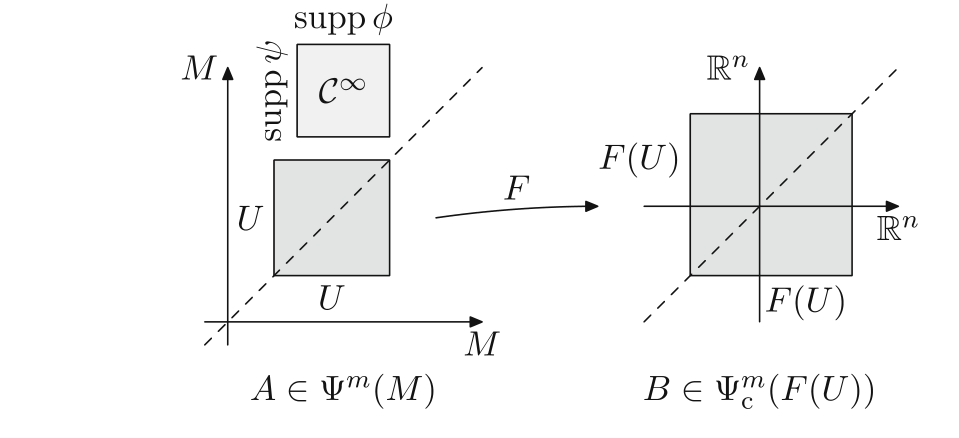
\includegraphics[width=0.72\textwidth]{figs/fig5_2_clean.png}
    \caption{流形上伪微分算子通过坐标卡局域化与对角线外光滑余核的定义分解示意.}
    \label{fig:5.2}
\end{figure}

\begin{remark}[流形 $\R^n$ 上的算子类与一致算子类的对比]\label{rem:5.22}
取光滑流形 $M = \R^n$, 则此处定义的 $\Psi^m(M)$ 远远大于第~\ref{ch:04}~章中定义的一致伪微分算子空间 $\Psi^m(\R^n)$. (一个原因是: 我们并不限制 Schwartz 核在对角线 $\operatorname{diag}_M = \{(p, p) : p \in M\}$ 之外的大小.) 为避免混淆, 后者应当记为 $\Psi_\infty^m(\R^n)$. 在本书中处理 $\R^n$ 时, 我们将只使用一致代数中的算子; 因此我们略去下标 ``$\infty$''.
\end{remark}

\begin{remark}[残余算子空间]\label{rem:5.23}
由定义直接看出, 空间 $\Psi^{-\infty}(M)$ 由所有具有 Schwartz 核 $K \in \mathcal{C}^\infty(M^2; \Omega_R)$ 的算子组成. 等价地, $\Psi^{-\infty}(M)$ 是所有有界线性算子 $\mathscr{E}'(M) \to \mathcal{C}^\infty(M)$ 的空间.
\end{remark}

\begin{remark}[局部凸 Fréchet 拓扑]\label{rem:5.24}
在这一点上我们已经可以通过取式~\eqref{eq:5.56a} 与式~\eqref{eq:5.56b} 中出现的所有 $B$ 与 $K$ 的半范数, 在 $\Psi^m(M)$ 上赋予一个局部凸拓扑. 此时 $\Psi^m(M)$ 是完备的(习题~\ref{ex:5.17}). 定理~\ref{thm:5.29} 蕴含: 只需取式~\eqref{eq:5.56a} 中来自某个局部有限开覆盖 (因而特别是可数的) 以及相应截断函数 $\psi$ 的算子 $B$ 的半范数即可; 从而 $\Psi^m(M)$ 事实上是一个 Fr\'echet 空间.
\end{remark}

\begin{example}[Laplace 算子的逆]\label{eg:5.25}
设 $M = \R^n$, $n \neq 2$. 则由 Schwartz 核 $K(x, y) = |x - y|^{-n+2} |\dd y|$ 定义的算子 $A$ 是 $\Psi^{-2}(M)$ 中的元素. (这不是 $\R^n$ 上的一致伪微分算子.) 在例~\ref{eg:4.31} 的记号下, 我们有 $\Delta \circ A = c_n^{-1} I$. 相关的例子在式~\eqref{eq:5.127} 之后以及命题~\ref{prop:5.53} 中讨论.
\end{example}

\begin{example}[圆周 $\mathbb{S}^1$ 上的非微分伪微分算子]\label{eg:5.26}
在 $\mathbb{S}^1 = \R_\theta / 2\pi\mathbb{Z}$ 上, 函数
\begin{equation}\label{eq:5.57}
    f(\theta) \defeq -\frac{1}{2} |\sinh \theta| + \frac{\frac{1}{2} \sinh(2\pi)}{\cosh(2\pi) - 1} \cosh \theta, \qquad \theta \in (-\pi, \pi],
\end{equation}
的 $2\pi$-周期延拓给出的卷积算子满足 $A \in \Psi^{-2}(\mathbb{S}^1)$, 且 $(D_\theta^2 + 1) \circ A = I$.
\end{example}

流形上非微分算子的更多伪微分算子例子在习题~\ref{ex:5.19}, \ref{ex:5.22}, \ref{ex:5.23}, \ref{ex:5.24} 与 \ref{ex:5.25} 中讨论 (后者极大地推广了例~\ref{eg:5.26}).

伪微分算子作用在具紧支集的分布上. 我们在此给出一个直接证明, 而把基于对偶性 (与式~\eqref{eq:4.32} 精神一致) 的``更好''的证明推迟到推论~\ref{cor:5.45}.

\begin{proposition}[伪微分算子在紧支分布上的有界性]\label{prop:5.27}
设 $A \in \Psi^m(M)$. 则 $A$ 从 $\mathcal{C}_{\mathrm{c}}^\infty(M)$ 连续延拓为有界线性算子:
\begin{equation}\label{eq:5.58}
    A \colon \mathscr{E}'(M) \to \Distr(M).
\end{equation}
\end{proposition}

\begin{proof}
固定从属于局部有限紧坐标图册开覆盖 $F_i \colon U_i \to F_i(U_i) \subset \R^n$ 的单位分解 $\{\phi_i\} \subset \SmoothComp(U_i)$. 固定 $\tilde{\phi}_i \in \SmoothComp(U_i)$ 满足在 $\supp \phi_i$ 附近 $\tilde{\phi}_i \equiv 1$. 由条件式~\eqref{eq:5.56a}, 我们可以写出
\begin{equation}\label{eq:5.59}
    \tilde{\phi}_i A \phi_i = \tilde{\phi}_i A \tilde{\phi}_i \phi_i = F_i^* B_i (F_i^{-1})^* \phi_i, \qquad B_i \in \Psi_{\mathrm{c}}^m(F_i(U_i)).
\end{equation}
现在设 $u \in \mathscr{E}'(M)$, 则仅对有限个 $i$ 有 $\phi_i u \neq 0$. 于是我们令
\begin{equation}\label{eq:5.60}
    \tilde{A} u \defeq \sum_i F_i^* B_i (F_i^{-1})^* (\phi_i u) + \sum_i (1 - \tilde{\phi}_i) A (\phi_i u).
\end{equation}
第一个和式中有限个非零求和项的每一项, 都是 $\R^n$ 上具有紧支集的缓增分布的拉回, 因而属于 $\mathscr{E}'(M)$. 第二个有限和根据式~\eqref{eq:5.56b} 属于 $\mathcal{C}^\infty(M)$. 对 $u \in \SmoothComp(M)$, 显然 $\tilde{A} u = A u$. 由 $\SmoothComp(M) \subset \mathscr{E}'(M)$ 的稠密性, 式~\eqref{eq:5.60} 定义了 $A$ 到 $\mathscr{E}'(M)$ 上的唯一连续延拓.
\end{proof}

\begin{lemma}[坐标卡内构造伪微分算子]\label{lem:5.28}
设 $M$ 为 $n$ 维流形, 设 $F \colon U \to F(U) \subset \R^n$ 为局部坐标卡. 若 $B \in \Psi_{\mathrm{c}}^m(F(U)) \subset \Psi^m(\R^n)$, 则由
\begin{equation}\label{eq:5.61}
    A u \defeq F^* B (F^{-1})^* (u|_U), \qquad u \in \SmoothComp(M)
\end{equation}
在 $U$ 上定义且在 $M \setminus U$ 上令 $A u \defeq 0$ 的算子 $A \colon \SmoothComp(M) \to \mathcal{C}^\infty(M)$ 确立为一个元素 $A \in \Psi^m(M)$.
\end{lemma}

这已经说明 $M$ 上存在大量的伪微分算子, 即形如式~\eqref{eq:5.61} 的算子的局部有限和. 这给出了 $\Psi^m(M)$ 中几乎全部的元素 (即相差一个具光滑积分核的算子).

\begin{proof}
我们首先验证式~\eqref{eq:5.56a}. 设 $G \colon V \to G(V) \subset \R^n$ 为另一个局部坐标卡, 设 $\chi \in \SmoothComp(M)$, $\supp\chi \subset V$. 则
\begin{equation}\label{eq:5.62}
    B_1 \defeq ((F^{-1})^* \chi) B ((F^{-1})^* \chi) \in \Psi_{\mathrm{c}}^m(F(U \cap V)).
\end{equation}
记坐标变换为 $\kappa \defeq F \circ G^{-1} \colon G(U \cap V) \to F(U \cap V)$; 则由定理~\ref{thm:5.2},
\begin{equation}\label{eq:5.63}
    B_2 \defeq (B_1)_\kappa = \kappa^* B_1 (\kappa^{-1})^* \in \Psi_{\mathrm{c}}^m(G(U \cap V)).
\end{equation}
因此
\begin{equation}\label{eq:5.64}
    \chi A(\chi u) = F^* B_1 (F^{-1})^* u|_{U \cap V} = G^* \kappa^* B_1 (\kappa^{-1})^* (G^{-1})^* u|_{U \cap V} = G^* B_2 (G^{-1})^* u|_{U \cap V},
\end{equation}
满足所求条件.

关于式~\eqref{eq:5.56b}: 给定 $\phi, \psi \in \mathcal{C}^\infty(M)$ 满足 $\supp\phi \cap \supp\psi = \emptyset$, 对 $u \in \SmoothComp(M)$,
\begin{equation}\label{eq:5.65}
    \phi A(\psi u) = F^* B' (F^{-1})^* (u|_U), \qquad B' \defeq ((F^{-1})^* \phi) B ((F^{-1})^* \psi) \in \Psi_{\mathrm{c}}^{-\infty}(F(U)) \subset \Psi^{-\infty}(\R^n),
\end{equation}
其中使用了 $\supp((F^{-1})^* \phi) \cap \supp((F^{-1})^* \psi) = \emptyset$. 由于 $B'$ 的 Schwartz 核是光滑的, 即证得式~\eqref{eq:5.56b}.
\end{proof}

\begin{theorem}[通过坐标图册刻画伪微分算子]\label{thm:5.29}
设 $M$ 为 $n$ 维流形, 设 $M = \bigcup_i U_i$ 为满足 $\bar{U}_i$ 紧致的局部有限坐标卡开覆盖 $F_i \colon U_i \to F_i(U_i) \subset \R^n$. 设 $A \colon \SmoothComp(M) \to \Distr(M)$ 为线性算子. 则 $A \in \Psi^m(M)$ 当且仅当存在算子 $B_i \in \Psi_{\mathrm{c}}^m(F_i(U_i))$ 与截面 $K \in \mathcal{C}^\infty(M^2; \Omega_R)$ 使得
\begin{equation}\label{eq:5.66}
    A = K + \sum_i F_i^* B_i (F_i^{-1})^*
\end{equation}
(在此我们将算子与其 Schwartz 核等同视之).
\end{theorem}

\begin{proof}
若 $A$ 具有式~\eqref{eq:5.66} 的形式, 则由引理~\ref{lem:5.28} $A \in \Psi^m(M)$. 反之, 设 $A \in \Psi^m(M)$. 设 $\{\phi_i\} \subset \SmoothComp(U_i)$ 为从属于 $\{U_i\}$ 的单位分解, 即 $\supp\phi_i \subset U_i$ 且 $\sum_i \phi_i(x) = 1$ ($\forall\,x \in M$). 选取 $\tilde{\phi}_i \in \SmoothComp(U_i)$ 满足 $\supp\tilde{\phi}_i \subset U_i$ 且在 $\supp\phi_i$ 附近 $\tilde{\phi}_i \equiv 1$. 对 $u \in \SmoothComp(M)$, 我们有
\begin{equation}\label{eq:5.67}
    A u = \sum_i \tilde{\phi}_i A \phi_i u + \sum_i (1 - \tilde{\phi}_i) A \phi_i u.
\end{equation}
根据定义, $(1 - \tilde{\phi}_i) A \phi_i$ 具有光滑 Schwartz 核 $K_i \in \mathcal{C}^\infty(M^2; \Omega_R)$; 由于 $\supp K_i$ 是局部有限的, 我们可以定义
\begin{equation}\label{eq:5.68}
    K \defeq \sum_i K_i \in \mathcal{C}^\infty(M^2; \Omega_R).
\end{equation}
考察式~\eqref{eq:5.67} 第一项求和中的项 $\tilde{\phi}_i A \phi_i$, 注意到
\begin{equation}\label{eq:5.69}
    \tilde{\phi}_i A(\phi_i u) = \tilde{\phi}_i A \tilde{\phi}_i (\phi_i u).
\end{equation}
但 $\tilde{\phi}_i A \tilde{\phi}_i = F_i^* B'_i (F_i^{-1})^*$ (其中 $B'_i \in \Psi_{\mathrm{c}}^m(F_i(U_i))$), 因此
\begin{equation}\label{eq:5.70}
    \tilde{\phi}_i A \phi_i = F_i^* B_i (F_i^{-1})^*, \qquad B_i v \defeq B'_i \left( ((F_i^{-1})^* \phi_i) v \right), \quad v \in \SmoothComp(F_i(U_i)),
\end{equation}
其中 $B_i \in \Psi_{\mathrm{c}}^m(F_i(U_i))$. 证毕.
\end{proof}

当 $M$ 不紧致时, 一般而言无法复合两个伪微分算子, 即使两者阶数都是 $-\infty$; 因为它们只作用在 $\SmoothComp(M)$ 上, 而一般并不作用在 $\mathcal{C}^\infty(M)$ 上, 问题在于 Schwartz 核在对角线之外可能增长. 最简单的补救办法是对 Schwartz 核附加一个额外假设:

\begin{definition}[适正支集伪微分算子]\label{def:5.30}
若算子 $A \in \Psi^m(M)$ 的 Schwartz 核 $K \in \mathcal{D}'(M^2; \Omega_R)$ 在向左, 右两因子的投影映射 $\pi_L \colon \supp K \to M$ 与 $\pi_R \colon \supp K \to M$ 下均为适正映射 (即紧集的原像仍为紧集), 则称 $A$ 为\textbf{适正支集的} (properly supported).
\end{definition}

紧流形上的每个伪微分算子都是适正支集的. 在一般流形上, 每个伪微分算子都是一个适正支集算子与一个残余算子之和 (习题~\ref{ex:5.16}). 因此在人们不关心 $-\infty$ 阶误差的情形下, 可以完全只使用适正支集的算子.

于是, 适正支集算子在 $\SmoothComp(M)$ 与 $\mathscr{E}'(M)$ 上是有界的. 借助单位分解论证可以说明它们在 $\mathcal{C}^\infty(M)$ 与 $\Distr(M)$ 上也是有界的; 使用对偶性论证的证明见推论~\ref{cor:5.45}. 适正支集的残余算子把 $\Distr(M)$ 映到 $\mathcal{C}^\infty(M)$, 把 $\mathscr{E}'(M)$ 映到 $\SmoothComp(M)$.

\begin{remark}[流形 $\R^n$ 上的适正支集算子与一致算子]\label{rem:5.31}
补充注记~\ref{rem:5.22}: 当 $M = \R^n$ 时, 由适正支集算子组成的子空间与一致伪微分算子空间 $\Psi_\infty^m(\R^n)$ 之间不存在简单的包含关系: 一方面, $\Psi_\infty^m(\R^n)$ 中元素的 Schwartz 核在 $\R^n \times \R^n$ 中可以具有全空间支集, 因而并非适正支集的; 另一方面, $\Psi^m(M)$ 中的适正支集元素亦不必然属于 $\Psi_\infty^m(\R^n)$, 因为后者的属于性要求在对角线外部具有一致衰减界 (对比推论~\ref{cor:4.9}).
\end{remark}

\begin{theorem}[流形上伪微分算子的复合定理]\label{thm:5.32}
设 $A \in \Psi^m(M)$, $B \in \Psi^{m'}(M)$, 且假定 $A, B$ 中至少有一个算子是适正支集的. 则复合算子 $A \circ B \colon \mathcal{C}_{\mathrm{c}}^\infty(M) \to \mathcal{C}^\infty(M)$ 是良定义的伪微分算子: $A \circ B \in \Psi^{m+m'}(M)$. 若 $A, B$ 均为适正支集的, 则 $A \circ B$ 亦为适正支集的.
\end{theorem}

在证明中, 我们将对一类特殊的开覆盖使用定理~\ref{thm:5.29} 的刻画:

\begin{lemma}[特殊坐标覆盖]\label{lem:5.33}
设 $M$ 为光滑流形. 存在 $M$ 的局部有限开覆盖 $\{U_i\}$, 使得只要 $U_i \cap U_j \neq \emptyset$, 就必定存在包含 $U_i \cup U_j$ 的局部坐标卡 $F \colon U \to F(U) \subset \R^n$ (即 $U \supset U_i \cup U_j$).
\end{lemma}

\begin{proof}
流形 $M$ 是可度量化的 (这由 Urysohn 度量化定理或 Riemann 几何直接保证). 用 $d$ 表示 $M$ 上的一个固定度量, 记度量球为 $B(p, r) \defeq \{q \in M : d(p, q) < r\}$. 对每个 $p \in M$, 令
\begin{equation}\label{eq:5.71}
    r_0(p) \defeq \sup \left\{ r \in [0, 1] : B(p, r) \text{ 包含在某个局部坐标卡内} \right\}.
\end{equation}
由于 $M$ 是流形, 对所有 $p \in M$ 均有 $r_0(p) > 0$. 对 $p \in M$, 定义开集
\begin{equation}\label{eq:5.72}
    V_p \defeq B\left( p, \frac{r_0(p)}{10} \right).
\end{equation}
假定 $V_p \cap V_q \neq \emptyset$, 则 $d(p, q) \le \frac{1}{10}(r_0(p) + r_0(q)) \le \frac{1}{5} \max(r_0(p), r_0(q))$. 由对称性不妨设 $r_0(p) \ge r_0(q)$. 若 $z \in V_p \cup V_q$, 则
\begin{equation}\label{eq:5.73}
    d(p, z) < \max\left( \frac{r_0(p)}{10}, d(p, q) + \frac{r_0(q)}{10} \right) \le \max\left( \frac{r_0(p)}{10}, \frac{r_0(p)}{5} + \frac{r_0(p)}{10} \right) < \frac{r_0(p)}{2}.
\end{equation}
因此 $V_p \cup V_q \subset B(p, \frac{r_0(p)}{2})$ 整体包含在同一个坐标卡内. 开覆盖 $\{V_p : p \in M\}$ 的任意局部有限加细 $\{U_i\}$ 即满足所求条件 (见图~\ref{fig:5.3}).
\end{proof}

\begin{figure}[htbp]
    \centering
    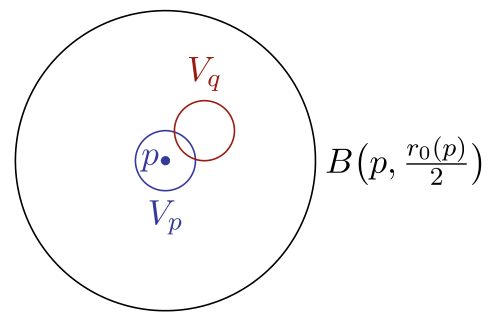
\includegraphics[width=0.48\textwidth]{figs/fig5_3_clean.png}
    \caption{流形坐标覆盖下邻域两两相交时的几何度量与支撑相容性.}
    \label{fig:5.3}
\end{figure}

\begin{proof}[定理~\ref{thm:5.32} 的证明]
由引理~\ref{lem:5.33}, 我们可以固定一个由满足 $\bar{U}_i$ 紧致的坐标卡 $F_i \colon U_i \to F_i(U_i) \subset \R^n$ 构成的开覆盖 $M = \bigcup_i U_i$, 使得只要 $U_i \cap U_j \neq \emptyset$, 并集 $U_i \cup U_j$ 就包含于某个坐标卡 $F_{ij} \colon U_{ij} \to F_{ij}(U_{ij}) \subset \R^n$ 之内.

假定 $A$ 是适正支集的. (若 $B$ 是适正支集的则论证完全对称.) 写出
\begin{equation}\label{eq:5.74}
    \begin{aligned}
        A &= K + \sum_i F_i^* A_i (F_i^{-1})^*, \qquad A_i \in \Psi_{\mathrm{c}}^m(F_i(U_i)), \quad K \in \mathcal{C}^\infty(M^2; \Omega_R), \\
        B &= K' + \sum_i F_i^* B_i (F_i^{-1})^*, \qquad B_i \in \Psi_{\mathrm{c}}^{m'}(F_i(U_i)), \quad K' \in \mathcal{C}^\infty(M^2; \Omega_R).
    \end{aligned}
\end{equation}
由于 $A$ 与所有的 $F_i^* A_i (F_i^{-1})^*$ 都是适正支集的, $K$ 亦为适正支集的. 逐项考察复合算子 $A \circ B$, 并追踪各分量 Schwartz 核的支集:

首先证明 $K \circ K' \in \Psi^{-\infty}(M)$. 我们有 $(K \circ K')(x, y) = \int_M K(x, z) K'(z, y)$. 对任意紧集 $K_1 \subset M$, 存在紧集 $K_2 \subset M$ (具体而言可取 $K_2 = \pi_R(\supp K \cap \pi_L^{-1}(K_1))$) 使得
\begin{equation}\label{eq:5.75}
    (K \circ K')(x, y) = \int_{K_2} K(x, z) K'(z, y), \qquad x \in K_1.
\end{equation}
因此 $K \circ K'$ 的 Schwartz 核属于 $\mathcal{C}^\infty(M^2; \Omega_R)$.

接着考察复合 $K_i \defeq K \circ F_i^* B_i (F_i^{-1})^*$. 它将 $u \in \mathscr{E}'(M)$ 映入 $\mathcal{C}^\infty(M)$; 且若 $\supp u \cap U_i = \emptyset$, 则 $K_i u = 0$. 于是由注记~\ref{rem:5.23},
\begin{equation}\label{eq:5.76}
    K_i \in \mathcal{C}^\infty(M^2; \Omega_R), \qquad \supp K_i \subset M \times U_i.
\end{equation}
类似地可证明
\begin{equation}\label{eq:5.77}
    K'_i \defeq F_i^* A_i (F_i^{-1})^* \circ K' \in \mathcal{C}^\infty(M^2; \Omega_R), \qquad \supp K'_i \subset U_i \times M.
\end{equation}
最后, 我们需要考察复合
\begin{equation}\label{eq:5.78}
    C_{ij} \defeq F_i^* A_i (F_i^{-1})^* \circ F_j^* B_j (F_j^{-1})^* \colon \SmoothComp(M) \to \mathcal{C}^\infty(M).
\end{equation}
当 $U_i \cap U_j = \emptyset$ 时, 该复合格外为 0. 当 $U_i \cap U_j \neq \emptyset$ 时, 由引理~\ref{lem:5.28}, 我们可将式~\eqref{eq:5.78} 等价写为
\begin{equation}\label{eq:5.79}
    F_{ij}^* A_{ij} (F_{ij}^{-1})^* \circ F_{ij}^* B_{ij} (F_{ij}^{-1})^* = F_{ij}^* (A_{ij} \circ B_{ij}) (F_{ij}^{-1})^*,
\end{equation}
其中 $A_{ij} \in \Psi_{\mathrm{c}}^m(F_{ij}(U_{ij}))$ 且 $B_{ij} \in \Psi_{\mathrm{c}}^{m'}(F_{ij}(U_{ij}))$. 由 $\R^n$ 上的复合定理 (定理~\ref{thm:4.22}), $A_{ij} \circ B_{ij} \in \Psi_{\mathrm{c}}^{m+m'}(F_{ij}(U_{ij}))$. 综上所述, $A \circ B \in \Psi^{m+m'}(M)$, 且当 $A, B$ 均是适正支集时其复合显然保持适正支集.
\end{proof}

\begin{corollary}[紧流形上的复合]\label{cor:5.34}
若 $M$ 为紧流形, 则 $\Psi^m(M) \circ \Psi^{m'}(M) \subset \Psi^{m+m'}(M)$.
\end{corollary}

\section{主符号}\label{sec:5.5}
\index{liuxingshang zhufuhao@流形上的主符号 (principal symbols on manifolds)}%

定理~\ref{thm:5.2} 中公式~\eqref{eq:5.2} 的精髓在于: 动量变量 $\xi$ 变换时所乘的逆转置矩阵 $(\kappa'(x)^T)^{-1}$, 恰恰是余切丛 $T^* M$ 在底流形坐标变换下余切向量的严格拉回变换法则! 这从根本上揭示出: 伪微分算子的主符号天生是定义在余切丛 $T^* M$ 上的几何对象.

\begin{definition}[向量丛上的符号空间]\label{def:5.35}
设 $\pi \colon E \to M$ 为秩为 $k$ 的光滑向量丛. 对 $m \in \R$, 符号空间 $S^m(E) \subset \mathcal{C}^\infty(E)$ 由所有满足如下条件的函数 $a \in \mathcal{C}^\infty(E)$ 组成: 在局部平凡化卡 $\tau \colon \pi^{-1}(U) \to F(U) \times \R^k$ 下,
\begin{equation}\label{eq:5.80}
    b(x, v) \defeq (\tau^{-1})^* (a|_{\pi^{-1}(U)})(x, v) \in \mathcal{C}^\infty(F(U) \times \R^k),
\end{equation}
且对任意 $\phi \in \SmoothComp(F(U))$, 均有 $\phi(x) b(x, v) \in S^m(\R^n; \R^k)$. 当 $E = T^* M$ 时, 我们得到余切丛上的符号空间 $S^m(T^* M)$.
\end{definition}

\begin{lemma}[坐标卡内定义的符号延拓]\label{lem:5.36}
在定义~\ref{def:5.35} 的记号下, 若 $\phi \in \SmoothComp(F(U))$, $b \in S^m(\R^n; \R^k)$, 则 $a \defeq \tau^*(\phi b) \in S^m(E)$.
\end{lemma}

\begin{proof}
在另一个坐标卡与平凡化下, 转变函数表达为
\begin{equation}\label{eq:5.81}
    b'(x, v) = \phi(\kappa(x)) b(\kappa(x), \Phi(x) v), \qquad x \in F'(U \cap U'),
\end{equation}
其中 $\kappa \defeq F \circ (F')^{-1} \colon F'(U \cap U') \to F(U \cap U')$, 且 $\Phi \colon F'(U \cap U') \to \mathrm{GL}(k, \R)$ 为光滑映射. 设 $\psi \in \SmoothComp(F'(U'))$, 则 $\chi(x) \defeq \psi(x) \phi(\kappa(x)) \in \SmoothComp(F'(U \cap U'))$. 我们需要验证
\begin{equation}\label{eq:5.82}
    \chi(x) b(\kappa(x), \Phi(x) v) \in S^m(\R^n; \R^k).
\end{equation}
这直接遵循式~\eqref{eq:5.14} 的完全同类求导计算.
\end{proof}

\begin{corollary}[通过坐标卡刻画符号空间]\label{cor:5.37}
设 $M = \bigcup_i U_i$ 为满足 $\bar{U}_i$ 紧致的局部有限坐标卡开覆盖, $\tau_i$ 为局部平凡化. 则 $a \in \mathcal{C}^\infty(E)$ 属于 $S^m(E)$ 当且仅当存在符号 $b_i \in S^m(\R^n; \R^k)$ 与 $\chi_i \in \SmoothComp(F_i(U_i))$ 使得
\begin{equation}\label{eq:5.83}
    a = \sum_i \tau_i^* (\chi_i b_i).
\end{equation}
\end{corollary}

现在, 给定算子 $A \in \Psi^m(M)$, 我们期望其主符号是商空间 $S^m(T^* M) / S^{m-1}(T^* M)$ 中的元素. 我们首先在局部进行定义: 设 $F \colon U \to F(U) \subset \R^n$ 为局部坐标卡且 $\bar{U}$ 紧致, 设开集 $V \subset U$ 满足 $\bar{V} \subset U$. 记 $\tau \colon T_U^* M \to F(U) \times \R^n$ 为由 $F$ 诱导的平凡化. 选取切断函数 $\chi \in \SmoothComp(U)$ 满足在 $\bar{V}$ 上 $\chi \equiv 1$. 则我们置
\begin{equation}\label{eq:5.84}
    a_V \defeq \left. \tau^*\left( \sigma_L((F^{-1})^* \chi A \chi F^*) \right) \right|_{T_V^* M} \in S^m(T_V^* M).
\end{equation}
由欧氏空间上的局部理论 (特别是定理~\ref{thm:5.2}), 等价类
\begin{equation}\label{eq:5.85}
    [a_V] \in S^m(T_V^* M) / S^{m-1}(T_V^* M)
\end{equation}
与 $\chi$ 的选取以及覆盖 $\bar{V}$ 邻域的坐标系 $F$ 的选取均无关. 此外, 若 $V' \subset V$, 则限制到 $V'$ 满足 $[a_V]|_{V'} = [a_{V'}]$.

\begin{definition}[流形上伪微分算子的主符号]\label{def:5.38}
算子 $A \in \Psi^m(M)$ 的\textbf{主符号}是唯一满足如下性质的元素
\begin{equation}\label{eq:5.86}
    \sigma_m(A) \in S^m(T^* M) / S^{m-1}(T^* M):
\end{equation}
若 $a \in S^m(T^* M)$ 为 $\sigma_m(A)$ 的任意代表元且 $V$ 如上, 则 $[a|_{T_V^* M}] = [a_V] \in S^m(T_V^* M) / S^{m-1}(T_V^* M)$.
\end{definition}

该定义蕴含了主符号 $\sigma_m(A)$ 存在且唯一的断言. 存在性由 $[a_V]$ 的相容性质直接得出: 选取开覆盖 $\{V\}$ 的局部有限子覆盖 $\{V_i\}$ 及其从属单位分解 $\{\phi_i\}$, 由推论~\ref{cor:5.37} $a \defeq \sum_i \phi_i a_{V_i} \in S^m(T^* M)$; 我们随后令
\begin{equation}\label{eq:5.87}
    \sigma_m(A) \defeq [a].
\end{equation}
对任意开集 $V$ 及 $\phi \in \SmoothComp(V)$, 在 $V$ 上有
\begin{equation}\label{eq:5.88}
    \phi a = \sum_i \tilde{\phi}_i (\phi_i \phi a_{V_i}) = \sum_i \tilde{\phi}_i (\phi_i \phi a_V + e_i) = \phi a_V + \sum_i \tilde{\phi}_i e_i,
\end{equation}
其中 $\sum_i \tilde{\phi}_i e_i \in S^{m-1}(T^* M)$. 唯一性同理得出.

\begin{proposition}[流形上主符号短正合列]\label{prop:5.39}
主符号映射给出如下短正合列:
\begin{equation}\label{eq:5.89}
    0 \to \Psi^{m-1}(M) \hookrightarrow \Psi^m(M) \xrightarrow{\sigma_m} S^m(T^* M) / S^{m-1}(T^* M) \to 0.
\end{equation}
\end{proposition}

\begin{proof}
我们只需证明 $\sigma_m$ 的满射性. 选取从属于坐标卡开覆盖 $M = \bigcup_i U_i$ ($\bar{U}_i$ 紧致, 坐标映射为 $F_i \colon U_i \to F_i(U_i) \subset \R^n$) 的局部有限单位分解 $\{\phi_i\}$. 将任意给定的 $a \in S^m(T^* M)$ 分解为 $a = \sum_i \phi_i a$. 只需证明存在 Schwartz 核支集包含于 $U_i \times U_i$ 之内的算子 $A_i \in \Psi^m(M)$ 满足 $\sigma_m(A_i) = [\phi_i a]$, 随后即可取局部有限和 $A = \sum_i A_i$. 这很容易做到: 若取 $\tilde{\phi}_i \in \SmoothComp(U_i)$ 满足在 $\supp\phi_i$ 上 $\tilde{\phi}_i \equiv 1$, 则算子
\begin{equation}\label{eq:5.90}
    A_i = F_i^* \Op\left( \left( (F_i^{-1})^* \phi_i \right)(x) a(x, \xi) \left( (F_i^{-1})^* \tilde{\phi}_i \right)(y) \right) (F_i^{-1})^*
\end{equation}
即满足所求条件.
\end{proof}

由欧氏空间上的相应结论 (命题~\ref{prop:4.24}) 立即推出:

\begin{proposition}[主符号的乘法性]\label{prop:5.40}
若 $A \in \Psi^m(M)$, $B \in \Psi^{m'}(M)$, 且其中至少有一个是适正支集的, 则
\begin{equation}\label{eq:5.91}
    \sigma_{m+m'}(A \circ B) = \sigma_m(A) \sigma_{m'}(B).
\end{equation}
\end{proposition}

关于换位子主符号的对等结论 (命题~\ref{prop:4.25}) 将在第~\ref{sec:5.14}~节中讨论.

\section{量化}\label{sec:5.6}
\index{lianghua@量化 (quantization)}%

一般而言, 并不存在一种完全自然的方式将 $T^* M$ 上的符号量化为 $M$ 上的伪微分算子. 然而, 我们有如下极为实用的构造: 固定坐标卡覆盖 $M = \bigcup_i U_i$ (满足 $\bar{U}_i$ 紧致, $F_i \colon U_i \to F_i(U_i) \subset \R^n$) 构成的局部有限开覆盖, 并设 $\{\phi_i\} \subset \SmoothComp(U_i)$ 为从属于 $\{U_i\}$ 的单位分解. 固定 $\tilde{\phi}_i \in \SmoothComp(U_i)$ 使得在 $\supp\phi_i$ 附近 $\tilde{\phi}_i \equiv 1$. 给定 $a \in S^m(T^* M)$, 定义
\begin{equation}\label{eq:5.92}
    \Op(a) \defeq \sum_i F_i^* \Op\left( \left( (F_i^{-1})^* \phi_i \right)(x) \left( (\tau_i^{-1})^* a \right)(x, \xi) \left( (F_i^{-1})^* \tilde{\phi}_i \right)(y) \right) (F_i^{-1})^*,
\end{equation}
其中 $\tau_i \colon T^*_{U_i} M \to F_i(U_i) \times \R^n$ 为由 $F_i$ 诱导的平凡化. 由定理~\ref{thm:5.29}, 式~\eqref{eq:5.92} 定义了映射
\begin{equation}\label{eq:5.93}
    \Op \colon S^m(T^* M) \to \Psi^m(M).
\end{equation}

\begin{proposition}[量化映射的性质]\label{prop:5.41}
式~\eqref{eq:5.93} 中的映射 $\Op$ 是连续线性的, 且取值于适正支集算子组成的子空间中. 我们有 $\Op(1) = I$ (恒等算子). 此外, $\Op \colon S^m(T^* M) \to \Psi^m(M)$ 模去 $\Psi^{-\infty}(M)$ 是满射; 即 $\Psi^m(M) = \Op(S^m(T^* M)) + \Psi^{-\infty}(M)$.
\end{proposition}

\begin{proof}
我们仅给出最后一个断言的证明概要. 在式~\eqref{eq:5.66} 的记号下, 我们可以将任意给定的 $A \in \Psi^m(M)$ 写为 $A \defeq A_m + K$ 的形式, 其中 $A_m = \sum_i F_i^* B_i (F_i^{-1})^*$, 且 $K \in \Psi^{-\infty}(M)$. 我们将算子 $B_i \in \Psi_{\mathrm{c}}^m(F_i(U_i))$ 的符号沿着平凡化 $\tau_i$ 的拉回求和, 得到符号 $a_m \in S^m(T^* M)$; 由主符号的坐标不变性可知,
\begin{equation}\label{eq:5.94}
    A_{m-1} \defeq A_m - \Op(a_m) \in \Psi^{m-1}(M).
\end{equation}
随后我们可将定理~\ref{thm:5.29} 应用于 $A_{m-1}$. 归纳论证由此产生 $a_{m-j} \in S^{m-j}(T^* M)$ ($j \in \N$), 使得 $A_{m-j-1} \defeq A_{m-j} - \Op(a_{m-j}) \in \Psi^{m-j-1}(M)$. 取 $a \in S^m(T^* M)$ 为 $a_{m-j}$ ($j \in \N_0$) 的渐近和, 我们最终得到
\begin{equation}\label{eq:5.95}
    A = A_m + K = \Op(a) + K + R, \qquad R \in \Psi^{-\infty}(M).
\end{equation}
其中 $K + R$ 是光滑的残余算子.
\end{proof}

\section{作用在向量丛截面上的算子}\label{sec:5.7}
\index{xiangliangcong@向量丛截面算子 (operators on sections)}%

读者可能会问, 为什么我们迄今为止尚未讨论 $A \in \Psi^m(M)$ (甚至 $A \in \Diff^m(M)$) 的伴随算子. 由于我们并没有一种在流形 $M$ 上积分函数的内在不变方式, 定义 $A^*$ 唯一合理的方式是通过
\begin{equation}\label{eq:5.96}
    \int_M (A u)(x) \overline{v(x)} = \int_M u(x) \overline{A^* v(x)}, \qquad u \in \SmoothComp(M), \quad v \in \SmoothComp(M; \Omega M);
\end{equation}
换言之, $A^*$ 应当是一个作用在 $1$-密度上的算子. 我们将把将 $E$ 的截面映为 $F$ 的截面的 $m$ 阶微分算子空间 $\Diff^m(M; E, F)$ 的定义留给读者作为练习, 直接进入伪微分算子的情形.

\begin{definition}[作用在向量丛截面上的伪微分算子]\label{def:5.42}
设 $M$ 为光滑流形, $\pi_E \colon E \to M$ 与 $\pi_F \colon F \to M$ 为秩分别为 $k_E, k_F$ 的两个实向量丛 (复向量丛的情形完全对等). 则 $\Psi^m(M; E, F)$ 是所有满足如下性质的线性算子
\begin{equation}\label{eq:5.97}
    A \colon \SmoothComp(M; E) \to \Smooth(M; F)
\end{equation}
构成的空间:
\begin{enumerate}
    \item 设 $U \subset M$ 为任意开集, $G \colon U \to G(U) \subset \R^n$ 为微分同胚, 且设 $\tau_E \colon \pi_E^{-1}(U) \to G(U) \times \R^{k_E}$, $\tau_F \colon \pi_F^{-1}(U) \to G(U) \times \R^{k_F}$ 为 $E, F$ 的局部平凡化. 利用 $\tau_E$, 将 $E$ 在 $U$ 上的光滑截面等同于 $U$ 上的光滑函数 $k_E$-元组, 对 $F$ 的截面亦然. 若 $\psi \in \SmoothComp(U)$, 则存在一个伪微分算子的 $k_F \times k_E$ 矩阵 $B = (B_{ij})$, 其中 $B_{ij} \in \Psi_{\mathrm{c}}^m(G(U))$, 使得在 $U$ 上有
    \begin{equation}\label{eq:5.98}
        (\psi A(\psi u))_i = \sum_{j=1}^{k_E} G^* \left( B_{ij} ((G^{-1})^* u)_j \right), \qquad u \in \SmoothComp(M; E), \quad i = 1, \ldots, k_F.
    \end{equation}
    \item 若 $\phi, \psi \in \Smooth(M)$ 满足 $\supp\phi \cap \supp\psi = \emptyset$, 则存在光滑核 $K \in \Smooth(M^2; \pi_L^* F \otimes \pi_R^*(E^* \otimes \Omega M))$ 使得 $\phi A \psi = K$.
\end{enumerate}
在 $F = E$ 的特例下, 我们记 $\Psi^m(M; E) \defeq \Psi^m(M; E, E)$.
\end{definition}

在局部坐标与平凡化下, 算子 $A \in \Psi^m(M; E, F)$ 的符号是以 $\R^{k_E} \to \R^{k_F}$ 的线性映射为取值的符号. 其内在不变定义如下: 记 $\pi \colon T^* M \to M$ 为投影. 给定向量丛 $G \to M$, 我们可以考虑其拉回丛 $\pi^* G \to T^* M$ (定义~\ref{def:5.9}); $G$ 在开集 $U \subset M$ 上的平凡化 $G|_U \cong U \times \R^{k_G}$, 在 $T^*_U M$ 上诱导了在 ``$T^* M$ 纤维上常值'' 的拉回丛平凡化:
\begin{equation}\label{eq:5.99}
    (\pi^* G)|_{T^*_U M} \cong T^* U \times \R^{k_G},
\end{equation}
即通过局部平凡化等同 $(\pi^* G)_{(x, \xi)} = G_x \cong \R^{k_G}$. 我们随后用
\begin{equation}\label{eq:5.100}
    S^m(T^* M; \pi^* G) \subset \Smooth(T^* M; \pi^* G)
\end{equation}
表示所有在局部坐标以及 $G$ 的平凡化下 (该平凡化如式~\eqref{eq:5.99} 般诱导了 $\pi^* G$ 的平凡化) 呈现为 $\R^n$ 上 $m$ 阶符号的 $k_G$-向量的光滑截面空间. 内在地,
\begin{equation}\label{eq:5.101}
    \sigma_m(A) \in (S^m / S^{m-1})(T^* M; \pi^* \mathrm{Hom}(E, F)).
\end{equation}
这意味着 $\sigma_m(A)$ 的一个代表元是一个将每个 $(x, \xi) \in T^* M$ 映为 $\mathrm{Hom}(E_x, F_x)$ 中元素的映射. 我们有短正合列:
\begin{equation}\label{eq:5.102}
    0 \to \Psi^{m-1}(M; E, F) \hookrightarrow \Psi^m(M; E, F) \xrightarrow{\sigma_m} (S^m / S^{m-1})(T^* M; \pi^* \mathrm{Hom}(E, F)) \to 0.
\end{equation}

第~\ref{sec:5.4}--\ref{sec:5.5}~节中的结论完全延拓至此; 此外, 我们还可以定义伴随算子:

\begin{proposition}[复合与伴随]\label{prop:5.43}
设 $M$ 为光滑流形, $E, F, G \to M$ 为三个向量丛.
\begin{enumerate}
    \item 设 $A \in \Psi^m(M; F, G)$, $B \in \Psi^{m'}(M; E, F)$, 且其中至少有一个是适正支集的. 则 $A \circ B \in \Psi^{m+m'}(M; E, G)$, 且 $\sigma_{m+m'}(A \circ B) = \sigma_m(A) \circ \sigma_{m'}(B)$.
    \item 设 $A \in \Psi^m(M; E, F)$. 则其 (实) 伴随算子 $A^T$ 通过
    \begin{equation}\label{eq:5.103}
        \int_M (A u) v = \int_M u (A^T v), \qquad u \in \SmoothComp(M; E), \quad v \in \SmoothComp(M; F^* \otimes \Omega M)
    \end{equation}
    定义, 是一个伪微分算子:
    \begin{equation}\label{eq:5.104}
        A^T \in \Psi^m(M; F^* \otimes \Omega M, E^* \otimes \Omega M),
    \end{equation}
    且满足 $\sigma_m(A^T) = \sigma_m(A)^T$. 若 $A$ 为适正支集的, 则 $A^T$ 亦为适正支集的.
\end{enumerate}
\end{proposition}

\begin{remark}[具备额外结构的向量丛]\label{rem:5.44}
\begin{enumerate}
    \item 若 $E, F$ 为带有反线性对合 (``复共轭'') 的复向量丛, 则可以类似于式~\eqref{eq:5.103} 定义伴随算子 $A^*$, 但在第二个因子上取复共轭; 此时有
    \begin{equation}\label{eq:5.105}
        A^* \in \Psi^m(M; F^* \otimes \Omega M, E^* \otimes \Omega M), \qquad \sigma_m(A^*) = \sigma_m(A)^*.
    \end{equation}
    这特别适用于 $E = F = M \times \mathbb{C}$ 的情形, 此时 $E, F$ 的截面即为 $M$ 上的复数值函数.
    \item $E$ 上的内积诱导了同构 $E^* \cong E$ (当内积为半双线性时该同构为反线性的). 若进一步选取 $\Omega M$ 的一个平凡化, 则 $A^T \in \Psi^m(M; F, E)$ (在复情形下 $A^* \in \Psi^m(M; E, F)$).
\end{enumerate}
\end{remark}

式~\eqref{eq:5.104} 的一个直接推论是如下命题~\ref{prop:5.27} 的推广:

\begin{corollary}[伪微分算子在分布与光滑截面上的作用]\label{cor:5.45}
设 $A \in \Psi^m(M; E, F)$. 则 $A$ 延拓为有界线性算子 $A \colon \mathcal{E}'(M; E) \to \mathcal{D}'(M; F)$. 若 $A$ 是适正支集的, 则 $A$ 还将 $\mathcal{D}'(M; E) \to \mathcal{D}'(M; F)$, 且经限制给出映射 $\Smooth(M; E) \to \Smooth(M; F)$.
\end{corollary}

\begin{proof}
$A^T$ 是有界映射 $\SmoothComp(M; F^* \otimes \Omega M) \to \Smooth(M; E^* \otimes \Omega M)$. 因此我们可以利用式~\eqref{eq:5.104} 通过对偶性定义 $A \colon \mathcal{E}'(M; E) \to \mathcal{D}'(M; F)$; 当限制在 $\SmoothComp(M; E)$ 上时, 它与原算子 $A$ 完全吻合.

若 $A$ 是适正支集的, 则 $A^T$ 将 $\SmoothComp(M; F^* \otimes \Omega M) \to \SmoothComp(M; E^* \otimes \Omega M)$, 从而我们现在可以通过对偶性定义 $A \colon \mathcal{D}'(M; E) \to \mathcal{D}'(M; F)$. 最后注意到 $\Smooth(M; E) \subset \mathcal{D}'(M; E)$; 故只需检验当 $u \in \Smooth(M; E)$ 时 $A u \in \Smooth(M; F)$. 利用紧支单位分解 $1 = \sum_i \phi_i$, 我们有
\begin{equation}\label{eq:5.106}
    A u = A\left( \sum_i \phi_i u \right) = \sum_i A(\phi_i u),
\end{equation}
该式在 $\mathcal{D}'(M; F)$ 中收敛. 由于 $A$ 是适正支集的, 最后的求和是光滑项的局部有限和, 因而其和是光滑截面.
\end{proof}

\section{算子的特殊类别}\label{sec:5.8}
\index{jingdian weifen suanzi@经典伪微分算子 (classical ps.d.o.)}%

设 $M$ 为流形, $E, F \to M$ 为秩为 $k_E, k_F$ 的向量丛.

\begin{definition}[流形上的经典伪微分算子]\label{def:5.46}
设 $m \in \R$. 经典伪微分算子子空间 $\Psi_{\mathrm{cl}}^m(M; E, F) \subset \Psi^m(M; E, F)$ 由所有满足如下条件的算子组成: 其在局部坐标卡以及 $E, F$ 的局部平凡化下的全符号, 是由 $m$ 阶经典符号构成的 $k_F \times k_E$ 矩阵. $\Psi_{\mathrm{cl}}^m(M; E, F)$ 上的主符号映射记录其最高阶齐次部分:
\begin{equation}\label{eq:5.107}
    \sigma_m \colon \Psi_{\mathrm{cl}}^m(M; E, F) \to S_{\mathrm{hom}}^m(T^* M \setminus o; \pi^* \mathrm{Hom}(E, F)).
\end{equation}
\end{definition}

这是一个合理的定义, 因为经典性在局部坐标变换下保持不变; 这直接遵循定理~\ref{thm:5.2} 的证明, 尤其是式~\eqref{eq:5.13}. 读者容易验证两个经典伪微分算子的复合 (其中至少一个是适正支集的) 依然是经典伪微分算子, 且取伴随运算同样保持经典性. 我们有
\begin{equation}\label{eq:5.108}
    \Diff^m(M; E, F) \subset \Psi_{\mathrm{cl}}^m(M; E, F).
\end{equation}

作用在向量丛截面上的算子中一个重要特殊类别如下 (参见例~\ref{eg:5.55}):

\begin{definition}[主标量算子]\label{def:5.47}
设 $m \in \R$ 且 $A \in \Psi^m(M; E)$. 若 $A$ 的主符号在 $E$ 的纤维上是标量乘法, 即存在符号 $a \in S^m(T^* M)$ 使得 $\sigma_m(A)(x, \xi) = a(x, \xi) \mathrm{Id}_{E_x}$, 则称 $A$ 是\textbf{主标量的} (principally scalar).
\end{definition}

\section{紧流形上的椭圆算子与 Fredholm 理论}\label{sec:5.9}
\index{tuoyuan suanzi@椭圆算子 (elliptic operator)}%
\index{Fredholm suanzi@Fredholm 算子 (Fredholm operator)}%
\index{guangyini@广义逆 (generalized inverse)}%

设 $M$ 为无边界 $n$ 维流形, $E, F \to M$ 为两个向量丛.

\begin{definition}[椭圆性]\label{def:5.48}\sloppy
设 $A \in \Psi^m(M; E, F)$, 其主符号记为 $a = \sigma_m(A)$. 若存在符号 $b \in S^{-m}(T^* M; \pi^* \mathrm{Hom}(F, E))$ 使得
\[
    a b - 1 \in S^{-1}(T^* M; \pi^* \mathrm{End}(F)), \qquad b a - 1 \in S^{-1}(T^* M; \pi^* \mathrm{End}(E)),
\]
则称 $A$ 是\textbf{椭圆型的} (elliptic).
\end{definition}

\begin{remark}[椭圆性的等价定义]\label{rem:5.49}
由式~\eqref{eq:4.105} 中的抽象群论论证, 如下定义与 $A$ 的椭圆性等价: 存在符号 $b, b' \in S^{-m}(T^* M; \pi^* \mathrm{Hom}(F, E))$ 使得 $a b - 1 \in S^{-1}(T^* M; \pi^* \mathrm{End}(F))$ 以及 $b' a - 1 \in S^{-1}(T^* M; \pi^* \mathrm{End}(E))$.
\end{remark}

椭圆拟逆构造 (定理~\ref{thm:4.29}) 在此框架下同样成立; 证明留给读者.

\begin{theorem}[椭圆拟逆]\label{thm:5.50}
设 $A \in \Psi^m(M; E, F)$ 是椭圆型的. 则存在适正支集算子 $B \in \Psi^{-m}(M; F, E)$, 在模去 $\Psi^{-\infty}(M; F, E)$ 的意义下唯一, 使得 $A \circ B - I \in \Psi^{-\infty}(M; F)$, $B \circ A - I \in \Psi^{-\infty}(M; E)$. 若 $A$ 是经典的, 则 $B$ 亦为经典的.
\end{theorem}

例~\ref{eg:5.26} 提供了紧流形上椭圆微分算子可逆的一个例子. 不可逆算子具有拟逆的典型例子如下:

\begin{example}[圆周上的导数算子]\label{eg:5.51}
设 $M = \mathbb{S}^1 \defeq \R_\theta / 2\pi\mathbb{Z}$, 并设 $A = D_\theta \in \Psi^1(M)$. 该算子在任何包含非零常数函数的函数空间上均不可逆. $D_\theta$ 在 $\R_\theta$ 上的一个基本解由 $\ii H(\theta)$ 给出. 通过在 $\theta = 0$ 之外进行切断, 可以在 $\mathbb{S}^1$ 上为 $A$ 构造一个拟逆 $B$. 具体而言, 若 $\chi \in \SmoothComp((-\pi, \pi))$ 在 $0$ 附近等于 1, 则我们可以取 $B$ 具有 Schwartz 核
\begin{equation}\label{eq:5.109}
    K_B(\theta, \theta') \defeq -\frac{1}{2} |\theta - \theta'| \chi(\theta - \theta') |\dd\theta'|, \qquad \theta, \theta' \in (-\pi, \pi),
\end{equation}
这是 $\mathcal{D}'(M^2; \Omega_R)$ 的一个元素. 读者可验证这确立了 $B \in \Psi_{\mathrm{cl}}^{-1}(M)$.
\end{example}

\begin{theorem}[紧流形上椭圆伪微分算子的 Fredholm 性质与广义逆]\label{thm:5.52}
设 $M$ 为紧流形, $A \in \Psi^m(M; E, F)$ 为椭圆型算子.
\begin{enumerate}
    \item 算子 $A \colon \Smooth(M; E) \to \Smooth(M; F)$ 是 Fredholm 算子, 即 $\ker A$ 为有限维空间, 且 $\ran A$ 是闭子空间并具有有限余维数. 进一步地,
    \begin{equation}\label{eq:5.110}
        \ran A = \left\{ f \in \Smooth(M; F) : \langle f^*, f \rangle = 0, \; \forall f^* \in \Smooth(M; F^* \otimes \Omega M) \text{ 满足 } A^T f^* = 0 \right\},
    \end{equation}
    其中 $A^T \in \Psi^m(M; F^* \otimes \Omega M, E^* \otimes \Omega M)$.
    \item 设 $0 < \nu \in \Smooth(M; \Omega M)$ 为 $M$ 上的体积密度, 并在 $E, F$ 上固定正定纤维内积. 线性算子 $G \colon \Smooth(M; F) \to \Smooth(M; E)$ 由如下条件唯一确定:
    \begin{equation}\label{eq:5.111}
        \begin{aligned}
            G f &= u, \quad \text{若 } f \in \ran A, \; A u = f, \; u \perp \ker A \text{ 于 } L^2(M; E; \nu) \text{ 中}, \\
            G f &= 0, \quad \text{若 } f \perp \ran A \text{ 于 } L^2(M; F; \nu) \text{ 中}.
        \end{aligned}
    \end{equation}
    该算子称为 $A$ 的\textbf{广义逆} (generalized inverse). 它满足 $G \in \Psi^{-m}(M; F, E)$ 以及
    \begin{equation}\label{eq:5.112}
        G A = I - \pi_N, \qquad A G = I - \pi_R,
    \end{equation}
    其中 $\pi_N \colon L^2(M; E; \nu) \to L^2(M; E; \nu)$ 为到 $\ker A$ 上的正交投影, $\pi_R \colon L^2(M; F; \nu) \to L^2(M; F; \nu)$ 为到 $\ker A^* = (\ran A)^\perp$ 上的正交投影. 我们有 $\pi_N \in \Psi^{-\infty}(M; E)$ 以及 $\pi_R \in \Psi^{-\infty}(M; F)$. 特别地, 若 $A$ 可逆, 则 $G = A^{-1} \in \Psi^{-m}(M; F, E)$.
\end{enumerate}
\end{theorem}

\begin{proof}
我们在 $M$ 上固定体积密度, 并在 $E, F$ 上固定正定纤维内积. 设 $B \in \Psi^{-m}(M; F, E)$ 为 $A$ 的椭圆拟逆, 故
\begin{equation}\label{eq:5.113}
    R_1 \defeq A B - I \in \Psi^{-\infty}(M; F), \qquad R_2 \defeq B A - I \in \Psi^{-\infty}(M; E).
\end{equation}
我们首先证明 $\dim\ker A < \infty$. 注意到
\begin{equation}\label{eq:5.114}
    u \in \mathcal{D}'(M; E), \quad A u = 0 \implies u = (B A - R_2) u = -R_2 u \in \Smooth(M; E).
\end{equation}
从这一角度来看, 恒等映射在 $\ker A \subset L^2(M; E; \nu)$ 上可表为 $I = B A - R_2 = -R_2$. 现在, $R_2$ 将 $L^2(M; E; \nu) \to \Smooth(M; E)$, 从而由 Arzelà--Ascoli 定理可知, 作为 $L^2(M; E; \nu) \to L^2(M; E; \nu)$ 的映射, $R_2$ 是紧算子. 因此, 闭子空间 $\ker A \subset L^2(M; E; \nu)$ 中的单位球是紧集; 从而 $\ker A \subset L^2(M; E; \nu)$ 是有限维的.

接下来我们证明 $\ran A$ 是闭的. 设 $f_j = A u_j \to f \in \Smooth(M; F)$, 其中 $u_j \in \Smooth(M; E)$. 我们可以对 $u_j$ 加上 $\ker A$ 中的元素, 从而不妨假设 $u_j \perp \ker A$. 我们有
\begin{equation}\label{eq:5.115}
    u_j = B A u_j - R_2 u_j = B f_j - R_2 u_j.
\end{equation}
假定在某个子列上 $\|u_j\|_{L^2} \to \infty$. 则
\begin{equation}\label{eq:5.116}
    \frac{u_j}{\|u_j\|_{L^2}} = B\left( \frac{f_j}{\|u_j\|_{L^2}} \right) - R_2\left( \frac{u_j}{\|u_j\|_{L^2}} \right).
\end{equation}
该序列在 $\Smooth(M; E)$ 中有界, 从而我们可以提取在 $L^2(M; E; \nu)$ 中收敛的子列, 记为 $u_j / \|u_j\|_{L^2} \to u \in L^2(M; E; \nu)$. 于是 $A u = \lim_{j\to\infty} f_j / \|u_j\|_{L^2} = 0$, 故 $u \in \ker A$, 但由构造亦有 $u \perp \ker A$. 由于 $\|u\|_{L^2} = 1$, 这产生矛盾.

因此, $\|u_j\|_{L^2}$ 必定是有界的. 式~\eqref{eq:5.115} 随即表明 $u_j$ 在 $\Smooth(M; E)$ 中有界, 因而具有在 $\Smooth(M; E)$ 中收敛到 $u \in \Smooth(M; E)$ 的子列. 将 $u_j$ 替换为此子列, 我们得到
\begin{equation}\label{eq:5.117}
    A u = \lim_{j\to\infty} A u_j = \lim_{j\to\infty} f_j = f.
\end{equation}
这证明了值域 $\ran A$ 的闭性.

由于 $A^*$ 是椭圆型的, $\ran A$ 的有限余维数是式~\eqref{eq:5.110} 的直接推论. 式~\eqref{eq:5.110} 本身遵循如下两个事实:
\begin{enumerate}
    \item[(i)] 由于 $R = \ran A \subset \Smooth(M; F)$ 是 Fréchet 空间的闭子空间, 我们有 $R = {}^\perp(R^\perp) \defeq \{f \in \Smooth(M; F) : \langle f^*, f \rangle = 0, \; \forall f^* \in R^\perp\}$, 其中
        \begin{equation}\label{eq:5.118}
            R^\perp = \left\{ f^* \in \Distr(M; F^* \otimes \Omega M) : \langle f^*, f \rangle = 0, \; \forall f \in R \right\}
        \end{equation}
        是 $R$ 的零化子. 事实上, 包含关系 $R \subset {}^\perp(R^\perp)$ 显然成立. 为证反向包含, 设 $f_0 \in \Smooth(M; F) \setminus R$. Hahn--Banach 定理(利用 $R$ 的闭性) 给出一个连续线性泛函 $f^* \colon \Smooth(M; F) \to \mathbb{C}$, 即 $f^* \in \Distr(M; F^* \otimes \Omega M)$, 它在 $R$ 上为零 (从而 $f^* \in R^\perp$) 但 $\langle f^*, f_0 \rangle = 1$, 故 $f_0 \notin {}^\perp(R^\perp)$.
    \item[(ii)] 我们有 $f^* \in R^\perp$ 当且仅当对所有 $u \in \Smooth(M; E)$ 均有 $0 = \langle f^*, A u \rangle = \langle A^* f^*, u \rangle$, 即当且仅当 $f^* \in \ker A^*$.
\end{enumerate}
由于 $A^*$ 是椭圆型的, 故 $\ker A^* \subset \Smooth(M; F^* \otimes \Omega M)$, 式~\eqref{eq:5.110} 由此确立.

固定 $\ker A$ 的一组标准正交基 $\{u_1, \ldots, u_J\} \subset \Smooth(M; E)$, 到 $\ker A$ 上的正交投影 $\pi_N$ 表为
\begin{equation}\label{eq:5.119}
    \pi_N = \sum_{j=1}^J u_j \langle \cdot, u_j \rangle_{L^2(M; E; \nu)}.
\end{equation}
因此, 它具有光滑的 Schwartz 核. 类似论证表明到 $(\ran A)^\perp = \ker A^* \subset \Smooth(M; F)$ 上的正交投影 $\pi_R \colon L^2(M; F; \nu) \to L^2(M; F; \nu)$ 同样具有光滑 Schwartz 核. 从而 $\pi_N, \pi_R \in \Psi^{-\infty}$.

广义逆式~\eqref{eq:5.111} 属于 $\Psi^{-m}(M; F, E)$ 的断言现在通过如下恒等式推出:
\begin{equation}\label{eq:5.120}
    \begin{aligned}
        G &= G(A B - R_1) = (I - \pi_N) B - G R_1 \\
        &= (I - \pi_N) B - (B A - R_2) G R_1 \\
        &= (I - \pi_N) B - B(I - \pi_R) R_1 + R_2 G R_1.
    \end{aligned}
\end{equation}
事实上, 第一项属于 $\Psi^{-m}(M; F, E)$, 第二项属于 $\Psi^{-\infty}(M; F, E)$, 而最后一项是平滑算子, 从而亦属于 $\Psi^{-\infty}(M; F, E)$.
\end{proof}

作为一个典型范例, 我们讨论紧致 $n$ 维流形 $M$ 上的 Laplace 算子 (为简便计假设 $M$ 是连通的). 记 $S^2 T^* M$ 为 $T^* M$ 的二次对称张量幂. 设 $g \in \Smooth(M; S^2 T^* M)$ 为 Riemann 度量, 在局部坐标下表示为
\begin{equation}\label{eq:5.121}
    g = \sum_{i,j=1}^n g_{ij}(x) \frac{1}{2}(\dd x^i \otimes \dd x^j + \dd x^j \otimes \dd x^i), \qquad g_{ij}(x) = g_{ji}(x),
\end{equation}
其中 $(g_{ij}(x))_{i,j=1,\ldots,n}$ 正定. 记 $g^{ij}(x) = (g^{-1}(x))_{ij}$ 以及 $|g| = |\!\det(g_{ij})|$. 则 (标量) Laplace 算子为
\begin{equation}\label{eq:5.122}
    \Delta_g u \defeq \sum_{i,j=1}^n |g|^{-1/2} D_{x_i} \left( |g|^{1/2} g^{ij} D_{x_j} u \right).
\end{equation}
它满足
\begin{equation}\label{eq:5.123}
    \Delta_g \in \Diff^2(M), \qquad \sigma_2(\Delta_g)(x, \xi) = \sum_{i,j=1}^n g^{ij}(x) \xi_i \xi_j = |\xi|_{g_x^{-1}}^2.
\end{equation}
从而 $\Delta_g$ 是椭圆型的. 由定理~\ref{thm:5.52}, $\Delta_g$ 的核与余核均为有限维空间.

此外, 关于 $L^2(M; |\dd g|)$ 上的内积, $\Delta_g$ 是对称算子, 其中 $|\dd g| \in \Smooth(M; \Omega M)$ 是度量体积密度, 在局部坐标下由
\begin{equation}\label{eq:5.124}
    |\dd g| = |g(x)|^{1/2} |\dd x|
\end{equation}
定义. 从而 $\ker\Delta_g = (\ran\Delta_g)^\perp$; 且若 $u \in \ker\Delta_g$, 则
\begin{equation}\label{eq:5.125}
    0 = \int_M (\Delta_g u) \bar{u} \,|\dd g| = \int_M |\nabla u|_g^2 \,|\dd g|,
\end{equation}
其中 $|\nabla u|_g^2 \defeq \sum_{i,j=1}^n g^{ij}(\partial_{x_i} u)(\partial_{x_j} \bar{u})$, 故 $u$ 必为常数. 在定理~\ref{thm:5.52} 的记号下, 投影算子
\begin{equation}\label{eq:5.126}
    \pi_N = \frac{1}{\mathrm{vol}(M)} \langle \cdot, 1 \rangle 1 = \pi_R
\end{equation}
均等于到常数函数空间上的正交投影.

我们现在研究方程
\begin{equation}\label{eq:5.127}
    \Delta_g u = f, \qquad f \in \mathcal{D}'(M).
\end{equation}
设 $G \in \Psi^{-2}(M)$ 为 $\Delta_g$ 的广义逆. 在定理~\ref{thm:5.52} 的记号下,
\begin{equation}\label{eq:5.128}
    u = (G \Delta_g + \pi_N) u = G f + \pi_N u.
\end{equation}
这给出式~\eqref{eq:5.127} 的解当且仅当 $f = \Delta_g u = \Delta_g G f + \Delta_g \pi_N u = (I - \pi_R) f$. 由此得到:

\begin{proposition}[紧流形上的 Laplace 方程]\label{prop:5.53}
方程~\eqref{eq:5.127} 存在解 $u \in \mathcal{D}'(M)$ 当且仅当 $\langle f, 1 \rangle = 0$, 并且此时 $u$ 在相差一个加性常数意义下唯一. 若 $f \in \Smooth(M)$, 则 $u \in \Smooth(M)$. 若 $f \in \mathcal{D}'(M)$ 且 $p \notin \singsupp f$, 则存在 $p$ 的开邻域 $U \subset M$ 使得在 $U$ 上 $u \in \Smooth(U)$.
\end{proposition}

\begin{proof}
除最后一句话外, 其余结论由上述讨论直接保证. 最后一句话由广义逆 $G \in \Psi^{-2}(M)$ 的拟局部性推出: 选取 $\phi \in \SmoothComp(U)$ 在 $p$ 附近恒等于 1 且满足 $\supp\phi \cap \singsupp f = \emptyset$. 则 $\phi u = \phi G(\phi f) + \phi G((1-\phi)f) + c\phi$. 由于 $\phi f \in \SmoothComp(U)$, 故 $\phi G(\phi f) \in \Smooth$. 由于 $\phi$ 与 $1-\phi$ 具有不相交支集, 算子 $\phi G(1-\phi)$ 具有光滑核, 故第二项同样光滑.
\end{proof}

\begin{example}[平移 Laplace 算子]\label{eg:5.54}
对紧致 Riemann 流形上的算子 $A = \Delta_g + 1 \in \Psi^2(M)$, 我们有 $\ker A = \{0\} = (\ran A)^\perp$. 因此, 给定 $f \in \Smooth(M)$ (相应地 $f \in \mathcal{D}'(M)$), 方程 $A u = f$ 总是可解的, 且唯一解满足 $u \in \Smooth(M)$ (相应地 $u \in \mathcal{D}'(M)$).
\end{example}

\begin{example}[Hodge--Laplace 算子]\label{eg:5.55}
我们也可以定义 $\Delta_g$ 的自然推广, 使它们作用在向量丛的截面而非函数上. 记 $\dd_k \in \Diff^1(M; \Lambda^k M; \Lambda^{k+1} T^* M)$ 为外微分, 并记 $\delta_k \in \Diff^1(M; \Lambda^k T^* M; \Lambda^{k-1} T^* M)$ 为 $\dd_{k-1}$ 的伴随算子. 令 $\dd_n = 0$ 与 $\delta_0 = 0$. 则作用在 $k$-形式上的 Hodge--Laplace 算子为
\begin{equation}\label{eq:5.129}
    \Delta_k \defeq \delta_{k+1} \dd_k + \dd_{k-1} \delta_k \in \Diff^2(M; \Lambda^k T^* M).
\end{equation}
它的主符号是标量的, 即在每个 $(x, \xi) \in T^* M$ 处都是 $(\pi^* \Lambda^k T^* M)_{(x, \xi)}$ 上恒等算子的倍数; 事实上 $\sigma_2(\Delta_k)(x, \xi) = |\xi|^2_{g_x^{-1}} \mathrm{Id}$. (式~\eqref{eq:5.122} 是 $k = 0$ 的特例.) 同样地, $\Delta_k$ 关于由 $g$ 诱导的纤维内积与体积密度是对称的. 它的核空间与值域的正交补都是有限维的, 并且由 Hodge 理论可与 de Rham 上同调群 $H^k(M; \mathbb{C}) \defeq \ker \dd_k / \ran \dd_{k-1}$ 等同起来. 关于 Hodge 理论的一个更一般的版本, 见习题~\ref{ex:5.39}.
\end{example}

\section{流形上的 Sobolev 空间}\label{sec:5.10}
\index{Sobolev kongjian!liuxingshang@流形上的 Sobolev 空间 (Sobolev spaces on manifolds)}%

为了将 Sobolev 空间推广到流形上, 我们需要关于 $\R^n$ 上的 Sobolev 空间 $H^s(\R^n)$ 的两个关键事实. 对于开集 $\Omega \subset \R^n$, 我们定义
\begin{equation}\label{eq:5.130}
    H_{\mathrm{c}}^s(\Omega) \defeq \left\{ u \in H^s(\R^n) : \supp u \subset \Omega \right\}.
\end{equation}

\begin{lemma}[局部化与坐标变换下的 Sobolev 空间]\label{lem:5.56}
$\R^n$ 上的 Sobolev 空间具有如下性质:
\begin{enumerate}
    \item 设 $a \in \mathcal{C}_b^\infty(\R^n)$. 则对所有 $s \in \R$, 逐点乘法 $u \mapsto a u$ 是有界线性映射 $H^s(\R^n) \to H^s(\R^n)$.
    \item 设 $\kappa \colon \Omega \to \Omega'$ 为开子集 $\Omega, \Omega' \subset \R^n$ 之间的微分同胚. 则拉回算子给出有界映射 $\kappa^* \colon H_{\mathrm{c}}^s(\Omega') \to H_{\mathrm{c}}^s(\Omega)$. 在此, 支集包含于 $\Omega'$ 内的分布 $u \in \mathcal{D}'(\R^n)$ 的拉回通过对偶性由如下公式定义:
    \begin{equation}\label{eq:5.131}
        \langle \kappa^* u, \phi \rangle \defeq \left\langle u, |\!\det(\kappa^{-1})'| (\kappa^{-1})^* \phi \right\rangle, \qquad \phi \in \SmoothComp(\Omega).
    \end{equation}
\end{enumerate}
\end{lemma}

\begin{proof}
第一个断言已在习题~\ref{ex:2.11} 中证明. 借助第~\ref{ch:04}~章发展的伪微分算子工具, 我们也可以直接注意到 $a \in \Psi^0(\R^n)$ 并应用推论~\ref{cor:4.38}.

对于 $s = 0$, 第二个断言是显然的. 我们将用伪微分算子工具对一般的 $s \in \R$ 来证明它. 给定 $u \in H_{\mathrm{c}}^s(\Omega') \subset \mathcal{E}'(\Omega')$, 我们当然有 $\kappa^* u \in \mathcal{E}'(\Omega)$. 设 $A \in \Psi^s(\R^n)$ 是椭圆算子, 并取 $\phi, \tilde{\phi} \in \SmoothComp(\Omega)$ 使得 $\phi = \tilde{\phi} = 1$ 在 $\supp(\kappa^* u)$ 附近成立, 且 $\tilde{\phi} = 1$ 在 $\supp\phi$ 的某个邻域上成立. 通过把 $A$ 的 Schwartz 核在对角线附近局部化 (这不影响它的椭圆性), 我们可以安排
\begin{equation}\label{eq:5.132}
    A(\kappa^* u) = \tilde{\phi} A \phi (\kappa^* u).
\end{equation}
注意 $\tilde{\phi} A \phi \in \Psi_{\mathrm{c}}^s(\Omega)$. 因此, 由定理~\ref{thm:5.2},
\begin{equation}\label{eq:5.133}
    A(\kappa^* u) = \kappa^*(A' u), \qquad A' = (\kappa^{-1})^* \tilde{\phi} A \phi \kappa^* \in \Psi_{\mathrm{c}}^s(\Omega').
\end{equation}
于是 $A' u \in L^2(\Omega')$, 从而 $\kappa^*(A' u) \in L^2(\Omega)$, 即 $A(\kappa^* u) \in L^2(\R^n)$. 由于 $A$ 是椭圆的, 推论~\ref{cor:4.41} 蕴含 $\kappa^* u \in H^s(\R^n)$, 正合所需.
\end{proof}

\begin{definition}[流形上的 Sobolev 空间]\label{def:5.57}
设 $M$ 为 $n$ 维流形, $s \in \R$.
\begin{enumerate}
    \item 我们定义 $H_{\mathrm{loc}}^s(M)$ 为所有满足如下条件的分布 $u \in \mathcal{D}'(M)$ 构成的空间: 对任意坐标卡 $F \colon U \to F(U) \subset \R^n$ 以及任意 $\chi \in \SmoothComp(U)$, 经坐标映射拉回的分布
    \[
        (F^{-1})^*(\chi u) \colon \SmoothComp(\R^n) \ni \phi \mapsto \langle u, \chi F^*(\phi |\dd x|) \rangle
    \]
    是 $H^s(\R^n)$ 的元素.
    \item 我们定义 $H_{\mathrm{c}}^s(M) \defeq \{u \in H_{\mathrm{loc}}^s(M) : \supp u \subset M \text{ 紧致}\}$.
\end{enumerate}
若 $M$ 紧致, 我们直接记
\begin{equation}\label{eq:5.134}
    H^s(M) \defeq H_{\mathrm{loc}}^s(M) = H_{\mathrm{c}}^s(M).
\end{equation}
\end{definition}

引理~\ref{lem:5.56} 表明, 若对 $M$ 上的某个坐标卡 $F \colon U \to F(U) \subset \R^n$ 有 $u \in H_{\mathrm{c}}^s(F(U))$, 则 $F^* u \in H_{\mathrm{c}}^s(M)$.

我们通过如下可数半范数族将 $H_{\mathrm{loc}}^s(M)$ 赋予 Fréchet 空间结构:
\begin{equation}\label{eq:5.135}
    \|(F_i^{-1})^* (\phi_i u)\|_{H^s(\R^n)},
\end{equation}
其中固定 $M$ 的由可数个满足 $\bar{U}_i$ 紧致的坐标卡 $F_i \colon U_i \to F_i(U_i) \subset \R^n$ 构成的开覆盖, 以及从属于该覆盖的单位分解 $\{\phi_i\} \subset \SmoothComp(U_i)$. 所得拓扑与开覆盖及单位分解的选取完全无关. $H_{\mathrm{c}}^s(M)$ 上的拓扑是由 $H_{\mathrm{c}}^s(M) = \bigcup_i \dot{H}^s(K_i)$ 诱导的归纳极限拓扑, 其中 $K_1 \subset K_2 \subset \cdots \subset M$ 为 $M$ 的紧致穷竭, 且
\begin{equation}\label{eq:5.136}
    \dot{H}^s(K_i) \defeq \{u \in H_{\mathrm{loc}}^s(M) : \supp u \subset K_i\}.
\end{equation}
注意到 $\dot{H}^s(K_i) \subset H_{\mathrm{loc}}^s(M)$ 本身是 Fréchet 空间. 紧子集 $K \subset M$ 上的空间 $\dot{H}^s(K)$ 可以赋予 Hilbert 空间结构:

\begin{proposition}[Hilbert 空间结构]\label{prop:5.58}
设 $K \subset M$ 为紧子集. 则 $\dot{H}^s(K)$ 是可 Hilbert 化的, 即存在内积 $\langle \cdot, \cdot \rangle_{\dot{H}^s(K)}$, 使得由相应范数诱导的拓扑与 $\dot{H}^s(K) \subset H_{\mathrm{loc}}^s(M)$ 的子空间拓扑完全相同.
\end{proposition}

\begin{proof}
用有限个坐标卡 $F_i \colon U_i \to F_i(U_i) \subset \R^n$ ($i = 1, \ldots, N$) 覆盖 $K$, 并设 $\{\phi_i\} \subset \SmoothComp(U_i)$ 为满足在 $K$ 上 $\sum_{i=1}^N \phi_i \equiv 1$ 的有限函数族. 定义范数
\begin{equation}\label{eq:5.137}
    \|u\|_{\dot{H}^s(K)}^2 \defeq \sum_{i=1}^N \|(F_i^{-1})^* (\phi_i u)\|_{H^s(\R^n)}^2,
\end{equation}
并通过极化恒等式定义内积 $\langle \cdot, \cdot \rangle_{\dot{H}^s(K)}$.

为了证明它诱导了子空间拓扑, 考虑任意坐标卡 $F \colon U \to F(U) \subset \R^n$ 及 $\phi \in \SmoothComp(U)$; 则
\begin{equation}\label{eq:5.138}
    (F^{-1})^* (\phi u) = \sum_{i=1}^N (F^{-1})^* \left( \phi F_i^* (F_i^{-1})^*(\phi_i u) \right) = \sum_{i=1}^N (F_i F^{-1})^* (F_i^{-1})^*(\phi \phi_i u).
\end{equation}
若固定 $\tilde{\phi}_i \in \SmoothComp(U_i)$ 满足在 $\supp\phi_i$ 上 $\tilde{\phi}_i \equiv 1$, 则我们可估计
\begin{equation}\label{eq:5.139}
    \|(F^{-1})^*(\phi u)\|_{H^s(\R^n)} \le C \sum_{i=1}^N \|(F_i^{-1})^*(\phi \tilde{\phi}_i) \cdot (F_i^{-1})^*(\phi_i u)\|_{H^s(\R^n)} \le C' \|u\|_{\dot{H}^s(K)},
\end{equation}
其中两个不等式分别应用了引理~\ref{lem:5.56} 的两个部分.
\end{proof}

类似于欧氏空间的情形, 空间 $L_{\mathrm{loc}}^2(M)$ 与 $L_{\mathrm{c}}^2(M)$ 具有不依赖于积分测度选取的良定义结构.

\begin{proposition}[伪微分算子在 Sobolev 空间上的有界性: I]\label{prop:5.59}
设 $u \in \mathcal{D}'(M)$.
\begin{enumerate}
    \item 若 $u \in H_{\mathrm{c}}^s(M)$, 则对所有 $A \in \Psi^s(M)$ 均有 $A u \in L_{\mathrm{loc}}^2(M)$. 若 $A$ 是适正支集的, 则 $A$ 给出有界映射 $H_{\mathrm{c}}^s(M) \to L_{\mathrm{c}}^2(M)$ 以及 $H_{\mathrm{loc}}^s(M) \to L_{\mathrm{loc}}^2(M)$.
    \item 若对于某个适正支集椭圆型算子 $A \in \Psi^s(M)$ 有 $A u \in L_{\mathrm{loc}}^2(M)$, 则 $u \in H_{\mathrm{loc}}^s(M)$.
\end{enumerate}
\end{proposition}

\begin{proof}
设 $F \colon U \to F(U) \subset \R^n$ 为坐标卡, $\phi, \tilde{\phi} \in \SmoothComp(U)$ 满足在 $\supp\phi$ 附近 $\tilde{\phi} \equiv 1$. 第一个断言通过将算子写为
\begin{equation}\label{eq:5.140}
    \phi A u = \phi A \tilde{\phi} u + \phi A (1 - \tilde{\phi}) u
\end{equation}
推出. 第二项属于 $\Smooth(M) \subset L_{\mathrm{loc}}^2(M)$. 第一项在局部坐标下计算, 由定理~\ref{thm:4.36} 可知属于 $L_{\mathrm{c}}^2(M)$.

对于第二个断言, 只需证明 $(F^{-1})^*(\phi u) \in \mathcal{E}'(F(U))$ 属于 $H^s(\R^n)$. 设 $B \in \Psi^s(\R^n)$ 是椭圆型的; 我们只需证明 $B(F^{-1})^*(\phi u) \in L^2(\R^n)$. 可以选取 $B$ 的 Schwartz 核支集充分靠近对角线, 使得
\begin{equation}\label{eq:5.141}
    (1 - (F^{-1})^* \tilde{\phi}) B ((F^{-1})^* \phi) = 0.
\end{equation}
由椭圆正则性, 且注意到 $(F^{-1})^*(\phi u) \in H^{-N}(\R^n)$ (对某个充分大的 $N$), 只需证明
\begin{equation}\label{eq:5.142}
    B' u \in L_{\mathrm{c}}^2(M), \qquad B' \defeq F^* ((F^{-1})^* \tilde{\phi}) B ((F^{-1})^* \phi) (F^{-1})^* \in \Psi^s(M).
\end{equation}
由于 $A$ 是椭圆型的, 存在适正支集拟逆 $Q \in \Psi^{-s}(M)$ 满足 $I = Q A + R$, 其中 $R \in \Psi^{-\infty}(M)$ 亦为适正支集的. 从而
\begin{equation}\label{eq:5.143}
    B' u = B'(Q A + R) u = (B' Q)(A u) + B' R u.
\end{equation}
算子 $B' Q \in \Psi^0(M)$ 在 $L_{\mathrm{loc}}^2(M)$ 上有界, 故 $(B' Q)(A u) \in L_{\mathrm{loc}}^2(M)$; 而 $B' R \in \Psi^{-\infty}(M)$, 故 $B' R u \in \Smooth(M)$. 从而 $B' u \in L_{\mathrm{c}}^2(M)$.
\end{proof}

\begin{corollary}[伪微分算子在 Sobolev 空间上的有界性: II]\label{cor:5.60}
设 $A \in \Psi^m(M)$. 则 $A$ 延拓为有界线性算子
\begin{equation}\label{eq:5.144}
    A \colon H_{\mathrm{c}}^s(M) \to H_{\mathrm{loc}}^{s-m}(M).
\end{equation}
若 $A$ 是适正支集的, 则 $A \colon H_{\mathrm{c}}^s(M) \to H_{\mathrm{c}}^{s-m}(M)$ 以及 $H_{\mathrm{loc}}^s(M) \to H_{\mathrm{loc}}^{s-m}(M)$.
\end{corollary}

\begin{proof}
设 $\Lambda \in \Psi^{s-m}(M)$ 为适正支集椭圆算子. 由命题~\ref{prop:5.59} 的第二部分, 只需证明 $\Lambda \circ A \colon H_{\mathrm{c}}^s(M) \to L_{\mathrm{loc}}^2(M)$;但这直接由 $\Lambda \circ A \in \Psi^s(M)$ 与命题~\ref{prop:5.59} 的第一部分保证.
\end{proof}

\begin{proposition}[负阶伪微分算子的紧性]\label{prop:5.61}
设 $M$ 为紧致 $n$ 维流形. 若 $A \in \Psi^m(M)$, $m < 0$, 则 $A \colon L^2(M) \to L^2(M)$ 是紧算子.
\end{proposition}

\begin{proof}
将 $A$ 如式~\eqref{eq:5.66} 般分解为有限多项, 结论由具有紧支集核的 $\R^n$ 上负阶伪微分算子的 $L^2$ 紧性 (命题~\ref{prop:4.37}) 以及具有光滑核 $K \in \Smooth(M^2; \Omega_R)$ 的残余算子的紧性推出 (后者连续映射 $L^2(M) \to \Smooth(M)$, 且由 Arzelà--Ascoli 定理可知 $\Smooth(M) \hookrightarrow L^2(M)$ 是紧嵌入).
\end{proof}

将向量丛引入上述讨论仅需形式上的记号调整: 若 $E \to M$ 为秩为 $k$ 的向量丛, 我们定义 $u \in \mathcal{D}'(M; E)$ 属于 $H_{\mathrm{loc}}^s(M; E)$ 当且仅当在任意坐标卡与局部平凡化下, 切断截面 $\phi u$ 对应于 $H^s(\R^n)$ 中元素的 $k$-元组. 类似记 $H_{\mathrm{c}}^s(M; E) \defeq H_{\mathrm{loc}}^s(M; E) \cap \mathcal{E}'(M; E)$.

\begin{example}[$\delta$-分布的 Sobolev 正则性]\label{eg:5.62}
若 $M$ 为 $n$ 维流形且 $p \in M$, 则点支撑分布 $\delta_p$ (见例~\ref{eg:5.17}) 满足 $\delta_p \in H_{\mathrm{c}}^s(M; \Omega M)$ 对所有 $s < -n/2$ 成立.
\end{example}

我们有如下重要的对偶定理:

\begin{theorem}[对偶性]\label{thm:5.63}
设 $s \in \R$. 则半双线性配对
\begin{equation}\label{eq:5.145}
    \Smooth(M) \times \SmoothComp(M; \Omega M) \ni (u, v) \mapsto \langle u, v \rangle_{L^2} \defeq \int_M u(x) \overline{v(x)} \in \mathbb{C}
\end{equation}
通过连续性与稠密性延拓为良定义的连续半双线性配对
\begin{equation}\label{eq:5.146}
    H_{\mathrm{loc}}^s(M) \times H_{\mathrm{c}}^{-s}(M; \Omega M) \to \mathbb{C},
\end{equation}
它通过 $u \mapsto \langle u, \bar{v} \rangle_{L^2}$ 与 $v \mapsto \langle \cdot, \bar{v} \rangle_{L^2}$ 分别确立了同构:
\[
    H_{\mathrm{loc}}^s(M) \cong \left( H_{\mathrm{c}}^{-s}(M; \Omega M) \right)^*, \qquad H_{\mathrm{c}}^{-s}(M; \Omega M) \cong \left( H_{\mathrm{loc}}^s(M) \right)^*.
\]
$M$ 上体积密度的选取平凡化了 $\Omega M$, 从而确立了 $(H_{\mathrm{c}}^{-s}(M))^* \cong H_{\mathrm{loc}}^s(M)$ 以及 $(H_{\mathrm{loc}}^s(M))^* \cong H_{\mathrm{c}}^{-s}(M)$.
\end{theorem}

\begin{proof}
为记号简明计, 我们借助体积密度平凡化 $\Omega M$. 子空间 $\Smooth(M) \subset H_{\mathrm{loc}}^s(M)$ 与 $\SmoothComp(M) \subset H_{\mathrm{c}}^s(M)$ 均是稠密的 (习题~\ref{ex:5.28}). 当 $s = 0$ 时式~\eqref{eq:5.146} 的良定义性遵循 Cauchy--Schwarz 不等式. 设 $s \in \R$ 为任意实数. 选取适正支集椭圆算子 $A \in \Psi^s(M)$, 以及适正支集拟逆 $B \in \Psi^{-s}(M)$ 满足
\begin{equation}\label{eq:5.147}
    I = B A + R, \qquad I = A B + R', \qquad R, R' \in \Psi^{-\infty}(M).
\end{equation}
对 $u \in \Smooth(M)$ 与 $v \in \SmoothComp(M)$, 我们有
\begin{equation}\label{eq:5.148}
    \langle u, v \rangle_{L^2} = \langle A u, B^* v \rangle_{L^2} + \langle R u, v \rangle_{L^2} = \langle A u, B^* v \rangle_{L^2} + \langle R u, (B^* A^* + (R')^*) v \rangle_{L^2}.
\end{equation}
由于 $A u \in L_{\mathrm{loc}}^2$ 且 $B^* v \in L_{\mathrm{c}}^2$, 右端项对一般的 $u \in H_{\mathrm{loc}}^s(M)$ 及 $v \in H_{\mathrm{c}}^{-s}(M)$ 是连续良定义的; 这确立了式~\eqref{eq:5.146}.

我们首先在 $s = 0$ 时识别对偶空间: 设 $\lambda \in (H_{\mathrm{loc}}^s(M))^*$. 利用式~\eqref{eq:5.147}, 我们写出 $\lambda(u) = \lambda(B A u) + \lambda(R u)$. 泛函 $u \mapsto \lambda(B A u)$ 诱导了 $H_{\mathrm{loc}}^0(M) = L_{\mathrm{loc}}^2(M)$ 上的连续泛函 $A u \mapsto \lambda(B(A u))$. 由 Riesz 表示定理, 存在紧支 $L^2$ 密度截面 $v_0 \in H_{\mathrm{c}}^0(M; \Omega M) = L_{\mathrm{c}}^2(M; \Omega M)$ 使得
\begin{equation}\label{eq:5.149}
    \lambda(B A u) = \langle A u, v_0 \rangle_{L^2} = \langle u, A^* v_0 \rangle_{L^2}.
\end{equation}
类似地, $\lambda \circ R \in (L_{\mathrm{loc}}^2(M))^*$, 故存在 $v_1 \in L_{\mathrm{c}}^2(M; \Omega M)$ 使得 $\lambda(R u) = \langle u, v_1 \rangle_{L^2}$. 从而
\begin{equation}\label{eq:5.150}
    \lambda(R u) = \lambda(B A(R u)) + \lambda(R(R u)) = \langle R u, A^* v_0 \rangle_{L^2} + \langle R u, v_1 \rangle_{L^2} = \langle u, v_2 \rangle_{L^2},
\end{equation}
其中 $v_2 \defeq R^* A^* v_0 + R^* v_1 \in \mathcal{C}_{\mathrm{c}}^\infty(M; \Omega M)$. 从而 $\lambda$ 整体由截面 $v \defeq A^* v_0 + v_2 \in H_{\mathrm{c}}^{-s}(M; \Omega M)$ 所表示.
\end{proof}

在紧流形 $M$ 上, 空间 $H^s(M)$ 可赋予全局内在的 Hilbert 空间结构:

\begin{proposition}[$H^s(M)$ 作为 Hilbert 空间]\label{prop:5.64}
设 $M$ 紧致, $s \in \R$. 在 $M$ 上固定体积密度. 则存在椭圆算子 $A \in \Psi^s(M)$ 使得
\begin{equation}\label{eq:5.151}
    \langle u, v \rangle_{H^s(M)} \defeq \langle A u, A v \rangle_{L^2(M)}, \qquad \|u\|_{H^s(M)}^2 \defeq \langle u, u \rangle_{H^s(M)}
\end{equation}
赋予 $H^s(M)$ 一个 Hilbert 空间结构.
\end{proposition}

\begin{proof}
先考虑 $s \ge 0$. 在 $T^* M$ 上固定平滑纤维度量 $|\cdot|$, 并设 $\Lambda' \in \Psi_{\mathrm{cl}}^{s/2}(M)$ 满足 $\sigma_{s/2}(\Lambda')(x, \xi) = |\xi|^{s/2}$. 则 $\Lambda'$ 是椭圆算子, 从而
\begin{equation}\label{eq:5.152}
    \Lambda_s \defeq I + (\Lambda')^* \Lambda' \in \Psi^s(M)
\end{equation}
是正定对称椭圆算子. 由定理~\ref{thm:5.52}, $\Lambda_s \colon \Smooth(M) \to \Smooth(M)$ 是 Fredholm 算子, 且由 $\langle \Lambda_s u, u \rangle = \|u\|_{L^2}^2 + \|\Lambda' u\|_{L^2}^2 = 0 \implies u = 0$ 可知它是单射; 对称性随即表明它是可逆的. 定理~\ref{thm:5.52}(2) 随即蕴含其逆算子
\begin{equation}\label{eq:5.153}
    \Lambda_{-s} \defeq \Lambda_s^{-1} \in \Psi^{-s}(M)
\end{equation}
是 $-s$ 阶伪微分算子. 由命题~\ref{prop:5.59}, $\Lambda_s \colon H^s(M) \to L^2(M)$ 与 $\Lambda_{-s} \colon H^{-s}(M) \to L^2(M)$ 均为同构. 对于一般的 $s \in \R$, 取 $A = \Lambda_s$ 即可.
\end{proof}

特别地, 定理~\ref{thm:5.63} 确定了 $H^s(M)$ 的 $L^2(M)$ 对偶空间为
\begin{equation}\label{eq:5.154}
    (H^s(M))^* \cong H^{-s}(M).
\end{equation}

\begin{remark}[$H^{2k}(M)$ 空间的情形]\label{rem:5.65}
对于 $s = 2k$ ($k \in \N$), 对任意 Riemann 度量 $g$ 可以直接取 $\Lambda_{2k} = (\Delta_g + 1)^k$ (由 Seeley 定理~\cite{See67} 可知, 这对任意实数 $s \in \R$ 在伪微分算子范畴内均成立 $(\Delta_g + 1)^s \in \Psi^{2s}(M)$; 该算子通过自伴算子的泛函演算定义, 参见定理~\ref{thm:5.71}).
\end{remark}

\section{重访紧流形上的椭圆算子}\label{sec:5.11}
\index{Rellich jingxing dingli@Rellich 紧性定理 (Rellich compactness theorem)}%
\index{tuoyuan zhengxing@椭圆正则性 (elliptic regularity)}%

在本节中, $M$ 始终表示紧致流形.

\begin{proposition}[Rellich 紧性定理]\label{prop:5.66}
设 $s' < s$. 则包含映射
\begin{equation}\label{eq:5.155}
    H^s(M) \hookrightarrow H^{s'}(M)
\end{equation}
是紧算子.
\end{proposition}

\begin{proof}
这可通过在坐标卡内局部化并利用定理~\ref{thm:2.17} 得出. 本着利用伪微分算子技术建立 Sobolev 空间性质的精神, 亦可按如下方式论证: 固定如命题~\ref{prop:5.64} 中所示的可逆算子 $\Lambda_\sigma \in \Psi^\sigma(M)$ ($\sigma = s, s'$), 包含映射式~\eqref{eq:5.155} 可以分解为
\begin{equation}\label{eq:5.156}
    H^s(M) \xrightarrow{\Lambda_s} L^2(M) \xrightarrow{\Lambda_{s'} \circ \Lambda_s^{-1}} L^2(M) \xrightarrow{\Lambda_{s'}^{-1}} H^{s'}(M),
\end{equation}
其中首尾两箭头均为同构. 中间箭头为 $\Lambda_{s'} \circ \Lambda_s^{-1} \in \Psi^{s'-s}(M)$, 这是一个负阶伪微分算子. 由命题~\ref{prop:5.61}, 该中间算子是紧的. 从而复合包含映射是紧算子.
\end{proof}

我们现在将定理~\ref{thm:5.52} 精细化至 Sobolev 空间层面:

\begin{theorem}[Sobolev 空间上椭圆伪微分算子的 Fredholm 性质]\label{thm:5.67}
设 $A \in \Psi^m(M; E, F)$ 为椭圆型算子. 则对所有 $s \in \R$,
\begin{equation}\label{eq:5.157}
    A \colon H^s(M; E) \to H^{s-m}(M; F)
\end{equation}
是 Fredholm 算子. 其核空间 $\ker A$ 独立于 $s$, 且满足 $\ker A \subset \Smooth(M; E)$. 此外, 在固定体积密度与纤维正定内积后, 余核空间 $\mathrm{coker} A$ 可与 $\ker A^* \subset \Smooth(M; F)$ (同样独立于 $s$) 相等同; 即 $f \in H^{s-m}(M; F)$ 属于 $\ran A$ 当且仅当对所有 $g \in \ker A^*$ 均有 $\langle f, g \rangle_{L^2(M; F)} = 0$.
\end{theorem}

\begin{proof}
设 $B \in \Psi^{-m}(M; F, E)$ 为椭圆拟逆, 满足 $A B = I + R_1$, $B A = I + R_2$, 其中 $R_1, R_2 \in \Psi^{-\infty}$ 如式~\eqref{eq:5.112} 所述. 由命题~\ref{prop:5.66}, 误差算子 $R_1 \colon H^{s-m}(M; F) \to \Smooth(M; F) \hookrightarrow H^{s-m}(M; F)$ 与 $R_2 \colon H^s(M; E) \to \Smooth(M; E) \hookrightarrow H^s(M; E)$ 均是紧算子. 从而由 Fredholm 算子的经典判据可知, $A$ 是 Fredholm 算子. 正则性断言 $\ker A \subset \Smooth(M; E)$ 是式~\eqref{eq:5.113} 的特例. 可解性断言由定理~\ref{thm:5.52} 与恒等式 $u = B A u - R_2 u$ 直接推出: 当 $f \in H^{s-m}(M; F)$ 时给出 $u \in H^s(M; E)$.
\end{proof}

\begin{remark}[Fredholm 指标]\label{rem:5.68}
算子 $A$ 的指标 $\mathrm{ind} A \defeq \dim\ker A - \dim\mathrm{coker} A$ 独立于 $s$, 且对任意 $B \in \Psi^{m-1}(M; E, F)$ 均有 $\mathrm{ind}(A + B) = \mathrm{ind} A$. 著名的 Atiyah--Singer 指标定理~\cite{AS63} 给出了由主符号 $\sigma_m(A)$ 的拓扑示性数计算 $\mathrm{ind} A$ 的精确公式.
\end{remark}

\begin{example}[Laplace--Beltrami 算子的谱族]\label{eg:5.69}
在紧致 Riemann 流形 $(M, g)$ 上, 算子 $A = \Delta_g + \lambda \in \Psi^2(M)$ 当 $\lambda \notin (-\infty, 0]$ 时是有界线性同构 $H^s(M) \to H^{s-2}(M)$ ($s \in \R$).
\end{example}

\begin{theorem}[椭圆正则性]\label{thm:5.70}
设 $M$ 为光滑流形 (不必紧致), $A \in \Psi^m(M; E, F)$ 为椭圆算子. 设 $u \in \mathcal{E}'(M; E)$ (若 $A$ 是适正支集的, 则允许 $u \in \mathcal{D}'(M; E)$), 假定 $A u \in H_{\mathrm{loc}}^{s-m}(M; F)$ ($s \in \R$). 则 $u \in H_{\mathrm{loc}}^s(M; E)$.
\end{theorem}

\begin{proof}
设 $B \in \Psi^{-m}(M; F, E)$ 为 $A$ 的适正支集拟逆, 满足 $B A = I - R$, 其中 $R \in \Psi^{-\infty}(M; E)$. 则
\begin{equation}\label{eq:5.158}
    u = B(A u) + R u.
\end{equation}
第一项属于 $H_{\mathrm{loc}}^s(M; E)$, 第二项属于 $\Smooth(M; E)$. 从而 $u \in H_{\mathrm{loc}}^s(M; E)$.
\end{proof}

\begin{theorem}[椭圆对称伪微分算子的自伴性]\label{thm:5.71}
在 $M$ 上固定体积密度, 并在 $E \to M$ 上固定正定纤维内积. 设 $m > 0$, 且设 $A \in \Psi^m(M; E)$ 为椭圆且对称的算子 (即对任意 $u, v \in \Smooth(M; E)$ 均有 $\langle A u, v \rangle = \langle u, A v \rangle$). 则 $A$ 是 $L^2(M; E)$ 上的无界自伴算子, 其定义域为 $\mathcal{D}(A) = H^m(M; E)$. 其谱 $\mathrm{spec} A \subset \R$ 是离散谱且仅以 $\infty$ 为聚点. 存在由 $A$ 的光滑特征截面组成的 $L^2(M; E)$ 标准正交基.
\end{theorem}

\begin{proof}
我们首先证明算子 $A \pm \ii \colon H^m(M; E) \to L^2(M; E)$ 是满射. 由定理~\ref{thm:5.67}, 其值域是闭的. 此外, 任意元素 $u \in (\ran(A \pm \ii))^\perp \subset L^2(M; E)$ 属于 $\ker(A \pm \ii)^* = \ker(A \mp \ii) \subset \Smooth(M; E)$, 故
\begin{equation}\label{eq:5.159}
    0 = \Imag \langle (A \mp \ii) u, u \rangle = \mp \|u\|_{L^2(M; E)}^2 \implies u = 0.
\end{equation}
由文献~\cite[定理 VIII.3]{RS72}, 这表明 $A$ 是自伴算子且定义域为 $\mathcal{D}(A) = H^m(M; E)$. 亦可直接论证: $v \in L^2(M; E)$ 属于 $\mathcal{D}(A^*)$ 当且仅当 $\mathcal{D}(A) \ni u \mapsto \langle A u, v \rangle$ 满足界 $|\langle A u, v \rangle| \le C \|u\|_{L^2}$; 但 $\langle A u, v \rangle = \langle u, A^* v \rangle$, 故 $A^* v \in L^2(M; E)$, 椭圆正则性即给出 $v \in H^m(M; E)$.

为证明谱的离散性, 首先注意到预解算子 $(A + \ii)^{-1} \colon L^2(M; E) \to H^m(M; E) \hookrightarrow L^2(M; E)$ 是紧算子, 从而其谱是离散的且仅以 0 为聚点. 但当 $\lambda \neq 0$ 时, $(A + \ii)^{-1} - \lambda$ 在 $L^2(M; E)$ 上可逆等价于算子
\begin{equation}\label{eq:5.160}
    (A + \ii)^{-1} - \lambda = -\lambda (A + \ii)^{-1} \left( A - (\lambda^{-1} - \ii) \right)
\end{equation}
可逆. 设 $\mu \in \mathbb{C} \setminus \mathrm{spec} A$. 则 $(A - \mu)^{-1}$ 亦为紧算子且其非零特征值仅向 0 聚集. 但 $(A - \mu)^{-1} \phi = \lambda \phi$ 意味着
\begin{equation}\label{eq:5.161}
    A \phi = (\mu + \lambda^{-1}) \phi,
\end{equation}
从而 $\mathrm{spec} A$ 仅以 $\infty$ 为聚点. 若 $\phi \in L^2(M; E)$ 为特征截面, 由式~\eqref{eq:5.161} 右端属于 $L^2$, 定理~\ref{thm:5.70} 给出 $\phi \in H^m(M; E)$; 进而右端属于 $H^m$, 再次应用定理得出 $\phi \in H^{2m}(M; E)$, 依次递推即得出 $\phi \in \bigcap_k H^{km} = \Smooth(M; E)$.
\end{proof}

\begin{example}[Laplace 算子]\label{eg:5.72}
定理~\ref{thm:5.71} 适用于任意紧致 Riemann 流形 $(M, g)$ 上作用在函数或微分形式上的 Laplace 算子 $\Delta_g$.
\end{example}

\begin{example}[非自伴情形]\label{eg:5.73}
存在椭圆非自伴算子, 其谱布满整个复平面 $\mathbb{C}$. 事实上, 存在指标为 1 的椭圆算子 $A \in \Psi^1(\mathbb{S}^1)$ (习题~\ref{ex:5.24}); 对任意 $\lambda \in \mathbb{C}$, $A - \lambda$ 均不可逆.
\end{example}

\section{通过 Fredholm 估计的椭圆理论}\label{sec:5.12}
\index{Fredholm guji@Fredholm 估计 (Fredholm estimates)}%
\index{jiexi Fredholm dingli@解析 Fredholm 定理 (analytic Fredholm theorem)}%

我们现在给出闭流形上椭圆伪微分算子 Fredholm 性质的另一种证明方式: 它立足于先验估计而非直接构造拟逆. 这一泛函分析视角的核心基石是如下定理:

\begin{proposition}[Fredholm 估计]\label{prop:5.74}
设 $(X, \|\cdot\|_X)$ 与 $(Y, \|\cdot\|_Y)$ 为两个 Banach 空间, 设 $A \colon X \to Y$ 为有界线性算子.
\begin{enumerate}
    \item 设 $(Z, \|\cdot\|_Z)$ 为 Banach 空间, 且 $\iota \colon X \to Z$ 为紧嵌入 (连续单射). 假定存在常数 $C > 0$ 使得
    \begin{equation}\label{eq:5.162}
        \|u\|_X \le C \left( \|A u\|_Y + \|\iota u\|_Z \right), \qquad \forall\,u \in X.
    \end{equation}
    则 $\ker A \subset X$ 是有限维的, 且其值域 $\ran A \subset Y$ 是闭子空间.
    \item 设 $(\tilde{Z}, \|\cdot\|_{\tilde{Z}})$ 为 Banach 空间, 且 $\tilde{\iota} \colon Y^* \hookrightarrow \tilde{Z}$ 为紧嵌入. 假定存在常数 $C > 0$ 使得
    \begin{equation}\label{eq:5.163}
        \|v\|_{Y^*} \le C \left( \|A^* v\|_{X^*} + \|\tilde{\iota} v\|_{\tilde{Z}} \right), \qquad \forall\,v \in Y^*.
    \end{equation}
    在式~\eqref{eq:5.162} 亦成立的前提下, 算子 $A \colon X \to Y$ 是 Fredholm 算子, 且
    \[
        \ran A = {}^\perp(\ker A^*) \defeq \left\{ f \in Y : \langle v, f \rangle = 0, \ \forall\,v \in \ker A^* \right\}.
    \]
\end{enumerate}
\end{proposition}

\begin{proof}
鉴于该定理在第~\ref{ch:11}~章中的极端重要性, 我们给出该标准结果的详尽证明. 为行文简洁, 我们在不引起歧义的前提下略去嵌入记号 $\iota, \tilde{\iota}$.

对于 $u \in V \defeq \ker A$, 由式~\eqref{eq:5.162} 有 $\|u\|_X \le C \|u\|_Z$. 从而空间 $(V, \|\cdot\|_Z)$ 是完备的. 恒等映射 $(V, \|\cdot\|_X) \to (V, \|\cdot\|_Z)$ 是紧的, 而其逆映射 $(V, \|\cdot\|_Z) \to (V, \|\cdot\|_X)$ 是连续的. 复合这两个映射可知 $(V, \|\cdot\|_X)$ 上的恒等映射是紧算子, 这迫使 $\dim V < \infty$.

现在设 $W \subset X$ 为 $V$ 在 $X$ 中的一个闭补空间 ($X = V \oplus W$). 我们断言存在常数 $C' < \infty$ 使得
\begin{equation}\label{eq:5.164}
    \|u\|_X \le C' \|A u\|_Y, \qquad \forall\,u \in W.
\end{equation}
反设不然, 则存在序列 $u_k \in W$, 满足 $\|u_k\|_X = 1$ 且 $\|A u_k\|_Y \to 0$. 由于 $\{\iota u_k\} \subset Z$ 是预紧集, 不妨假设 $\iota u_k$ 是 $Z$ 中的 Cauchy 序列. 从而由式~\eqref{eq:5.162},
\begin{equation}\label{eq:5.165}
    \|u_j - u_k\|_X \le C \left( \|A u_k - A u_j\|_Y + \|u_k - u_j\|_Z \right) \xrightarrow{j, k \to \infty} 0.
\end{equation}
因此 $u_k$ 是 $X$ 中的 Cauchy 序列, 其极限记为 $u \in X$. 由于 $W$ 是闭的, 必有 $u \in W$. 另一方面, 由 $A$ 的连续性, $A u = \lim_{k\to\infty} A u_k = 0$, 故 $u \in V$, 这给出 $u \in V \cap W = \{0\}$. 但计算其范数:
\begin{equation}\label{eq:5.166}
    \|u\|_Z = \lim_{k\to\infty} \|u_k\|_Z \ge \limsup_{k\to\infty} C^{-1} \left( \|u_k\|_X - \|A u_k\|_Y \right) = C^{-1} > 0,
\end{equation}
导出矛盾! 从而式~\eqref{eq:5.164} 获证.

由式~\eqref{eq:5.164} 推出 $\ran A$ 的闭性是直接的: 若 $A u_k \to f$ 于 $Y$ 中, 我们可以向 $u_k$ 中添加 $V$ 的适当元素使之调整属于 $W$. 于是由式~\eqref{eq:5.164}, $u_k$ 是 $X$ 中的 Cauchy 序列, 其极限 $u$ 满足 $A u = f$. 这完成了第~(1)~部分的证明.

对于第~(2)~部分, 我们已知 $\ran A = \overline{\ran A}$ 是闭子空间且 $\ker A^*$ 是有限维的. 对任意有界线性算子, 闭值域恒等式 $\ran A = \{f \in Y : \langle v, f \rangle = 0, \ \forall\,v \in \ker A^*\}$ 普遍成立. 证毕.
\end{proof}

\begin{proof}[定理~\ref{thm:5.67} 的另一重证明]
略去从属丛 $E, F$ 的记号. 由于 $A \in \Psi^m(M)$ 是椭圆型的, 我们有如下先验椭圆估计:
\begin{equation}\label{eq:5.167}
    \|u\|_{H^s} \le C \left( \|A u\|_{H^{s-m}} + \|u\|_{H^{-N}} \right), \qquad \|v\|_{H^{-s+m}} \le C \left( \|A^* v\|_{H^{-s}} + \|v\|_{H^{-N}} \right).
\end{equation}
在此 $N$ 是任意固定选取的常数, 满足 $-N < s$ 以及 $-N < -s + m$. 第一个估计由将拟逆恒等式 $I = B A + R$ ($B \in \Psi^{-m}(M), R \in \Psi^{-\infty}(M)$) 作用于 $u$ 并取 $H^s$ 范数得出; 第二个估计完全同理. 当取 $s = m/2$ 时 (此时 $(H^{s-m})^* = H^s$), 我们直接处于命题~\ref{prop:5.74} 的设定下. 对一般的 $s$, 重复命题~\ref{prop:5.74} 证明中的分析步骤即可推导出 $A \colon H^s(M) \to H^{s-m}(M)$ 的 Fredholm 性质.
\end{proof}

\begin{remark}[先验估计与拟逆的对比]\label{rem:5.75}
鉴于关键估计式~\eqref{eq:5.167} 的证明依赖于伪微分拟逆的存在性, 读者可能会探问这一视角的转换究竟带来了何种益处. 关键在于: 在非椭圆型偏微分方程中, 建立先验估计往往远比直接构造显式拟逆容易得多. 本书后续第~\ref{ch:08}~章与第~\ref{ch:10}~章中讨论的关于非椭圆算子的全部先验估计, 均是将伪微分算子代数作为工具而建立的, 而此时显式的逆算子构造则极为繁复 (感兴趣的读者亦可参看习题~\ref{ex:8.7}, \ref{ex:9.7} 与 \ref{ex:9.8}).
\end{remark}

我们进一步借助 Fredholm 算子的语言研讨定理~\ref{thm:5.71} 不要求自伴性的推广情形. (非自伴算子的谱理论在包括第~\ref{ch:11}~章在内的众多重大物理应用中极为普遍; 下述讨论可视作其技术热身.) 在非自伴情形下寻找特征值的极其关键的工具是\textbf{解析 Fredholm 定理}.

\begin{definition}[有限亚纯函数族]\label{def:5.76}
设 $X, Y$ 为两个 Banach 空间, $\Omega \subset \mathbb{C}$ 为开集. 若存在闭离散子集 $D = \{\sigma_1, \sigma_2, \ldots\} \subset \Omega$ 满足:
\begin{enumerate}
    \item 算子族 $B(\sigma) \colon X \to Y$ 在 $\Omega \setminus D$ 上全纯;
    \item 对每个 $j$, 存在正整数 $k_j \in \N$ 使得
    \begin{equation}\label{eq:5.168}
        B(\sigma) = \sum_{k=1}^{k_j} (\sigma - \sigma_j)^{-k} B_{jk} + \tilde{B}_j(\sigma),
    \end{equation}
    其中 $\tilde{B}_j(\sigma) \colon X \to Y$ 在 $\sigma_j$ 附近全纯, 且每个 $B_{jk} \colon X \to Y$ ($1 \le k \le k_j$) 均为有限秩算子;
\end{enumerate}
则称算子族 $B(\sigma) \colon X \to Y$ ($\sigma \in \Omega$) 是\textbf{有限亚纯的} (finite-meromorphic).
\end{definition}

\begin{theorem}[解析 Fredholm 定理]\label{thm:5.77}
设 $X, Y$ 为 Banach 空间, $\Omega \subset \mathbb{C}$ 为连通开集. 设 $A(\sigma) \colon X \to Y$ ($\sigma \in \Omega$) 为全纯 Fredholm 算子族. 则要么对所有 $\sigma \in \Omega$, $A(\sigma)$ 均不可逆; 要么其逆算子族 $A(\sigma)^{-1}$ 在 $\Omega$ 上是有限亚纯的.
\end{theorem}

\begin{proof}
假定使 $A(\sigma)$ 可逆的开集 $\Omega' \subset \Omega$ 非空. 则对所有 $\sigma \in \Omega'$, 算子 $A(\sigma)$ 的 Fredholm 指标为 0, 从而对连通分支 $\Omega$ 内的所有 $\sigma$ 其指标均为 0. 若 $\Omega' \neq \Omega$, 选取交界点 $\sigma_0 \in \Omega \cap \partial\Omega'$. 考虑算子 $A(\sigma_0) \colon X \to Y$. 记 $X_2 \defeq \ker A(\sigma_0)$, $Y_1 \defeq \ran A(\sigma_0)$. 选取闭子空间 $X_1 \subset X$ 与 $Y_2 \subset Y$ 满足
\begin{equation}\label{eq:5.169}
    X = X_1 \oplus X_2, \qquad Y = Y_1 \oplus Y_2.
\end{equation}
由于 $\operatorname{ind} A(\sigma_0) = 0$, 必有 $\dim X_2 = \dim Y_2 =: N < \infty$. 将 $A(\sigma)$ 按式~\eqref{eq:5.169} 的分块分解表示为算子矩阵:
\begin{equation}\label{eq:5.170}
    A(\sigma) = \begin{pmatrix} P(\sigma) & Q(\sigma) \\ S(\sigma) & T(\sigma) \end{pmatrix},
\end{equation}
其中 $P(\sigma_0) \colon X_1 \to Y_1$ 可逆, 且 $Q(\sigma_0) = 0$, $S(\sigma_0) = 0$, $T(\sigma_0) = 0$. 于是当 $|\sigma - \sigma_0| < \epsilon$ 时 $P(\sigma) \colon X_1 \to Y_1$ 保持可逆. 根据分块求逆的 Schur 补公式, $A(\sigma)$ 在 $|\sigma - \sigma_0| < \epsilon$ 上可逆当且仅当
\begin{equation}\label{eq:5.171}
    Z(\sigma) \defeq T(\sigma) - S(\sigma) P(\sigma)^{-1} Q(\sigma) \colon X_2 \to Y_2
\end{equation}
可逆; 在可逆的情形下, 显式逆算子由下式给出:
\begin{equation}\label{eq:5.172}
    A(\sigma)^{-1} = \begin{pmatrix} P^{-1} + P^{-1} Q Z^{-1} S P^{-1} & -P^{-1} Q Z^{-1} \\ -Z^{-1} S P^{-1} & Z^{-1} \end{pmatrix}.
\end{equation}
然而 $Z(\sigma)$ 在 $\sigma_0$ 附近是一个全纯的 $N \times N$ 矩阵值函数, 且根据 $\sigma_0$ 的选取它在某些任意靠近 $\sigma_0$ 的点处可逆. 因此在固定 $X_2$ 与 $Y_2$ 的基底后, 其行列式 $\det Z(\sigma)$ 是非零的全纯标量函数且在 $\sigma_0$ 处为零. 从而其标量倒数 $(\det Z(\sigma))^{-1}$ 是亚纯的, 进而矩阵逆 $Z(\sigma)^{-1}$ 亦为亚纯矩阵. 于是 $A(\sigma)$ 在 $\sigma_0$ 的去心邻域内可逆, 结合式~\eqref{eq:5.172} 即确立了有限亚纯性.
\end{proof}

\begin{theorem}[预解算子族的有限亚纯性]\label{thm:5.78}
设 $m > 0$. 设 $A \in \Psi^m(M; E)$ 是椭圆型的, 并假定存在 $\lambda_0 \in \mathbb{C}$ 使得 $A - \lambda_0 \colon \Smooth(M; E) \to \Smooth(M; E)$ 可逆. 则预解算子族
\begin{equation}\label{eq:5.173}
    R(\lambda) \defeq (A - \lambda)^{-1} \in \mathcal{L}(L^2(M; E), H^m(M; E))
\end{equation}
是有限亚纯的. 复数 $\lambda \in \mathbb{C}$ 是 $R(\lambda)$ 的极点当且仅当存在非零的 $u \in \Smooth(M; E)$ 满足 $(A - \lambda) u = 0$.
\end{theorem}

\begin{proof}
由 $A$ 的椭圆性, 算子 $A - \lambda \colon H^m(M; E) \to L^2(M; E)$ 对所有 $\lambda \in \mathbb{C}$ 均是 Fredholm 算子, 且全纯依赖于 $\lambda$. 预解式的有限亚纯性由定理~\ref{thm:5.77} 立即得出. 由于 $A - \lambda_0$ 的 Fredholm 指标为 0, 对所有 $\lambda \in \mathbb{C}$ 算子 $A - \lambda$ 的指标均为 0, 从而其可逆性等价于单射性. 证毕.
\end{proof}

\section{一个非线性范例}\label{sec:5.13}
\index{Gauss qushuai@Gauss 曲率 (Gauss curvature)}%
\index{danweihua dingli@单值化定理 (uniformization theorem)}%

作为迄今为止发展的椭圆理论的一项简明而富有启发性的非线性应用, 我们求解紧致无边界二维流形 $M$ 上的一个非线性椭圆方程. 若 $g$ 为 $M$ 上的光滑 Riemann 度量, 我们记 $M$ 的 Gauss 曲率为 $K_g \in \Smooth(M)$. 若 $\phi \in \Smooth(M)$, 则度量 $g'(x) = \ee^{2\phi(x)} g(x)$ 称为与 $g$ 共形 (conformal). 度量 $g'$ 的 Gauss 曲率由如下公式给出:
\begin{equation}\label{eq:5.174}
    K_{g'} = \ee^{-2\phi} (K_g + \Delta_g \phi).
\end{equation}
回忆在局部坐标 $(x_1, x_2) \in \R^2$ 下 $K_g$ 的显式表达: 记 $\partial_i \defeq \partial_{x_i}$ 与 $g_{ij} = g(\partial_i, \partial_j)$, 记 $g^{ij} = (g^{-1})_{ij}$, 并设 $\Gamma_{ij}^k = \frac{1}{2} g^{kl}(\partial_i g_{jl} + \partial_j g_{il} - \partial_l g_{ij})$ 为 $g$ 的 Christoffel 符号. 则
\begin{equation}\label{eq:5.175}
    K_g \defeq \frac{1}{2} \sum_{i,j,k} g^{jk} R_{jik}^i, \qquad R_{jik}^i \defeq \partial_i \Gamma_{jk}^i - \partial_k \Gamma_{ij}^i + \Gamma_{il}^i \Gamma_{jk}^l - \Gamma_{kl}^i \Gamma_{ij}^l.
\end{equation}

\begin{theorem}[负曲率单值化定理的局部版本]\label{thm:5.79}
设 $(M, g)$ 具有常 Gauss 曲率 $K_g \equiv -1$. 设 $\tilde{g} \in \Smooth(M; S^2 T^* M)$ 为 Riemann 度量, 且当 $\epsilon > 0$ 充分小时满足 $\|g - \tilde{g}\|_{H^4(M; S^2 T^* M)} < \epsilon$ (在此利用 $g$ 定义 $S^2 T^* M$ 上的纤维内积). 则存在 $\phi \in \Smooth(M)$ 使得 $\ee^{2\phi} \tilde{g}$ 具有常 Gauss 曲率 $-1$.
\end{theorem}

这是负曲率下单值化定理的局部摄动版本. 定理的假设要求 $M$ 是亏格 $\ge 2$ 的紧曲面; 此时该结论实际上对任意 $\tilde{g}$ 均全局成立 (完整证明见 Taylor~\cite[第 14.2 章]{Tay11c}).

在证明定理~\ref{thm:5.79} 时, 我们将使用流形上充分高阶 Sobolev 空间的代数性质 (习题~\ref{ex:5.29}): 由于 $M$ 是二维的, $H^s(M)$ 在逐点乘法下当 $s > 1$ 时构成代数, 且满足
\begin{equation}\label{eq:5.176}
    \|u v\|_{H^s(M)} \le C_s \|u\|_{H^s(M)} \|v\|_{H^s(M)}.
\end{equation}
此外, 当 $s > 1 + k$ 时有 Sobolev 嵌入 $H^s(M) \hookrightarrow \mathcal{C}^k(M)$.

\begin{proof}[定理~\ref{thm:5.79} 的证明]
度量 $g \in H^4(M; S^2 T^* M)$ 是二次连续可微的, 从而其 Gauss 曲率是 $M$ 上的连续函数. 更精确地, 在光滑局部坐标 $(x_1, x_2) \in U$ 下, $g_{ij} \in H_{\mathrm{loc}}^4(U)$, 从而 $\det(g_{ij}) \in H_{\mathrm{loc}}^4(U)$, 故 $g^{ij} \in H_{\mathrm{loc}}^4(U)$. 这表明 $\Gamma_{ij}^k \in H_{\mathrm{loc}}^3(U)$ 以及 $R_{jik}^i \in H_{\mathrm{loc}}^2(U)$. 由式~\eqref{eq:5.175}, $K_g$ 在局部坐标下属于 $H_{\mathrm{loc}}^2(U)$. 在流形 $M$ 上整体而言, 这表明 $K_g \in H^2(M)$, 且映射
\begin{equation}\label{eq:5.177}
    H^4(M; S^2 T^* M) \ni g \mapsto K_g \in H^2(M)
\end{equation}
是连续乃至局部 Lipschitz 的.

我们希望求解方程
\begin{equation}\label{eq:5.178}
    -1 = K_{\ee^{2\phi} \tilde{g}} = \ee^{-2\phi} (K_{\tilde{g}} + \Delta_{\tilde{g}} \phi),
\end{equation}
或者等价地写为
\begin{equation}\label{eq:5.179}
    \Delta_{\tilde{g}} \phi + \ee^{2\phi} - 1 = -(K_{\tilde{g}} + 1).
\end{equation}
由于 $\|K_{\tilde{g}} + 1\|_{H^2(M)} = \|K_{\tilde{g}} - K_g\|_{H^2(M)}$ 是小量 (受限于常数倍的 $\epsilon$), 我们期望解 $\phi \in H^4(M)$ 亦为小量. 在 $\phi = 0$ 处对式~\eqref{eq:5.179} 进行 Taylor 展开, 将方程改写为
\begin{equation}\label{eq:5.180}
    A \phi = E(\phi) - N(\phi), \qquad A \defeq \Delta_g + 2,
\end{equation}
其中
\[
    E(\phi) \defeq -(K_{\tilde{g}} + 1) - (\Delta_{\tilde{g}} - \Delta_g)\phi, \qquad N(\phi) \defeq \ee^{2\phi} - 1 - 2\phi.
\]
我们通过压缩映射原理来求解此方程, 即迭代映射
\begin{equation}\label{eq:5.181}
    T \colon H^4(M) \ni \phi \mapsto A^{-1}(E(\phi) - N(\phi)) \in H^4(M).
\end{equation}
由例~\ref{eg:5.69}, $A \colon H^s(M) \to H^{s-2}(M)$ 对所有 $s \in \R$ 均可逆. 此外 $\|\Delta_{\tilde{g}} - \Delta_g\|_{\mathcal{L}(H^4(M), H^2(M))} \le C \epsilon$, 从而
\begin{equation}\label{eq:5.182}
    \|E(\phi)\|_{H^2(M)} \le C \epsilon \left( 1 + \|\phi\|_{H^4(M)} \right).
\end{equation}
再者,
\begin{equation}\label{eq:5.183}
    \|N(\phi)\|_{H^2(M)} \le \|N(\phi)\|_{H^4(M)} \le \sum_{j=2}^\infty \frac{1}{j!} \|(2\phi)^j\|_{H^4(M)} \le C \|\phi\|_{H^4(M)}^2,
\end{equation}
只要 $\|\phi\|_{H^4(M)} \le 1$. 若我们限制 $\phi$ 属于闭球 $\bar{B}_{H^4(M)}(0, \delta)$, 其中 $\delta \in (0, 1]$, 则
\begin{equation}\label{eq:5.184}
    \|T \phi\|_{H^4(M)} \le C' \left( C \epsilon(1 + \delta) + C \delta^2 \right), \qquad C' \defeq \|A^{-1}\|_{\mathcal{L}(H^2(M), H^4(M))}.
\end{equation}
同理, 对任意 $\phi, \psi \in \bar{B}_{H^4(M)}(0, \delta)$,
\begin{equation}\label{eq:5.185}
    \|T \phi - T \psi\|_{H^4(M)} \le C' \left( C \epsilon + 2 C \delta \right) \|\phi - \psi\|_{H^4(M)} \le \frac{1}{2} \|\phi - \psi\|_{H^4(M)},
\end{equation}
只要我们先选取充分小的 $\delta > 0$, 随后选取充分小的 $\epsilon > 0$. 于是由 Banach 不动点定理, $T$ 存在唯一不动点 $\phi \in H^4(M)$, 它正是式~\eqref{eq:5.179} 的解. 将方程重新整理为
\begin{equation}\label{eq:5.186}
    \Delta_{\tilde{g}} \phi = -K_{\tilde{g}} - \ee^{2\phi}.
\end{equation}
由于 $\phi \in H^4(M)$, 右端属于 $H^4(M)$. 由椭圆正则性 (定理~\ref{thm:5.70}), $\phi \in H^6(M)$. 归纳推导可知 $\phi \in H^s(M)$ 对所有 $s$ 成立, 故由 Sobolev 嵌入定理 $\phi \in \Smooth(M)$. 证毕.
\end{proof}

\section{换位子与辛几何}\label{sec:5.14}
\index{xinjihe@辛几何 (symplectic geometry)}%
\index{Hamilton xiangliangchang@Hamilton 向量场 (Hamiltonian vector field)}%
\index{Poisson kuohao@Poisson 括号 (Poisson bracket)}%

我们现在以完全几何内在的方式刻画两个伪微分算子换位子的主符号. 核心基石是余切丛 $T^* M$ 的辛几何结构.

\begin{definition}[$T^* M$ 上的正则 $1$-形式与正则辛形式]\label{def:5.80}
设 $M$ 为 $n$ 维流形. $T^* M$ 上的\textbf{正则 $1$-形式} (canonical 1-form, 亦称 Liouville $1$-形式) 是截面 $\alpha \in \Smooth(T^* M; T^*(T^* M))$, 定义为
\begin{equation}\label{eq:5.187}
    \alpha_{(x, \xi)}(v) \defeq \xi(\pi_* v), \qquad x \in M, \quad \xi \in T_x^* M, \quad v \in T_{(x, \xi)}(T^* M),
\end{equation}
其中 $\pi \colon T^* M \to M$ 为丛投影. $T^* M$ 上的\textbf{正则辛形式} (canonical symplectic form) 为
\begin{equation}\label{eq:5.188}
    \omega \defeq -\dd\alpha \in \Smooth(T^* M; \Lambda^2 T^*(T^* M)).
\end{equation}
在局部坐标 $x \in \R^n$ 及纤维上的对偶动量坐标 $\xi \in \R^n$ 下,
\begin{equation}\label{eq:5.189}
    \alpha = \sum_{k=1}^n \xi_k \dd x_k, \qquad \omega = \sum_{k=1}^n \dd x_k \wedge \dd\xi_k.
\end{equation}
这是一个非退化闭 $2$-形式: 内缩映射 $v \mapsto v \mathbin{\lrcorner} \omega = \omega(v, -)$ 是同构, 它建立了 $T^* M$ 上的向量场与 $1$-形式之间的一一对应:
\begin{equation}\label{eq:5.190}
    \sum_{k=1}^n a_k \partial_{x_k} + b_k \partial_{\xi_k} \mapsto \sum_{k=1}^n -b_k \dd x_k + a_k \dd\xi_k.
\end{equation}
\end{definition}

\begin{definition}[Hamilton 向量场与 Poisson 括号]\label{def:5.81}
设 $p \in \Smooth(T^* M)$. 则 $p$ 的 \textbf{Hamilton 向量场}是唯一的满足如下条件的向量场 $H_p \in \mathcal{V}(T^* M)$:
\begin{equation}\label{eq:5.191}
    H_p \mathbin{\lrcorner} \omega = \dd p.
\end{equation}
两个光滑函数 $p, q \in \Smooth(T^* M)$ 的 \textbf{Poisson 括号}定义为
\begin{equation}\label{eq:5.192}
    \{p, q\} \defeq H_p q = -H_q p.
\end{equation}
在局部坐标下, 由式~\eqref{eq:5.190} 可导出
\begin{equation}\label{eq:5.193}
    H_p = \sum_{k=1}^n (\partial_{\xi_k} p) \partial_{x_k} - (\partial_{x_k} p) \partial_{\xi_k}, \qquad \{p, q\} = \sum_{k=1}^n (\partial_{\xi_k} p)(\partial_{x_k} q) - (\partial_{x_k} p)(\partial_{\xi_k} q).
\end{equation}
\end{definition}

作为欧氏空间命题~\ref{prop:4.25} 的直接推论, 我们推导出:

\begin{corollary}[换位子的主符号]\label{cor:5.82}
设 $A \in \Psi^m(M)$, $B \in \Psi^{m'}(M)$, 且其中至少有一个是适正支集的. 则 $[A, B] \in \Psi^{m+m'-1}(M)$, 且
\begin{equation}\label{eq:5.194}
    \sigma_{m+m'-1}(\ii [A, B]) = \{\sigma_m(A), \sigma_{m'}(B)\}.
\end{equation}
\end{corollary}

\section{半经典伪微分算子}\label{sec:5.15}
\index{banjingdian weifen suanzi@半经典伪微分算子 (semiclassical ps.d.o.)}%

将迄今为止发展的定义与结论适配到半经典情形是完全直截了当的. 我们在此陈述定义与主要定理, 将细节验证留给读者.

\begin{theorem}[坐标变换下的半经典伪微分算子]\label{thm:5.83}
设 $\Omega, \Omega' \subset \R^n$ 为开集, $\kappa \colon \Omega \to \Omega'$ 为微分同胚. 记 $\Psi_{\hbar,\mathrm{c}}^m(\Omega)$ 为所有存在紧集 $K \subset \Omega$ 满足对所有 $h \in (0, h_0)$ 均有 $\supp K_{B_h} \subset K \times K$ 的族 $B = (B_h)_{h\in(0, h_0)} \in \Psi_\hbar^m(\R^n)$ 构成的空间. 则映射
\begin{equation}\label{eq:5.195}
    \Psi_{\hbar,\mathrm{c}}^m(\Omega') \ni A \mapsto A_\kappa \defeq \kappa^* A (\kappa^{-1})^* \in \Psi_{\hbar,\mathrm{c}}^m(\Omega)
\end{equation}
是双射. 此外, $\sigma_\hbar^m(A_\kappa)(x, \xi) = \sigma_\hbar^m(A)(\kappa(x), (\kappa'(x)^T)^{-1}\xi)$.
\end{theorem}

\begin{definition}[流形上的半经典伪微分算子]\label{def:5.84}
设 $M$ 为光滑 $n$ 维流形.
\begin{enumerate}
    \item 设 $m \in \R \cup \{-\infty\}$. 则 $\Psi_\hbar^m(M)$ 是所有线性算子族 $A = (A_h)_{h \in (0, h_0)}$ ($A_h \colon \SmoothComp(M) \to \Smooth(M)$) 构成的空间, 满足:
    \begin{enumerate}
        \item 对任意坐标卡 $F \colon U \to F(U) \subset \R^n$ 及 $\psi \in \SmoothComp(U)$, 存在 $B = (B_h) \in \Psi_{\hbar,\mathrm{c}}^m(F(U))$ 使得在 $U$ 上有 $\psi A_h(\psi u) = F^* (B_h ((F^{-1})^*(\psi u)))$;
        \item 若 $\phi, \psi \in \Smooth(M)$ 满足 $\supp\phi \cap \supp\psi = \emptyset$, 则存在核族 $K = (K_h)$ ($K_h \in \Smooth(M^2; \Omega_R)$) 使得 $\phi A_h(\psi u) = \int_M K_h(\cdot, y) u(y)$, 且对任意 $N \in \R$, $\{h^{-N} K_h : h \in (0, h_0)\}$ 是 $\Smooth(M^2; \Omega_R)$ 的有界子集.
    \end{enumerate}
    \item 对 $k \in \R$, 令 $h^{-k} \Psi_\hbar^m(M) \defeq \{(h^{-k} A_h)_{h\in(0, h_0)} : (A_h) \in \Psi_\hbar^m(M)\}$. 残余半经典伪微分算子空间为
    \begin{equation}\label{eq:5.196}
        h^\infty \Psi_\hbar^{-\infty}(M) \defeq \bigcap_{k \in \R} h^{-k} \Psi_\hbar^{-\infty}(M).
    \end{equation}
    \item 若对每个紧集 $K \subset M$ 存在紧集 $K' \subset M$ 使得 $\pi_L^{-1}(K) \cap \supp K_{A_h} \subset K \times K'$ 且 $\pi_R^{-1}(K) \cap \supp K_{A_h} \subset K' \times K$ 对所有 $h \in (0, h_0)$ 一致成立, 则称 $A$ 是\textbf{适正支集的}.
\end{enumerate}
\end{definition}

与注记~\ref{rem:5.22} 类似, 当 $M = \R^n$ 时, 定义~\ref{def:5.84} 给出的半经典伪微分算子类比先前定义~\ref{def:4.44} 中的类更大. 这种记号上的冲突在本书中不会引起混淆, 因此我们不打算给定义~\ref{def:4.44} 中的空间添加上标 ``$\infty$'' (代表 ``一致'' 半经典伪微分算子). 元素 $R = (R_h)_{h \in (0, h_0)} \in h^\infty \Psi_\hbar^{-\infty}(M)$ 恰好是那些对一切 $N$ 都使 $h^{-N} K_{R_h}$ 在 $\mathcal{C}^\infty(M^2; \Omega_R)$ 中有界的算子族; 这里 $K_{R_h}$ 表示 $R_h$ 的 Schwartz 核. 作用在向量丛截面上的算子可以仿照定义~\ref{def:5.42} 的方式定义.

半经典伪微分算子的一个简单例子类由半经典微分算子给出, 即 $\Diff_\hbar^m(M) \subset \Psi_\hbar^m(M)$ ($m \in \N_0$); 这里 $\Diff_\hbar^m(M)$ 由 $M$ 上那些在切到坐标卡后成为 $\Diff_\hbar^m(\R^n)$ 中元素的微分算子族组成. 在 $\Diff_\hbar^1(M)$ 内部是半经典向量场空间 $\mathcal{V}_\hbar(M)$ (在每个坐标卡内由 $\mathcal{V}_\hbar(\R^n)$ 的元素给出).

定理~\ref{thm:5.32} 的证明照搬过来即得:

\begin{theorem}[半经典伪微分算子的复合]\label{thm:5.85}
设 $A \in \Psi_\hbar^m(M)$, $B \in \Psi_\hbar^{m'}(M)$, 且其中至少有一个是适正支集的. 则 $A \circ B \in \Psi_\hbar^{m+m'}(M)$.
\end{theorem}

转向符号. 先考虑一般的向量丛 $E \to M$, 此时令
\begin{equation}\label{eq:5.197}
    S_\hbar^m(E) \defeq \left\{ (a_h)_{h \in (0, h_0)} \text{ 的有界族} : a_h \in S^m(E) \right\},
\end{equation}
更一般地 $h^{-k} S_\hbar^m(E) \defeq \{(h^{-k} a_h)_{h \in (0, h_0)} : (a_h) \in S_\hbar^m(E)\}$. 与导出定义~\ref{def:5.38} 的构造完全类似 (如今以定理~\ref{thm:5.83} 为依据) 的构造, 使我们能把半经典伪微分算子的主符号定义为元素
\begin{equation}\label{eq:5.198}
    \sigma_\hbar^m(A) \in S_\hbar^m(T^* M) / h S_\hbar^{m-1}(T^* M), \qquad A \in \Psi_\hbar^m(M),
\end{equation}
它适合如下短正合列:
\begin{equation}\label{eq:5.199}
    0 \to h \Psi_\hbar^{m-1}(M) \hookrightarrow \Psi_\hbar^m(M) \xrightarrow{\sigma_\hbar^m} S_\hbar^m(T^* M) / h S_\hbar^{m-1}(T^* M) \to 0.
\end{equation}
第三个箭头的右逆可以借助量化映射来构造, 后者可通过式~\eqref{eq:5.92} 定义, 只是如今用 $\Op_{\hbar, L}$ 代替 $\Op_L$. 该映射具有如下性质:
\begin{equation}\label{eq:5.200}
    \begin{gathered}
        \Op_\hbar \colon S_\hbar^m(T^* M) \to \Psi_\hbar^m(M) \text{ 对一切 } m \in \R \text{ 连续}, \\
        \text{模去 } h^\infty \Psi^{-\infty}(M) \text{ 满射}, \qquad \Op_\hbar(1) = I.
    \end{gathered}
\end{equation}

\begin{example}[半经典伪微分算子]\label{eg:5.86}
设 $F \colon U \subset M \to F(U) \subset \R^n$ 为光滑流形 $M$ 上的坐标卡, 又设 $\chi \in \SmoothComp(U)$ 与 $\tilde{\chi} \in \SmoothComp(F(U))$, 则算子
\begin{equation}\label{eq:5.201}
    A_h \colon u \mapsto F^* \left( \tilde{\chi} \langle h D \rangle^s (F^{-1})^* (\chi u) \right)
\end{equation}
定义了元素 $A = (A_h)_{h \in (0, 1)} \in \Psi_\hbar^s(M)$. 当 $F, U$ 取遍用坐标卡对 $M$ 的一个覆盖, $\chi$ 取遍从属于它的单位分解, 并对如上所有 $F, U, \chi$ 选取在 $F(\supp \chi)$ 上等于 1 的 $\tilde{\chi} \in \SmoothComp(F(U))$ 时, 这类算子之和定义了半经典椭圆元素 $\Lambda = (\Lambda_h)_{h \in (0, 1)} \in \Psi_\hbar^s(M)$, 其半经典主符号是半经典椭圆型的. 在 $M = \mathbb{T}^n = (\R / 2\pi\mathbb{Z})^n$ 为 $n$ 维环面的特殊情形, Fourier 乘子 $e^{\ii k \cdot x} \mapsto \langle hk \rangle^s e^{\ii k \cdot x}$ ($k \in \mathbb{Z}^n$) 定义了 $\Psi_\hbar^s(M)$ 中的一个元素 (习题~\ref{ex:5.25}).
\end{example}

其次, 定理~\ref{thm:4.50} 中半经典主符号的性质可以完全类似命题~\ref{prop:5.40} 与推论~\ref{cor:5.82} 的方式搬到流形的情形 (以及命题~\ref{prop:5.43}, 不过为简洁起见我们在此不陈述取值于丛的相应结果):

\begin{proposition}[半经典主符号]\label{prop:5.87}
设 $A \in \Psi_\hbar^m(M)$, $B \in \Psi_\hbar^{m'}(M)$. 若算子 $A, B$ 中至少有一个是适正支集的, 则
\begin{equation}\label{eq:5.202}
    \sigma_\hbar^{m+m'}(A \circ B) = \sigma_\hbar^m(A) \sigma_\hbar^{m'}(B), \qquad \sigma_\hbar^{m+m'-1}\left( \frac{\ii}{h} [A, B] \right) = \{\sigma_\hbar^m(A), \sigma_\hbar^{m'}(B)\}.
\end{equation}
此外, (形式) 伴随 $A^* \in \Psi_\hbar^m(M; \Omega M)$ 的主符号为 $\sigma_\hbar^m(A^*) = \overline{\sigma_\hbar^m(A)}$.
\end{proposition}

半经典演算的一个标准应用是如下结果, 其证明留给读者.

\begin{theorem}[半经典椭圆拟逆]\label{thm:5.88}
设 $A \in \Psi_\hbar^m(M)$ 是半经典椭圆型的. 则存在适正支集算子 $B \in \Psi_\hbar^{-m}(M)$ 使得 $A \circ B - I, B \circ A - I \in h^\infty \Psi_\hbar^{-\infty}(M)$.
\end{theorem}

\begin{definition}[流形上的半经典 Sobolev 空间]\label{def:5.89}
设 $s \in \R$. 利用坐标卡族 $F_i \colon U_i \to F_i(U_i) \subset \R^n$ 与从属单位分解 $\phi_i \in \SmoothComp(U_i)$, 在 $\SmoothComp(M)$ 上引入依赖于 $h$ 的半范数族:
\begin{equation}\label{eq:5.203}
    |u|_{F_i, \chi, h} \defeq \|(F_i^{-1})^*(\chi u)\|_{H_h^s(\R^n)}.
\end{equation}
配备内积后得到的 Hilbert 空间族记为
\begin{equation}\label{eq:5.204}
    (H_h^s(M), \|\cdot\|_{H_h^s(M)}), \qquad h \in (0, 1).
\end{equation}
对紧集 $K \subset M$, 具支半经典 Sobolev 空间族记为
\begin{equation}\label{eq:5.205}
    (\dot{H}_h^s(K), \|\cdot\|_{H_h^s(K)}), \qquad h \in (0, 1).
\end{equation}
\end{definition}

\begin{example}[半经典 $\delta$-分布]\label{eg:5.90}
设 $u = \delta_0 \in \mathscr{E}'(\R^n)$, 则 $\hat{u} = 1$, 从而当 $s < -n/2$ 时,
\begin{equation}\label{eq:5.206}
    \|u\|_{H_h^s(\R^n)}^2 = \int_{\R^n} \langle h \xi \rangle^{2s} \,\dd\xi = C h^{-n}, \qquad C \defeq \int_{\R^n} \langle \zeta \rangle^{2s} \,\dd\zeta < \infty.
\end{equation}
\end{example}

\begin{proposition}[半经典伪微分算子的有界性]\label{prop:5.91}
设 $A = (A_h)_{h \in (0, h_0)} \in \Psi_\hbar^m(M)$. 则 $A_h$ 作为映射 $H_{h,\mathrm{c}}^s(M) \to H_{h,\mathrm{loc}}^{s-m}(M)$ 是一致有界的, 即对每个紧集 $K \subset M$, 限制算子
\begin{equation}\label{eq:5.207}
    A_h \colon \dot{H}_h^s(K) \to H_{h,\mathrm{loc}}^{s-m}(M)
\end{equation}
是一致有界的. 若 $A$ 是适正支集的, 则 $A_h \colon H_{h,\mathrm{loc}}^s(M) \to H_{h,\mathrm{loc}}^{s-m}(M)$ 亦然. 当 $M$ 为紧流形时, $A_h \colon H_h^s(M) \to H_h^{s-m}(M)$ 是一致有界的.
\end{proposition}

\begin{proof}
这可由对命题~\ref{prop:5.59} 与推论~\ref{cor:5.60} 的证明稍作修改得到, 我们留给读者.
\end{proof}

作为一个应用, 我们可以证明紧流形上半经典椭圆伪微分算子的可逆性; 这是定理~\ref{thm:4.52} 与定理~\ref{thm:5.67} 的综合:

\begin{theorem}[椭圆半经典伪微分算子的可逆性]\label{thm:5.92}
设 $M$ 为紧流形, 且设 $A \in \Psi_\hbar^m(M)$ 是半经典椭圆型的. 则存在 $h_0 > 0$ 使得对所有 $h \in (0, h_0]$ 与 $s \in \R$, 算子 $A_h \colon H_h^s(M) \to H_h^{s-m}(M)$ (等价地 $H^s(M) \to H^{s-m}(M)$) 可逆. 此外, 其逆本身也是半经典伪微分算子:
\begin{equation}\label{eq:5.208}
    (A_h^{-1})_{h \in (0, h_0)} \in \Psi_\hbar^{-m}(M).
\end{equation}
\end{theorem}

\begin{proof}
设 $B \in \Psi_\hbar^{-m}(M)$ 为半经典椭圆拟逆, 故 $R \defeq I - B A$, $R' \defeq I - A B \in h^\infty \Psi_\hbar^{-\infty}(M)$. 当 $h_0$ 充分小时, $R_h, R'_h$ 在 $L^2(M)$ 上的算子范数对一切 $h \le h_0$ 均小于 $\frac{1}{2}$. 因此 $(I - R)^{-1} B A = I$ 在 $H_h^m(M)$ 上成立, 而 $A B (I - R')^{-1} = I$ 在 $L^2(M)$ 上成立, 这就给出 $A$ 的逆 $A_{h, L^2}^{-1} \colon L^2(M) \to H_h^m(M)$. 利用公式~\eqref{eq:4.156}, 我们可以把 $A_{h, L^2}^{-1}$ 表示成 $\Psi_\hbar^{-m}(M)$ 中一个元素与一个算子 $R'' = (R''_h)_{h \in (0, h_0)}$ 之和, 其中 $R''_h \colon H_h^{-N}(M) \to H_h^N(M)$ 的算子范数对一切 $N$ 均被 $C_N h^N$ 控制. 由连续性与稠密性论证, 这意味着 $A_h \colon H_h^s(M) \to H_h^{s-m}(M)$ 对一切 $s \in \R$ 可逆. 引理~\ref{lem:5.93} 表明 $R'' \in h^\infty \Psi_\hbar^{-\infty}(M)$, 从而~\eqref{eq:5.208} 亦得证.
\end{proof}

为完成上述论证, 我们需要如下结果.

\begin{lemma}[由映射性质刻画残余算子]\label{lem:5.93}
设 $M$ 紧致, 又设 $R = (R_h)_{h \in (0, h_0)}$ 为一族算子, 具有如下性质: 对每个 $N \in \R$, 存在常数 $C_N$ 使得算子 $R_h \colon H_h^{-N}(M) \to H_h^N(M)$ 的范数对一切 $h \in (0, h_0)$ 均被 $C_N h^N$ 控制. 则 $R \in h^\infty \Psi_\hbar^{-\infty}(M)$.
\end{lemma}

\begin{proof}
我们将密度丛 $\Omega M$ 平凡化. 对 $y \in M$, 考察 $y$ 处的 $\delta$-分布; 由例~\ref{eg:5.90}, 对任意固定的 $s < -\frac{n}{2}$, 它满足 $\|\delta_y\|_{H_h^s(M)} \le C h^{-\frac{n}{2}}$. 因此 $K_h(\cdot, y) \defeq R_h \delta_y$ 对一切 $N$ 在 $H_h^N(M)$ 中被 $C_N h^N$ 一致控制. 这意味着在 $H^N(M)$ 中也有对一切 $N$ 的类似一致界 (习题~\ref{ex:2.23}), 从而由 Sobolev 嵌入得到一致 $\mathcal{C}^\infty$-界, 即被 $C_N h^N$ 控制. 此外, $\delta_y$ 关于 $y$ 连续, 于是可以推出 $K_h \in \mathcal{C}^\infty(M; \mathcal{C}^0(M))$, 且其所有半范数均被 $C_N h^N$ 控制. 对 $\delta_y$ 的导数应用同样的论证, 可知 $K_h$ 的所有 $\mathcal{C}^\infty(M^2)$-半范数均被 $C_N h^N$ 控制. 由于 $K_h$ 正是 $R_h$ 的 Schwartz 核, 我们确实得到 $R \in h^\infty \Psi_\hbar^{-\infty}(M)$.
\end{proof}

\begin{example}[位移阶算子]\label{eg:5.94}
定理~\ref{thm:5.92} 适用于例~\ref{eg:5.86} 中的 $\Lambda \in \Psi_\hbar^s(M)$; 这里 $s \in \R$, 而 $M$ 紧致. 取定 $M$ 上任意体积密度以定义 $L^2(M)$, 于是我们可以对所有充分小的 $h > 0$ 用
\begin{equation}\label{eq:5.209}
    \|u\|_{H_h^s(M)} \defeq \|\Lambda_h u\|_{L^2(M)}
\end{equation}
来定义 $H_h^s(M)$ 上的范数.
\end{example}

\begin{example}[谱族]\label{eg:5.95}
设 $g$ 为紧流形 $M$ 上的 Riemann 度量, 又设 $V \in \Smooth(M)$ 与 $z \in \mathbb{C}$. 则 $A = h^2 (\Delta_g + V) - z \in \Diff_\hbar^2(M)$ 的半经典主符号为 $|\xi|_{g^{-1}}^2 - z$. 因此 $A$ 是半经典椭圆型的当且仅当 $z \notin [0, \infty)$. 对固定的 $z \notin [0, \infty)$, 当 $h$ 充分小 (依赖于 $z$) 时 $A_h$ 可逆. 另一方面, 在 $M = (\R / 2\pi\mathbb{Z})^n$ 上取 Euclid 度量 $g = \sum_{j=1}^n (\dd x^j)^2$ 且 $V = 0$, 则 $\Delta_g$ 的特征值为 $|k|^2$ ($k \in \mathbb{Z}^n$); 于是 $h^2 \Delta_g - 1$ (它不是半经典椭圆型的) 对趋于 0 的序列 $h = |k|^{-1}$ ($k \in \mathbb{Z}^n \setminus \{0\}$) 不可逆.
\end{example}

\section*{注记}
\addcontentsline{toc}{section}{注记}

用于证明伪微分算子局部坐标不变性的 ``Kuranishi 技巧'' 取自 Hörmander~\cite{Hor71a}. 关于 $\R^n$ 及流形上伪微分算子的通用权威参考书是 Hörmander~\cite[第 XVIII 章]{Hor07}. 特别地, 定理~\ref{thm:5.2} 中 $A_\kappa$ 在渐近和层面的全符号精简公式见~\cite[定理 18.1.17]{Hor07}. 流形上伪微分算子的不变理论亦可参阅 Seeley~\cite{See67} 与 Kohn--Nirenberg~\cite{KN65}. 紧流形上椭圆方程的 Fredholm 理论是现代几何分析的核心基石, 其解析核心与经典的 Atiyah--Singer 指标定理~\cite{AS63} 紧密相连. 解析 Fredholm 定理的算子论证可参见 Reed 与 Simon~\cite{RS72}. 半经典伪微分分析的系统论述参见 Zworski~\cite{Zwo12} 与 Dimassi--Sjöstrand~\cite{DS99}.

\section*{习题}
\addcontentsline{toc}{section}{习题}

\begin{exer}[$\mathcal{C}_{\mathrm{c}}^k(M)$ 中的收敛性]\label{ex:5.1}
设 $(u_i)_{i \in \N}$ 为 $\mathcal{C}_{\mathrm{c}}^k(M)$ 中的序列. 证明: $(u_i)_{i \in \N}$ 是 Cauchy 列 (即对一切半范数~\eqref{eq:5.19}, 当 $j, k \to \infty$ 时 $|u_j - u_k|_{(w_i),(p_i)} \to 0$) 当且仅当存在紧集 $K \subset M$ 使得 $\supp u_i \subset K$ 且 $u_i$ 是 $\dot{\mathcal{C}}^k(K)$ 中的 Cauchy 列 (从而在 $\dot{\mathcal{C}}^k(K) \subset \mathcal{C}_{\mathrm{c}}^k(M)$ 中收敛到一个极限).
\end{exer}

\begin{exer}[$\mathcal{C}_{\mathrm{c}}^k(M)$ 上映射的连续性]\label{ex:5.2}
设 $X$ 为拓扑空间.
\begin{enumerate}
    \item 证明映射 $\Phi \colon \mathcal{C}_{\mathrm{c}}^k(M) \to X$ 连续当且仅当对一切紧集 $K \subset M$, 其限制 $\Phi|_{\dot{\mathcal{C}}^k(K)} \colon \dot{\mathcal{C}}^k(K) \to X$ 连续.
    \item 证明映射 $\Phi \colon \mathcal{C}_{\mathrm{c}}^k(M) \to X$ 连续当且仅当它是序列连续的.
\end{enumerate}
\end{exer}

\begin{exer}[归纳极限拓扑]\label{ex:5.3}
\begin{enumerate}
    \item 证明由半范数~\eqref{eq:5.19} 诱导的拓扑与穷竭的选取无关, 也与用来定义函数 $\psi_i$ 的函数 $\phi_i$ 的选取无关.
    \item 设 $U \subset \mathcal{C}_{\mathrm{c}}^k(M)$ 为开集. 证明对一切紧集 $K \subset M$, $U \cap \dot{\mathcal{C}}^k(K) \subset \dot{\mathcal{C}}^k(K)$ 均为开集.
    \item 设 $U \subset \mathcal{C}_{\mathrm{c}}^k(M)$ 为凸子集, 且具有如下性质: 对一切紧集 $K \subset M$, $U \cap \dot{\mathcal{C}}^k(K) \subset \dot{\mathcal{C}}^k(K)$ 均为开集. 证明 $U$ 是开集.
\end{enumerate}
\emph{注.} (2)–(3) 表明由半范数~\eqref{eq:5.19} 在 $\mathcal{C}_{\mathrm{c}}^k(M)$ 上定义的局部凸拓扑等于归纳极限拓扑; 参见 \cite[定理 V.15]{RS72}.
\end{exer}

\begin{exer}[切向量作为方向导数]\label{ex:5.4}
证明映射~\eqref{eq:5.25} 是良定义的, 即不依赖于坐标系的选择.
\end{exer}

\begin{exer}[余切丛作为切丛的对偶]\label{ex:5.5}
证明随后段落中给出的同构~\eqref{eq:5.28} 的定义不依赖于局部坐标卡的选取.
\end{exer}

\begin{exer}[导数与外微分]\label{ex:5.6}
设 $V \in \Smooth(M; TM)$ 为向量场.
\begin{enumerate}
    \item 对光滑函数 $f \in \Smooth(M)$, 按 $f$ 沿 $V(p)$ 的方向导数定义 $(V f)(p) \defeq V(p) f$ ($p \in M$, 见例~\ref{eg:5.7}). 证明 $V f \in \Smooth(M)$. 进一步证明映射 $f \mapsto V f$ 是导子, 即它满足 Leibniz 法则
    \begin{equation}\label{eq:5.210}
        V(f g) = f V(g) + g V(f).
    \end{equation}
    \item 给定 $f \in \Smooth(M)$, 注意到 $\dd f \in \Smooth(M, T^* M)$. 证明 $\dd f(V(p)) = V(p) f$, 其中左端是 $T_p^* M$ 与 $T_p M$ 之间的对偶配对 (见~\eqref{eq:5.28}).
\end{enumerate}
\end{exer}

\begin{exer}[商向量丛]\label{ex:5.7}
设 $E \to M$ 为向量丛, 设 $F \to M$ 为 $E$ 的子丛, 即 $M$ 上的一个向量丛, 满足对一切 $x \in M$ 均有 $F_x \subset E_x$. 给出商向量丛 $E / F \to M$ 的构造, 其纤维为商向量空间 $E_x / F_x$.
\end{exer}

\begin{exer}[法丛与余法丛]\label{ex:5.8}
给定流形 $M$ 的光滑子流形 $S \subset M$, 用商丛 $N S \defeq T_S M / T S$ 定义其法丛. 证明 $TM$ 与 $T^* M$ 之间的对偶诱导出 $N S$ 与余法丛 $N^* S \subset T_S^* M$ 之间的对偶, 其中 $N^* S$ 由所有零化 $T S$ 的余向量组成.
\end{exer}

\begin{exer}[密度丛的性质]\label{ex:5.9}
证明引理~\ref{lem:5.12}.
\end{exer}

\begin{exer}[密度的拉回]\label{ex:5.10}
证明引理~\ref{lem:5.13} 以及注记~\ref{rem:5.14} 中的论断.
\end{exer}

接下来的三个习题涉及环面上的分布: 它们可以借助 Fourier 级数来研究.

\begin{exer}[环面上的分布]\label{ex:5.11}
我们在环面 $\mathbb{T}^n = (\R / 2\pi\mathbb{Z})^n$ 上工作, 并使用 Fourier 变换
\begin{equation}\label{eq:5.211}
    (\mathcal{F} u)(k) \defeq (2\pi)^{-n} \int_{\mathbb{T}^n} \ee^{-\ii \theta \cdot k} u(\theta) \,\dd\theta, \qquad k \in \mathbb{Z}^n,
\end{equation}
以及逆 Fourier 变换
\begin{equation}\label{eq:5.212}
    (\mathcal{F}^{-1} v)(\theta) \defeq \sum_{k \in \mathbb{Z}^n} \ee^{\ii \theta \cdot k} v(k), \qquad \theta \in \mathbb{T}^n.
\end{equation}
\begin{enumerate}
    \item 定义空间
    \begin{equation}\label{eq:5.213}
        s(\mathbb{Z}^n) \defeq \left\{ a = (a_k)_{k \in \mathbb{Z}^n} : \|a\|_m < \infty \ \ \forall\, m \in \N_0 \right\}, \quad \|a\|_m \defeq \sup_{k \in \mathbb{Z}^n} \langle k \rangle^m |a_k|.
    \end{equation}
    证明 $\mathcal{F} \colon \Smooth(\mathbb{T}^n) \to s(\mathbb{Z}^n)$ 是同构, 其逆为 $\mathcal{F}^{-1} \colon s(\mathbb{Z}^n) \to \Smooth(\mathbb{T}^n)$.
    \item 证明 $s(\mathbb{Z}^n)$ 的对偶空间等于
    \begin{equation}\label{eq:5.214}
        s'(\mathbb{Z}^n) \defeq \left\{ (b_k)_{k \in \mathbb{Z}^n} : \exists\, m \in \N_0, \; C < \infty \text{ 使得 } |b_k| \le C \langle k \rangle^m \ \ \forall\, k \in \mathbb{Z}^n \right\},
    \end{equation}
    其含义是: 每个连续线性泛函 $\ell \colon s(\mathbb{Z}^n) \to \mathbb{C}$ 都具有形式 $\ell((a_k)_{k \in \mathbb{Z}^n}) = \sum_{k \in \mathbb{Z}^n} a_k b_k$, 其中 $(b_k)_{k \in \mathbb{Z}^n} \in s'(\mathbb{Z}^n)$.
    \item 用半范数 $|a|_b \defeq \big| \sum_{k \in \mathbb{Z}^n} a_k b_k \big|$ (其中 $b \in s(\mathbb{Z}^n)$) 在 $s'(\mathbb{Z}^n)$ 上赋予弱拓扑. 证明 $\mathcal{F}$ 唯一延拓为一个同构
    \begin{equation}\label{eq:5.215}
        \mathcal{F} \colon \mathcal{D}'(\mathbb{T}^n) \to s'(\mathbb{Z}^n),
    \end{equation}
    其逆为 $\mathcal{F}^{-1} \colon s'(\mathbb{Z}^n) \to \mathcal{D}'(\mathbb{T}^n)$.
\end{enumerate}
\end{exer}

\begin{exer}[Poisson 求和公式]\label{ex:5.12}
我们在环面 $\mathbb{T}^n = (\R / 2\pi\mathbb{Z})^n$ 上工作.
\begin{enumerate}
    \item 证明由逐坐标作 $2\pi$-周期延拓给出的映射 $\Smooth(\mathbb{T}^n) \ni u \mapsto U \in \Smooth(\R^n)$ (即 $U(x) \defeq u(x + (2\pi\mathbb{Z})^n)$) 延拓为连续映射 $\mathcal{D}'(\mathbb{T}^n) \to \mathscr{S}'(\R^n)$.
    \item 证明 $\hat{U}(\xi) = (2\pi)^n \sum_{k \in \mathbb{Z}^n} (\mathcal{F} u)(k) \delta(\xi - k)$.
    \item 从特殊情形 $u = \delta_{0 + (2\pi\mathbb{Z})^n}$ 导出 Poisson 求和公式: 对任意 $\phi \in \mathscr{S}(\R^n)$, 有
    \begin{equation}\label{eq:5.216}
        (2\pi)^{-n} \sum_{k \in \mathbb{Z}^n} \hat{\phi}(k) = \sum_{m \in \mathbb{Z}^n} \phi(2\pi m).
    \end{equation}
\end{enumerate}
\end{exer}

\begin{exer}[环面上的 Sobolev 空间]\label{ex:5.13}
对 $s \in \R$, 定义
\begin{equation}\label{eq:5.217}
    h^s(\mathbb{Z}^n) \defeq \left\{ a = (a_k)_{k \in \mathbb{Z}^n} : \|a\|_{h^s(\mathbb{Z}^n)}^2 \defeq \sum_{k \in \mathbb{Z}^n} \langle k \rangle^{2s} |a_k|^2 < \infty \right\}.
\end{equation}
\begin{enumerate}
    \item 证明 Fourier 变换~\eqref{eq:5.211} 定义了同构 $H^s(\mathbb{T}^n) \to h^s(\mathbb{Z}^n)$.
    \item 设 $s > s'$. 直接证明如下论断: 包含映射 $h^s(\mathbb{Z}^n) \to h^{s'}(\mathbb{Z}^n)$ 是紧的. 并由此推出包含映射 $H^s(\mathbb{T}^n) \to H^{s'}(\mathbb{T}^n)$ 是紧的.
    \item 设 $K \subset (0, 2\pi)^n$ 紧致, 记 $\dot{\mathcal{C}}^\infty(K) \defeq \{ u \in \Smooth(\R^n) : \supp u \subset K \}$. 证明映射 $\dot{\mathcal{C}}^\infty(K) \ni u \mapsto \dot{U} \in \Smooth(\mathbb{T}^n)$ (其中 $U(x + (2\pi\mathbb{Z})^n) \defeq u(x)$, $x \in [0, 2\pi)^n$) 延拓为连续映射 $\dot{H}^s(K) \to H^s(\mathbb{T}^n)$. 反之, 若 $\chi \in \SmoothComp(\R^n)$, 证明映射 $\Smooth(\mathbb{T}^n) \ni U \mapsto u \in \SmoothComp(\R^n)$ (其中 $u(x) \defeq \chi(x) U(x + (2\pi\mathbb{Z})^n)$) 延拓为连续映射 $H^s(\mathbb{T}^n) \to H^s(\R^n)$.
    \item 综合前三部分, 给出定理~\ref{thm:2.17} 的另一个证明.
\end{enumerate}
\end{exer}

\begin{exer}[流形上的分布与 Sobolev 空间]\label{ex:5.14}
\begin{enumerate}
    \item 设 $M$ 为流形 (紧或非紧), $u \in \mathscr{E}'(M)$. 证明存在 $s \in \R$ 使得 $u \in H_{\mathrm{c}}^s(M)$. (于是 $\mathscr{E}'(M) = \bigcup_s H_{\mathrm{c}}^s(M)$.)
    \item 设 $M$ 非紧. 证明存在 $u \in \mathcal{D}'(M)$, 使得对任何 $s \in \R$ 均有 $u \notin H_{\mathrm{loc}}^s(M)$. (于是 $\mathcal{D}'(M) \supset \bigcup_s H_{\mathrm{loc}}^s(M)$.)
\end{enumerate}
\end{exer}

\begin{exer}[Schwartz 核定理: 流形情形]\label{ex:5.15}
证明定理~\ref{thm:5.18} 的如下推广: 若 $E \to M$ 与 $F \to N$ 分别是光滑流形 $M$ 与 $N$ 上的向量丛, 则连续线性算子 $A \colon \SmoothComp(M; E) \to \mathcal{D}'(N; F)$ 与分布 Schwartz 核 $K \in \mathcal{D}'(N \times M; \pi_L^* F \otimes \pi_R^*(E^* \otimes \Omega M))$ 之间存在一一对应, 其中 $\pi_L \colon N \times M \to N$ 与 $\pi_R \colon N \times M \to M$ 为投影映射.
\end{exer}

\begin{exer}[伪微分算子模去残余算子后为适正支集]\label{ex:5.16}
设 $A \in \Psi^m(M)$. 证明存在适正支集算子 $A_0 \in \Psi^m(M)$ 使得 $A - A_0 \in \Psi^{-\infty}(M)$.
\end{exer}

\begin{exer}[$\Psi^m(M)$ 上的局部凸拓扑]\label{ex:5.17}
证明赋予注记~\ref{rem:5.24} 中半范数的 $\Psi^m(M)$ 是完备的. 对由一切适正支集算子组成的 $\Psi^m(M)$ 的子空间证明同样的结论——此时应当使用哪些半范数?
\end{exer}

\begin{exer}[流形上的渐近求和]\label{ex:5.18}
设 $M$ 为流形, $m \in \R$.
\begin{enumerate}
    \item 给定符号序列 $a_j \in S^{m-j}(T^* M)$ ($j \in \N_0$), 证明存在符号 $a \in S^m(T^* M)$ 使得对一切 $N \in \N_0$ 均有 $a - \sum_{j=0}^{N-1} a_j \in S^{m-N}(T^* M)$.
    \item 给定算子序列 $A_j \in \Psi^{m-j}(M)$ ($j \in \N_0$), 证明存在适正支集算子 $A \in \Psi^m(M)$ 使得对一切 $N \in \N_0$ 均有 $A - \sum_{j=0}^{N-1} A_j \in \Psi^{m-N}(M)$.
\end{enumerate}
\end{exer}

\begin{exer}[分数阶 Laplace 算子]\label{ex:5.19}
设 $n \in \N$, $\alpha \in \R$, $\alpha > -\frac{n}{2}$. 令 $\Delta^\alpha \defeq \mathcal{F}^{-1} |\xi|^{2\alpha} \mathcal{F}$.
\begin{enumerate}
    \item 证明 $\Delta^\alpha$ 是良定义的算子 $\mathscr{S}(\R^n) \to \mathscr{S}'(\R^n) \cap \Smooth(\R^n)$.
    \item 证明按定义~\ref{def:5.21} 与定义~\ref{def:5.46} 的意义, $\Delta^\alpha$ 是 $M = \R^n$ 上 $2\alpha$ 阶经典伪微分算子. 计算其主符号并证明 $\Delta^\alpha$ 是椭圆型的.
    \item 证明除非 $\alpha \in \N_0$, $\Delta^\alpha$ 按定义~\ref{def:4.7} 的意义不是 $\R^n$ 上的一致伪微分算子.
\end{enumerate}
\end{exer}

\begin{exer}[$k$-形式上的外微分]\label{ex:5.20}
设 $M$ 为光滑流形, 并记
\begin{equation}\label{eq:5.218}
    \dd \colon \Smooth(M; \Lambda^k T^* M) \to \Smooth(M; \Lambda^{k+1} T^* M)
\end{equation}
为外微分. 证明 $\dd \in \Diff^1(M; \Lambda^k T^* M, \Lambda^{k+1} T^* M)$ 并计算其主符号.
\end{exer}

\begin{exer}[协变导数]\label{ex:5.21}
设 $(M, g)$ 为光滑 Riemann 流形, 并记
\begin{equation}\label{eq:5.219}
    \nabla \colon \mathcal{V}(M; TM) \to \mathcal{V}(M; T^* M \otimes TM), \qquad V \mapsto (\nabla V \colon X \mapsto \nabla_X V)
\end{equation}
为向量场上的协变导数. 证明 $\nabla$ 是一阶微分算子, 并计算其主符号.
\end{exer}

\begin{exer}[一个经典伪微分算子]\label{ex:5.22}
设 $\Gamma \subset \mathbb{C}$ 为光滑简单闭曲线, $K \in \Smooth(\Gamma \times \Gamma)$. 证明
\begin{equation}\label{eq:5.220}
    A u(t) \defeq \lim_{\epsilon \to 0} \int_{|t - s| \ge \epsilon} \frac{K(t, s)}{t - s} u(s) \,\dd s, \qquad u \in \Smooth(\Gamma),
\end{equation}
是良定义的, 并定义了元素 $A \in \Psi_{\mathrm{cl}}^0(\Gamma)$. 这里 $t, s \in \Gamma \subset \mathbb{C}$ 是复数, 除法是复数的除法. 计算 $A$ 的主符号.
\end{exer}

在接下来的两个习题中, 我们取 $\mathbb{S}^1 = \{ z \in \mathbb{C} : |z| = 1 \}$.

\begin{exer}[一个投影算子]\label{ex:5.23}
用
\begin{equation}\label{eq:5.221}
    A(e^{\ii n x}) = \begin{cases} 0, & n \le -1, \\ \ee^{\ii n x}, & n \ge 0, \end{cases}
\end{equation}
定义连续线性算子 $A \colon L^2(\mathbb{S}^1) \to L^2(\mathbb{S}^1)$. 证明 $A \in \Psi_{\mathrm{cl}}^0(\mathbb{S}^1)$ 并计算其主符号.
\end{exer}

\begin{exer}[一个指标非零的椭圆算子]\label{ex:5.24}
用
\begin{equation}\label{eq:5.222}
    A(e^{\ii n x}) = \begin{cases} \ee^{\ii n x}, & n \le -1, \\ \ee^{\ii (n+1) x}, & n \ge 0, \end{cases}
\end{equation}
定义连续线性算子 $A \colon L^2(\mathbb{S}^1) \to L^2(\mathbb{S}^1)$. 证明 $A \in \Psi_{\mathrm{cl}}^0(\mathbb{S}^1)$ 是椭圆型的, 且其 Fredholm 指标为 $1$. 计算其主符号.
\end{exer}

\begin{exer}[环面上的 Fourier 乘子]\label{ex:5.25}
本习题建立在习题~\ref{ex:5.11} 与习题~\ref{ex:5.12} 之上. 设 $a \in S^m(\R^n)$.
\begin{enumerate}
    \item 通过
    \begin{equation}\label{eq:5.223}
        \mathcal{F}(\Op_{\mathbb{T}^n}(a) u)(k) \defeq a(k) (\mathcal{F} u)(k), \qquad u \in \Smooth(\mathbb{T}^n), \; k \in \mathbb{Z}^n,
    \end{equation}
    定义 $A \defeq \Op_{\mathbb{T}^n}(a)$. 证明 $A \in \Psi^m(\mathbb{T}^n)$ 且 $\sigma^m(A)(\theta, \xi) = a(\xi)$.
    \item 对 $h \in (0, 1)$, 通过
    \begin{equation}\label{eq:5.224}
        \mathcal{F}(\Op_{h, \mathbb{T}^n}(a) u)(k) \defeq a(hk) (\mathcal{F} u)(k), \qquad u \in \Smooth(\mathbb{T}^n), \; k \in \mathbb{Z}^n,
    \end{equation}
    定义 $A_h \defeq \Op_{h, \mathbb{T}^n}(a)$. 证明 $A \defeq (A_h)_{h \in (0, 1)} \in \Psi_\hbar^m(\mathbb{T}^n)$ 且 $\sigma_\hbar^m(A)(\theta, \xi) = a(\xi)$.
\end{enumerate}
\end{exer}

\begin{exer}[半密度上的算子与次主符号]\label{ex:5.26}
本习题建立在习题~\ref{ex:4.7} 之上. 设 $M$ 为光滑流形.
\begin{enumerate}
    \item 设 $\Omega, \Omega' \subset \R^n$ 为开集, $\kappa \colon \Omega \to \Omega'$ 为微分同胚. 将这些集合中的点记为 $x \in \Omega$, $x' = \kappa(x) \in \Omega'$. 设 $A \in \Psi_{\mathrm{c}}^m(\Omega')$. 我们用
    \begin{equation}\label{eq:5.225}
        B\left( u' |\dd x'|^{\frac{1}{2}} \right) \defeq (A u') |\dd x'|^{\frac{1}{2}}
    \end{equation}
    定义作用在 $\R^n$ 上的 $\frac{1}{2}$-密度上的算子 $B$. 对 $u \in \Smooth(\R^n; \Omega^{\frac{1}{2}}\R^n)$ 定义 $B_\kappa u \defeq \kappa^* B ((\kappa^{-1})^* u|_\Omega)$, 并通过
    \begin{equation}\label{eq:5.226}
        B_\kappa \left( u |\dd x|^{\frac{1}{2}} \right) =\!: (A_\kappa u) |\dd x|^{\frac{1}{2}}, \qquad u \in \Smooth(\R^n),
    \end{equation}
    定义 $A_\kappa$. 证明 $A_\kappa \in \Psi_{\mathrm{c}}^m(\Omega)$ 且
    \begin{equation}\label{eq:5.227}
        \sigma^{\mathrm{w}}(A_\kappa)(x, \xi) \equiv \sigma^{\mathrm{w}}(A)(\kappa(x), (\kappa'(x)^T)^{-1}\xi) \bmod S^{m-2}(\R^n; \R^n).
    \end{equation}
    \item 设 $A \in \Psi^m(M; \Omega^{\frac{1}{2}}M)$. 把 $A$ 的 Weyl 主符号定义为元素
    \begin{equation}\label{eq:5.228}
        \sigma^{\mathrm{w},m}(A) \in S^m(T^* M) / S^{m-2}(T^* M).
    \end{equation}
    也就是说, 作用在半密度上的算子的 Weyl 符号不仅在模去 $S^{m-1}$ 的意义下、而且在模去 $S^{m-2}$ 的意义下都是内蕴良定义的.
    \item 设 $A \in \Psi^m(M; \Omega^{\frac{1}{2}}M)$. 记 $a = a(x, \xi)$ 为 $A$ 在 $M$ 上局部坐标 $x$ 中的完全左符号. 证明
    \begin{equation}\label{eq:5.229}
        a - \frac{1}{2\ii} \sum_{j=1}^n \partial_{x_j} \partial_{\xi_j} a
    \end{equation}
    作为 $S^m(T^* M) / S^{m-2}(T^* M)$ 中的元素是良定义的 (即与坐标的选取无关).
\end{enumerate}
\emph{注.} 对经典的 $A \in \Psi_{\mathrm{cl}}^m(M; \Omega^{\frac{1}{2}}M)$, 若 $a$ 是切断齐次符号 $a_{m-j} \in S_{\mathrm{hom}}^{m-j}(\R^n; \R^n \setminus \{0\})$ 的渐近和, 则上式表明
\begin{equation}\label{eq:5.230}
    a_{m-1} - \frac{1}{2\ii} \sum_{j=1}^n \partial_{x_j} \partial_{\xi_j} a_m \in S_{\mathrm{hom}}^{m-1}(\R^n; \R^n \setminus \{0\})
\end{equation}
是良定义的且与坐标无关; 它称为\emph{次主符号}. 于是每个 $A \in \Psi_{\mathrm{cl}}^m(M; \Omega^{\frac{1}{2}}M)$ 既有 $S_{\mathrm{hom}}^m(T^* M \setminus o)$ 中内蕴定义的主符号, 又有 $S_{\mathrm{hom}}^{m-1}(T^* M \setminus o)$ 中内蕴定义的次主符号.
\end{exer}

\begin{exer}[Green 函数的正则性]\label{ex:5.27}
设 $M$ 为光滑紧 $n$ 维流形, 并在 $M$ 上固定一个体积密度. 设 $A \in \Psi^m(M)$ 为椭圆伪微分算子, 且假定 $A \colon \Smooth(M) \to \Smooth(M)$ 可逆. 对 $p \in M$, 令 $G(p, \cdot) \defeq A^{-1}(\delta_p)$. 确定使 $G(p, \cdot) \in H^s(M)$ 成立的一切 $s \in \R$ 构成的集合.
\end{exer}

\begin{exer}[密度]\label{ex:5.28}
设 $s \in \R$. 证明 $\Smooth(M) \subset H_{\mathrm{loc}}^s(M)$ 与 $\SmoothComp(M) \subset H_{\mathrm{c}}^s(M)$ 均为稠密包含.
\end{exer}

\begin{exer}[Sobolev 空间的代数性质]\label{ex:5.29}
设 $M$ 为光滑 $n$ 维流形, $s > \frac{n}{2}$. 本习题建立在习题~\ref{ex:2.8} 与习题~\ref{ex:2.9} 之上.
\begin{enumerate}
    \item 设 $k \in \N_0$ 满足 $s - \frac{n}{2} > k$. 证明 $H_{\mathrm{loc}}^s(M) \hookrightarrow \mathcal{C}^k(M)$.
    \item 若 $u, v \in H_{\mathrm{loc}}^s(M)$, 证明 $uv \in H_{\mathrm{loc}}^s(M)$.
    \item 当 $M$ 紧致时, 证明对 $H^s(M)$ 上任意固定的范数选取, 都存在常数 $C_s$ 使得对一切 $u, v \in H^s(M)$ 有 $\|uv\|_{H^s(M)} \le C_s \|u\|_{H^s(M)} \|v\|_{H^s(M)}$.
\end{enumerate}
\end{exer}

\begin{exer}[特征函数的粗略估计]\label{ex:5.30}
设 $(M, g)$ 为紧 Riemann 流形, $n = \dim M$. 证明: 对每个 $\epsilon > 0$ 存在常数 $C_\epsilon$, 使得对 $\Delta_g$ 的所有特征函数 $\phi \in \Smooth(M)$ ($\Delta_g \phi = \lambda \phi$, $\|\phi\|_{L^2} = 1$) 均有
\begin{equation}\label{eq:5.231}
    \|\phi\|_{L^\infty} \le C_\epsilon (1 + \lambda)^{\frac{n}{4} + \epsilon}.
\end{equation}
\emph{注.} 习题~\ref{ex:6.26} 证明了 $\epsilon = 0$ 时的这一估计.
\end{exer}

\begin{exer}[紧算子]\label{ex:5.31}
设 $M$ 为闭流形, $A \in \Psi^0(M)$, $a = \sigma^0(A)$. 假定对一切 $x \in M$ 有 $\lim_{|\xi| \to \infty} a(x, \xi) = 0$, 其中 $|\cdot|$ 是 $T^* M$ 纤维上的一个范数. 证明 $A \colon L^2(M) \to L^2(M)$ 是紧算子. (提示: 习题~\ref{ex:3.7}.)
\emph{注.} 逆命题同样成立 (习题~\ref{ex:6.7}).
\end{exer}

\begin{exer}[通过振荡测试重构主符号]\label{ex:5.32}
设 $M$ 为光滑流形, $A \in \Diff^m(M)$. 设 $x_0 \in M$, $0 \neq \xi_0 \in T_{x_0}^* M$.
\begin{enumerate}
    \item 证明存在光滑函数 $u \in \Smooth(M)$ 使 $(\dd u)(x_0) = \xi_0$.
    \item 设 $\phi \in \Smooth(M)$ 在 $x_0$ 处等于 1. 证明
    \begin{equation}\label{eq:5.232}
        \sigma^m(A)(x_0, \xi_0) = \lim_{\lambda \to \infty} \lambda^{-m} \ee^{-\ii \lambda u(x_0)} A\left( \ee^{\ii \lambda u} \phi \right)(x_0).
    \end{equation}
    \item 对 $A \in \Diff^m(M; E, F)$ ($E, F \to M$ 为两个向量丛) 陈述并证明类似结果.
    \item[$(*)$] 对 $A \in \Psi_{\mathrm{cl}}^m(M; E, F)$ 证明类似结果. (这需要用到驻相引理, 本书不讨论该引理.)
\end{enumerate}
\end{exer}

\begin{exer}[椭圆性与 Fredholm 性质]\label{ex:5.33}
设 $M$ 为闭流形, $A \in \Diff^m(M)$, $m \ge 1$. 证明 $A$ 是椭圆型的当且仅当 $A \colon H^m(M) \to H^0(M)$ 是 Fredholm 算子. (提示: 若 $A$ 是 Fredholm 算子, 先证明估计 $\|u\|_{H^m} \le C(\|Au\|_{H^0(M)} + \|u\|_{H^0})$ 成立; 再把如上一习题中那样构造的高振荡函数乘以 $M$ 中各点邻域的切断函数后代入该估计, 以得到 $|\sigma^m(A)|$ 的下界.)
\end{exer}

\begin{exer}[符号与谱界]\label{ex:5.34}
设 $M$ 为闭流形, 并在 $M$ 上固定一个体积密度. 设 $m > 0$, $A \in \Psi^m(M)$ 为椭圆型且对称. 再假定存在 $c > 0$ 使得对一切 $x \in M$, $\xi \in T_x^* M$ 有 $\sigma^m(A)(x, \xi) \ge c|\xi|^m$, 其中 $|\cdot|$ 为 $T^* M$ 纤维上的一个范数. 证明 $A$ 在 $(-\infty, 0]$ 中只有有限多个特征值.
\end{exer}

接下来四个习题涉及欠定椭圆算子与超定椭圆算子.

\begin{exer}[超定与欠定椭圆算子: I]\label{ex:5.35}
设 $M$ 为紧流形, $E, F \to M$ 为两个向量丛, $A \in \Psi^m(M; E, F)$.
\begin{enumerate}
    \item 假定存在 $b \in S^{-m}(T^* M; \operatorname{Hom}(F, E))$ 使得 $b \sigma^m(A) - 1 \in S^{-1}(T^* M; \operatorname{End}(E))$. (当 $A$ 不是椭圆型时, 此时称 $A$ 是\emph{超定椭圆的}.) 证明 $A \colon H^s(M; E) \to H^{s-m}(M; F)$ 具有有限维核与闭值域.
    \item 假定存在 $b \in S^{-m}(T^* M; \operatorname{Hom}(F, E))$ 使得 $\sigma^m(A) b - 1 \in S^{-1}(T^* M; \operatorname{End}(F))$. (当 $A$ 不是椭圆型时, 此时称 $A$ 是\emph{欠定椭圆的}.) 证明 $A \colon H^s(M; E) \to H^{s-m}(M; F)$ 具有闭值域与有限维余核.
    \item 证明: 若 $A$ 具有齐次主符号 $\sigma^m(A)$ (特别地当 $A$ 为经典算子时), 则 (1) 中的假设等价于 $\sigma^m(A)$ 在 $T^* M \setminus o$ 上为单射, 而 (2) 中的假设等价于 $\sigma^m(A)$ 为满射.
\end{enumerate}
\end{exer}

\begin{exer}[超定与欠定椭圆算子: II]\label{ex:5.36}
设 $M$ 为无边紧流形, $E, F \to M$ 为两个向量丛, $A \in \Psi^m(M; E, F)$ 为椭圆型、超定椭圆或欠定椭圆的. 在 $M$ 上固定一个正光滑密度, 并在 $E, F$ 上固定纤维内积.
\begin{enumerate}
    \item 建立 $L^2(M; E)$ 的正交分解
    \begin{equation}\label{eq:5.233}
        L^2(M; E) = \ker_{L^2(M; E)} A \oplus A^*(H^m(M; F)).
    \end{equation}
    \item 对 $s \in \R$, 证明 $H^s(M; E) = \ker_{H^s(M; E)} A \oplus A^*(H^{s+m}(M; F))$.
    \item 证明 $\Smooth(M; E) = \ker_{\Smooth(M; E)} A \oplus A^*(\Smooth(M; F))$. 也就是说, 证明每个 $u \in \Smooth(M; E)$ 都可以写成 $u = u_0 + A^* u_1$, 其中 $u_0, u_1$ 光滑且 $u_0$ 与 $A^* u_1$ 唯一, 并证明 $A^*(\Smooth(M; F)) \subset \Smooth(M; E)$ 是闭的.
\end{enumerate}
\end{exer}

\begin{exer}[欠定椭圆算子]\label{ex:5.37}
设 $M$ 为紧流形, $E, F \to M$ 为两个向量丛, $A \in \Diff^m(M; E, F)$ 为欠定椭圆的, 即 $\sigma^m(A)$ 是满射但非单射. (一个例子是 $A = \operatorname{div}_g$, 即维数 $\ge 2$ 的 Riemann 流形 $(M, g)$ 上向量场的散度算子.)
\begin{enumerate}
    \item 证明存在常数 $C \in \R$, 使得对一切 $u \in A^*(H^{s+m}(M; F))$ 有 $\|u\|_{H^s(M; E)} \le C\|Au\|_{H^{s-m}(M; F)}$.
    \item 证明 $\ker_{H^s(M; E)} A$ 是无穷维的. (提示: 使用习题~\ref{ex:5.32} 的想法.)
    \item 证明 $\ker_{\Smooth(M; E)} A$ 是无穷维的.
\end{enumerate}
\end{exer}

\begin{exer}[Helmholtz 分解]\label{ex:5.38}
设 $(M, g)$ 为无边紧连通 Riemann 流形, 记 $\dd \colon \Smooth(M) \to \Smooth(M; T^* M)$ 为作用在函数上的外微分, 并记 $\delta_g = \dd^*$ 为其伴随. 设 $\omega \in H^s(M; T^* M)$ 为 1-形式. 证明存在 $u \in H^{s+1}(M)$ 与 $\eta \in H^s(M; T^* M)$ 使得
\begin{equation}\label{eq:5.234}
    \omega = \dd u + \eta, \qquad \delta_g \eta = 0.
\end{equation}
进一步证明 $\eta$ 唯一, 且 $u$ 在相差可加常数的意义下唯一.
\end{exer}

\begin{exer}[椭圆复形]\label{ex:5.39}
设 $M$ 为无边紧流形, $E_i \to M$ ($i = 0, \dots, N$) 为复向量丛, $\dd_i \in \Diff^1(M; E_i, E_{i+1})$ ($i = 0, \dots, N-1$). 假定它们构成微分算子复形
\begin{equation}\label{eq:5.235}
    \Smooth(M; E_0) \xrightarrow{\dd_0} \Smooth(M; E_1) \xrightarrow{\dd_1} \dots \xrightarrow{\dd_{N-1}} \Smooth(M; E_N),
\end{equation}
即对每个 $i = 0, \dots, N-2$ 有
\begin{equation}\label{eq:5.236}
    \dd_{i+1} \circ \dd_i = 0 \in \Diff^2(M; E_i, E_{i+2}).
\end{equation}
再假定复形~\eqref{eq:5.235} 是椭圆的, 即符号复形
\begin{equation}\label{eq:5.237}
    \begin{gathered}
        \Smooth(T^* M \setminus o; \pi^* E_0) \xrightarrow{\sigma^1(\dd_0)} \Smooth(T^* M \setminus o; \pi^* E_1) \xrightarrow{\sigma^1(\dd_1)} \dots \\
        \xrightarrow{\sigma^1(\dd_{N-1})} \Smooth(T^* M \setminus o; \pi^* E_N)
    \end{gathered}
\end{equation}
是正合的, 也就是说对一切 $x \in M$, $\xi \in T_x^* M$ 与 $i = 1, \dots, N-1$ 有 $\ran \sigma^1(\dd_{i-1})(x, \xi) = \ker \sigma^1(\dd_i)(x, \xi) \subset (E_i)_x$. (这里 $\pi \colon T^* M \to M$ 为投影.) 本习题的目标是用 PDE 理论研究上同调群
\begin{equation}\label{eq:5.238}
    H^i(E_\bullet) \defeq \ker \dd_i / \ran \dd_{i-1}, \qquad i = 1, \dots, N-1.
\end{equation}
在 $M$ 上取一个体积密度, 并在 $E_i$ 上取 Hermite 纤维内积; 对 $i = 1, \dots, N$ 定义 $\delta_i \in \Diff^1(M; E_i, E_{i-1})$ 为 $\dd_{i-1}$ 的伴随.
\begin{enumerate}
    \item 证明 ``Laplace 算子''
    \begin{equation}\label{eq:5.239}
        \Delta_i \defeq \dd_{i-1} \circ \delta_i + \delta_{i+1} \circ \dd_i \in \Diff^2(M; E_i), \qquad 1 \le i \le N-1,
    \end{equation}
    是椭圆型且对称的.
    \item 证明
    \begin{equation}\label{eq:5.240}
        \ker \Delta_i = \{ u \in \Smooth(M; E_i) : \dd_i u = 0, \; \delta_i u = 0 \}.
    \end{equation}
    \item 证明包含映射 $\ker \Delta_i \hookrightarrow \ker \dd_i$ 诱导向量空间的同构
    \begin{equation}\label{eq:5.241}
        \ker \Delta_i \cong H^i(E_\bullet).
    \end{equation}
    \item 证明 Hodge 定理: 若 $(M, g)$ 为无边紧 Riemann 流形, $\Delta_i \in \Diff^2(M; \Lambda^i T^* M)$ 为 $i$-形式上的 Hodge Laplace 算子 (例~\ref{eg:5.55}), 则 $\ker \Delta_i \cong H^i(M)$. 这里 $H^i(M) \defeq \ker \dd_i / \ran \dd_{i-1}$ 表示 $M$ 的第 $i$ 个 de Rham 上同调群 (复系数), 其中 $\dd_i$ 是 $i$-形式上的外微分.
\end{enumerate}
\end{exer}
